\chapter{Collective Communication}
\mpitermtitleindex{communication!collective}
\mpitermtitleindex{collective communication}
\label{sec:coll}
\label{chap:coll}
\label{chap:collective-2}

\section{Introduction and Overview}
\label{sec:coll-intro}

Collective communication is defined as communication that involves
a group
or groups
of \MPI/ processes.
The functions of this type provided by \MPI/ are the following:
\begin{itemize}
\item
\mpifunc{MPI\_BARRIER}, \mpifunc{MPI\_IBARRIER}, \mpifunc{MPI\_BARRIER\_INIT}:
Barrier synchronization across
all members of a group
(Section~\ref{sec:coll-barrier}, Section~\ref{sec:nbcoll-ibarrier}, and Section~\ref{sec:pcoll-barrier}).
\item
\mpifunc{MPI\_BCAST}, \mpifunc{MPI\_IBCAST}, \mpifunc{MPI\_BCAST\_INIT}:
Broadcast from one member to all members of a group
(Section~\ref{sec:coll-broadcast}, Section~\ref{sec:nbcoll-ibroadcast}, and Section~\ref{sec:pcoll-broadcast}).
This is shown
as ``broadcast''
in Figure~\ref{fig:collcom}.
\item
\mpifunc{MPI\_GATHER}, \mpifunc{MPI\_IGATHER}, \mpifunc{MPI\_GATHER\_INIT},
\mpifunc{MPI\_GATHERV}, \mpifunc{MPI\_IGATHERV}, \mpifunc{MPI\_GATHERV\_INIT},
:
Gather data from
all members of a group
to one member
(Section~\ref{sec:coll-gather}, Section~\ref{sec:nbcoll-igather}, and Section~\ref{sec:pcoll-gather}).
This is shown
as ``gather''
in Figure~\ref{fig:collcom}.
\item
\mpifunc{MPI\_SCATTER}, \mpifunc{MPI\_ISCATTER}, \mpifunc{MPI\_SCATTER\_INIT},
\mpifunc{MPI\_SCATTERV}, \mpifunc{MPI\_ISCATTERV}, \mpifunc{MPI\_SCATTERV\_INIT}:
Scatter data from one member to all members of a group
(Section~\ref{sec:coll-scatter}, Section~\ref{sec:nbcoll-iscatter}, and Section~\ref{sec:pcoll-scatter}).
This is shown
as ``scatter''
in Figure~\ref{fig:collcom}.
\item
\mpifunc{MPI\_ALLGATHER}, \mpifunc{MPI\_IALLGATHER}, \mpifunc{MPI\_ALLGATHER\_INIT},
\mpifunc{MPI\_ALLGATHERV}, \mpifunc{MPI\_IALLGATHERV}, \mpifunc{MPI\_ALLGATHERV\_INIT}:
A variation on Gather where all members of
a
group receive the result
(Section~\ref{sec:coll-allcast}, Section~\ref{sec:nbcoll-iallcast}, and Section~\ref{sec:pcoll-allcast}).
This is shown as ``allgather'' in Figure~\ref{fig:collcom}.
\item
\mpifunc{MPI\_ALLTOALL}, \mpifunc{MPI\_IALLTOALL}, \mpifunc{MPI\_ALLTOALL\_INIT},
\mpifunc{MPI\_ALLTOALLV}, \mpifunc{MPI\_IALLTOALLV}, \mpifunc{MPI\_ALLTOALLV\_INIT},
\mpifunc{MPI\_ALLTOALLW}, \mpifunc{MPI\_IALLTOALLW}, \mpifunc{MPI\_ALLTOALLW\_INIT}:
Scatter/Gather data from all members to all members of a group
(also called complete exchange)
(Section~\ref{sec:coll-alltoall}, Section~\ref{sec:nbcoll-ialltoall}, and Section~\ref{sec:pcoll-alltoall}).
This is shown as ``complete exchange'' in Figure~\ref{fig:collcom}.
\item
\mpifunc{MPI\_ALLREDUCE}, \mpifunc{MPI\_IALLREDUCE}, \mpifunc{MPI\_ALLREDUCE\_INIT},
\mpifunc{MPI\_REDUCE}, \mpifunc{MPI\_IREDUCE}, \mpifunc{MPI\_REDUCE\_INIT}:
Global reduction operations such as sum, max, min, or user-defined functions,
where the result
is returned to
all members of a
group (Section~\ref{subsec:coll-all-reduce}, Section~\ref{subsec:nbcoll-all-reduce}, and Section~\ref{subsec:pcoll-all-reduce})
and a variation where the result is
returned to only one member
(Section~\ref{global-reduce}, Section~\ref{subsec:nbcoll-ireduce}, and Section~\ref{subsec:pcoll-reduce}).
\item
\mpifunc{MPI\_REDUCE\_SCATTER\_BLOCK}, \mpifunc{MPI\_IREDUCE\_SCATTER\_BLOCK}, \mpifunc{MPI\_REDUCE\_SCATTER\_BLOCK\_INIT}, \mpifunc{MPI\_REDUCE\_SCATTER}, \mpifunc{MPI\_IREDUCE\_SCATTER}, \mpifunc{MPI\_REDUCE\_SCATTER\_INIT}:
A combined reduction and scatter operation
(Section~\ref{sec:coll-reduce-scatter},
Section~\ref{sec:nbcoll-reduce-scatter-block}, Section~\ref{sec:nbcoll-reduce-scatter}, Section~\ref{sec:pcoll-reduce-scatter-block}, and Section~\ref{sec:pcoll-reduce-scatter}).
\item
\mpifunc{MPI\_SCAN}, \mpifunc{MPI\_ISCAN}, \mpifunc{MPI\_SCAN\_INIT},
\mpifunc{MPI\_EXSCAN}, \mpifunc{MPI\_IEXSCAN}, \mpifunc{MPI\_EXSCAN\_INIT}:
Scan across all members of a group (also called prefix)
(Section~\ref{sec:coll-scan},
Section~\ref{subsec:coll-exscan}, Section~\ref{subsec:nbcoll-iscan},
Section~\ref{subsec:nbcoll-iexscan}, Section~\ref{subsec:pcoll-scan}, and Section~\ref{subsec:pcoll-exscan}).
\end{itemize}

\begin{figure}
  \centerline{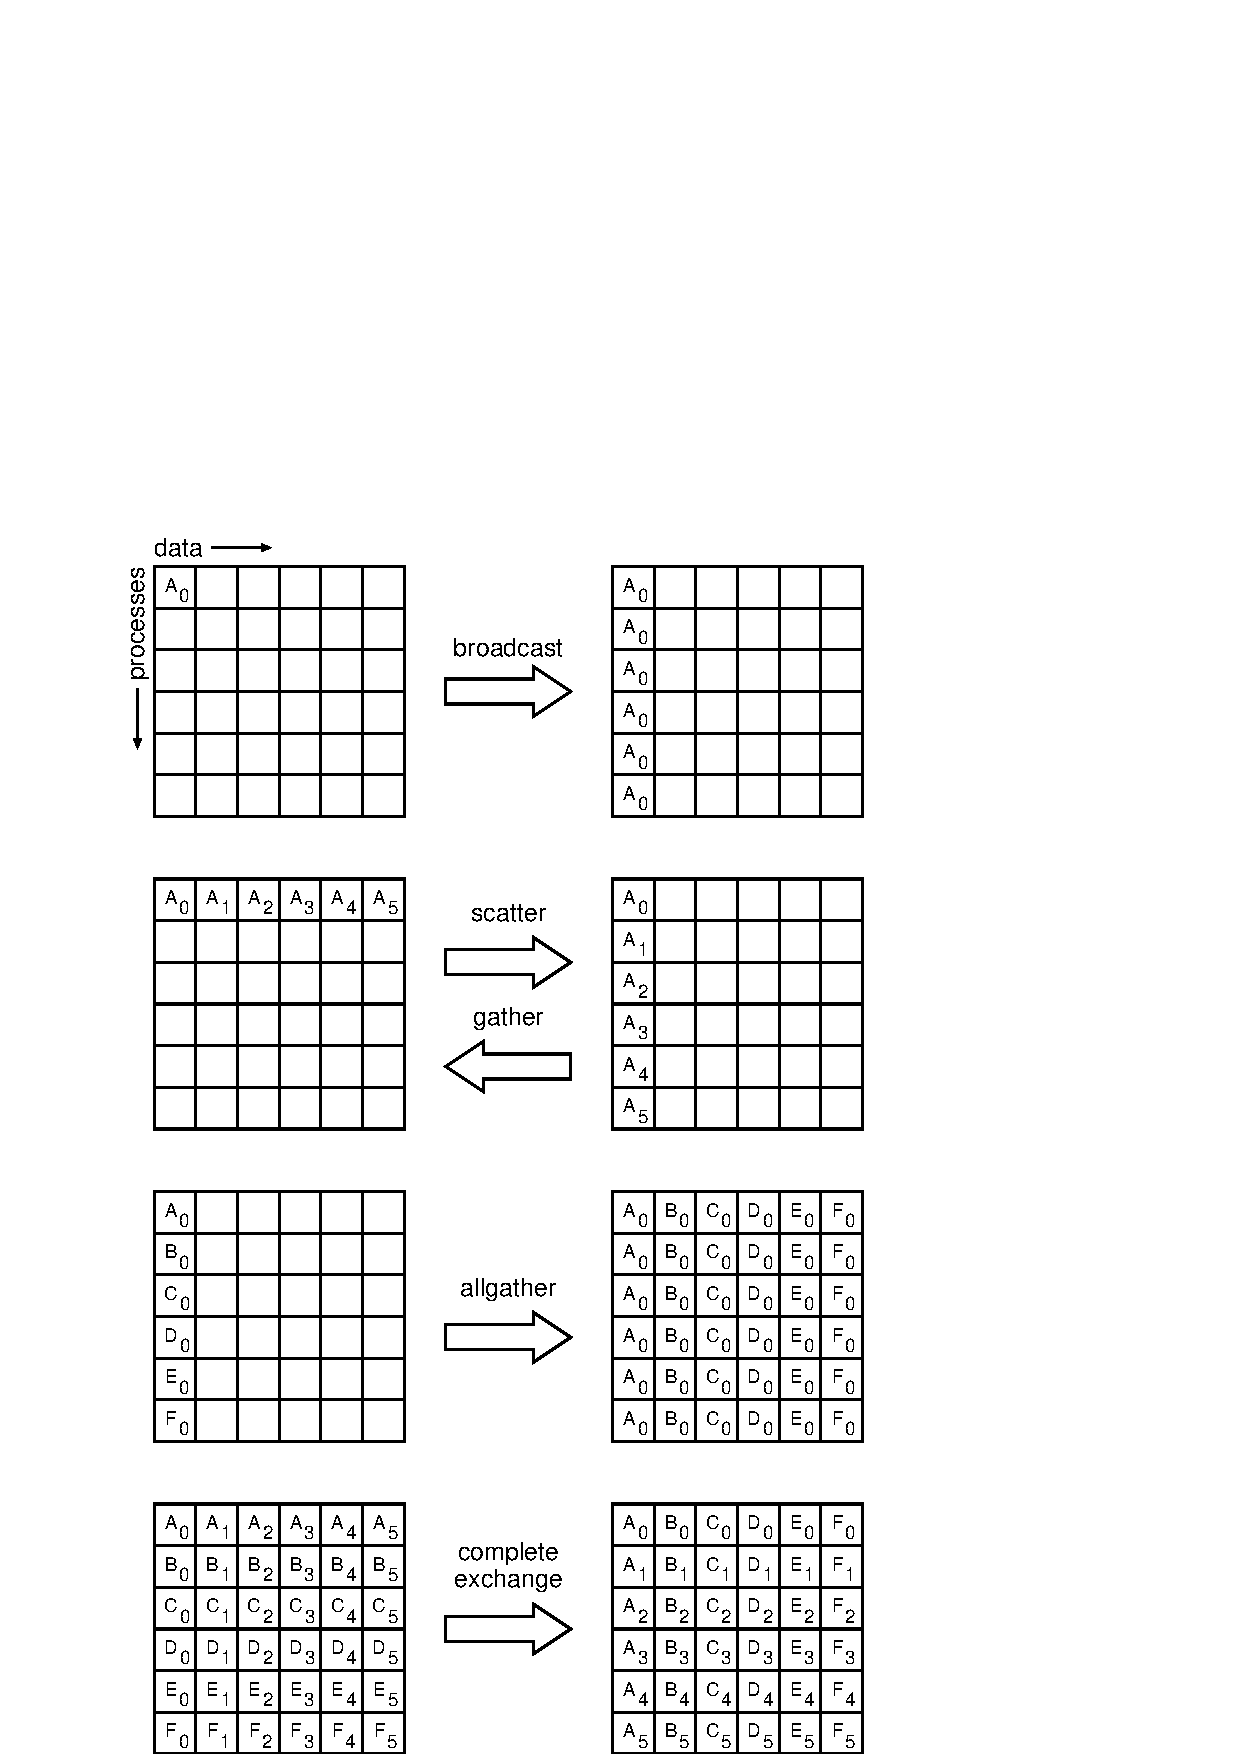
\includegraphics[scale=0.9]{figures/coll-fig1-22}}
  \caption[Collective communications, an overview]{Collective move functions illustrated
  for a group of six \MPI/ processes. In each case, each row of boxes
  represents data locations in one \MPI/ process. Thus, in the broadcast,
  initially just the first \MPI/ process contains the data $A_0$, but after the
  broadcast all \MPI/ processes contain it.}
  \label{fig:collcom}
\end{figure}

One of the key arguments
in a call to a collective routine
is a communicator that defines the group
or groups
of participating \MPI/ processes and provides a context for the operation.
This is discussed further in Section~\ref{sec:coll-communicator}.
The syntax and semantics of the collective operations are\mpitermindex{semantics!collective communications}
defined to be consistent with the syntax and semantics of the
point-to-point operations. Thus, general datatypes are allowed
and must match between sending and receiving \MPI/ processes as specified
in
Chapter~\ref{chap:datatypes}.
Several collective routines such as broadcast and gather have
a single originating or receiving \MPI/ process.
Such an \MPI/ process is
called the \mpitermdef{root}.
Some arguments in the collective functions are specified as
``significant only at root,'' and are ignored for all
participants except the root.

\begin{users}
Note that the programmer is still responsible for avoiding undefined behavior in the host language by not passing uninitialized values to \mpi/ procedure calls.
\end{users}

The reader is referred to Chapter~\ref{chap:datatypes}
for information concerning communication buffers,
general datatypes and type matching rules, and to
Chapter~\ref{chap:context} for information on how to define groups and
create communicators.

The type-matching conditions for the collective operations are more
strict than the corresponding conditions between sender and receiver
in point-to-point.  Namely, for collective operations,
the amount of data sent must exactly
match the amount of data specified by the receiver.
Different
type maps (the layout in memory, see Section~\ref{sec:pt2pt-datatype})
between sender and receiver are still allowed.

Collective operations can (but are not required to)
complete as soon as the
caller's
participation in the collective communication is
finished.  A blocking operation is
complete as soon as the call returns. A nonblocking (immediate) call
requires a separate completion call (cf.\ Section~\ref{sec:pt2pt-nonblock}).
The completion
of a collective operation indicates that the caller
is free to modify locations in the
communication buffer.  It does not indicate that other \MPI/ processes in
the group have completed or even
started the operation (unless otherwise
implied by
the description of the operation).
Thus, a collective communication operation may, or may not,
have the effect of synchronizing all participating \MPI/ processes.

Collective communication calls may use the same
communicators as point-to-point communication; \MPI/ guarantees that
messages generated on behalf of collective communication calls will not
be confused with messages generated by point-to-point communication.
The collective operations do not have a message tag argument.
A more detailed discussion of correct use of collective
routines is found in Section~\ref {coll:correct}.

\begin{rationale}
The equal-data restriction (on type matching) was made so
as to avoid the complexity
of providing a facility analogous to the status
argument of \mpifunc{MPI\_RECV} for discovering the amount of data sent.
Some of the collective routines would require an array of status values.

The statements about synchronization are made so as to allow a variety
of implementations of the collective functions.

\end{rationale}

\begin{users}
It is dangerous to rely on synchronization
side-effects of the collective operations for program correctness.
For example, even though a particular implementation may
provide a broadcast routine
with a side-effect of synchronization, the standard does not require
this, and a program that relies on this will not be portable.

On the other hand, a correct, portable program must allow for the fact
that a collective call \emph{may} be synchronizing.  Though one cannot
rely on any synchronization side-effect, one must program so as to allow
it.  These issues are discussed further in Section~\ref{coll:correct}.
\end{users}

\begin{implementors}
\sloppy %%ALLOWLATEX%%
While vendors may write optimized collective routines matched to
their architectures, a complete library of the collective communication
routines can be written entirely using the \MPI/ point-to-point communication
functions and a few auxiliary functions.  If implementing on top of
point-to-point, a hidden, special communicator\mpitermindex{communicator!hidden} might
be created for the
collective operation so as to avoid interference with any on-going
point-to-point communication at the time of the collective call.  This
is discussed further in Section~\ref{coll:correct}.
\end{implementors}

Many of the descriptions of the collective routines provide illustrations in
terms of blocking \MPI/ point-to-point routines.  These are intended solely to
indicate what data is sent or received by which \MPI/ process.  Many of these
examples
are \emph{not} correct \MPI/ programs; for purposes of simplicity, they often
assume infinite buffering.


\section{Communicator Argument}
\label{sec:coll-communicator}

The key concept of the collective functions is to have a
group or groups
of participating \MPI/ processes.
The routines do not have group identifiers as explicit arguments.
Instead, there is a communicator argument.
Groups and communicators are discussed in full detail in Chapter~\ref{chap:context}.
For the purposes of this chapter, it is sufficient to know that there
are two types of communicators:
\mpitermdefni{intra-communicators}\mpitermdefindex{intra-communicator} and
\mpitermdefni{inter-communicators}\mpitermdefindex{inter-communicator}.
An intra-communicator can be thought of as an identifier for a single group of \MPI/ processes
linked with a context.  An inter-communicator identifies two distinct groups of \MPI/ processes
linked with a context.


\subsection{Specifics for Intra-Communicator Collective Operations}
\mpitermtitleindex{intra-communicator!collective operations}
All \MPI/ processes in the group identified by the intra-communicator must call
the collective routine.

In many cases,
collective communication can occur ``in place''
for intra-communicators,
with the output
buffer being identical to the input buffer.  This is specified by
providing a special argument value, \mpiconstmain{MPI\_IN\_PLACE}, instead of the
send buffer or the receive buffer argument,
depending on the operation performed.

\begin{rationale}
The ``in place'' operations are provided to reduce unnecessary memory motion by
both the \MPI/ implementation and by the user.  Note that while the simple check
of testing whether the send and receive buffers have the same address will
work for some cases (e.g., \mpifunc{MPI\_ALLREDUCE}), they are inadequate in
others (e.g., \mpifunc{MPI\_GATHER}, with \mpiarg{root} not equal to zero).  Further,
Fortran explicitly prohibits aliasing of arguments; the approach of using a
special value to denote ``in place'' operation eliminates that difficulty.
\end{rationale}

\begin{users}
By allowing the ``in place'' option, the receive buffer in many of the
collective calls becomes a send-and-receive buffer.  For this reason, a
Fortran binding that includes \code{INTENT} must mark these as \code{INOUT},
not \code{OUT}.

Note that \mpiconstskip{MPI\_IN\_PLACE} is a special kind of value; it has the
same
restrictions on its use that \mpiconst{MPI\_BOTTOM} has
(not usable in Fortran for initialization or assignment).
See Section~\ref{subsec:named-constants}.
\end{users}

\subsection{Applying Collective Operations to Inter-Communicators}
\mpitermtitleindex{inter-communicator!collective operations}
\label{sec:collective-2}
\label{sec:MPI-coll}

To understand how collective operations apply to inter-communicators,
we can view most \MPI/ intra-communicator
collective operations as fitting one of the following categories (see, for
instance,
\cite{skjellum.doss.viswanathan.94}):
\begin{description}
\item[All-To-All] All \MPI/ processes contribute to the result.  All \MPI/ processes
  receive the result.
  \begin{itemize}
  \item \mpifunc{MPI\_ALLGATHER}, \mpifunc{MPI\_IALLGATHER}, \mpifunc{MPI\_ALLGATHER\_INIT},
  \mpifunc{MPI\_ALLGATHERV}, \mpifunc{MPI\_IALLGATHERV}, \mpifunc{MPI\_ALLGATHERV\_INIT}
  \item \mpifunc{MPI\_ALLTOALL}, \mpifunc{MPI\_IALLTOALL}, \mpifunc{MPI\_ALLTOALL\_INIT},
  \mpifunc{MPI\_ALLTOALLV}, \mpifunc{MPI\_IALLTOALLV}, \mpifunc{MPI\_ALLTOALLV\_INIT},
  \mpifunc{MPI\_ALLTOALLW}, \mpifunc{MPI\_IALLTOALLW}, \mpifunc{MPI\_ALLTOALLW\_INIT}
  \item \mpifunc{MPI\_ALLREDUCE}, \mpifunc{MPI\_IALLREDUCE}, \mpifunc{MPI\_ALLREDUCE\_INIT},
  \mpifunc{MPI\_REDUCE\_SCATTER\_BLOCK}, \mpifunc{MPI\_IREDUCE\_SCATTER\_BLOCK},
  \mpifunc{MPI\_REDUCE\_SCATTER\_BLOCK\_INIT},
  \mpifunc{MPI\_REDUCE\_SCATTER},   \mpifunc{MPI\_IREDUCE\_SCATTER},
  \mpifunc{MPI\_REDUCE\_SCATTER\_INIT}
  \item \mpifunc{MPI\_BARRIER}, \mpifunc{MPI\_IBARRIER}, \mpifunc{MPI\_BARRIER\_INIT}
  \end{itemize}
\item[All-To-One] All \MPI/ processes contribute to the result.  One \MPI/ process
  receives the result.
  \begin{itemize}
  \item \mpifunc{MPI\_GATHER}, \mpifunc{MPI\_IGATHER}, \mpifunc{MPI\_GATHER\_INIT},
  \mpifunc{MPI\_GATHERV}, \mpifunc{MPI\_IGATHERV}, \mpifunc{MPI\_GATHERV\_INIT}
  \item \mpifunc{MPI\_REDUCE}, \mpifunc{MPI\_IREDUCE}, \mpifunc{MPI\_REDUCE\_INIT},
  \end{itemize}
\item[One-To-All] One \MPI/ process contributes to the result.  All \MPI/ processes
  receive the result.
  \begin{itemize}
  \item \mpifunc{MPI\_BCAST}, \mpifunc{MPI\_IBCAST}, \mpifunc{MPI\_BCAST\_INIT}
  \item \mpifunc{MPI\_SCATTER}, \mpifunc{MPI\_ISCATTER}, \mpifunc{MPI\_SCATTER\_INIT},
  \mpifunc{MPI\_SCATTERV}, \mpifunc{MPI\_ISCATTERV}, \mpifunc{MPI\_SCATTERV\_INIT}
  \end{itemize}
\item[Other:] Collective operations that do not fit into one of the above
  categories.
  \begin{itemize}
  \item \mpifunc{MPI\_SCAN}, \mpifunc{MPI\_ISCAN}, \mpifunc{MPI\_SCAN\_INIT}
  \mpifunc{MPI\_EXSCAN}, \mpifunc{MPI\_IEXSCAN}, \mpifunc{MPI\_EXSCAN\_INIT}
  \end{itemize}
\end{description}

%%%%%%%%%%%%%%%%%%
%%%%%%%%%%%%%%%%%%

The application of collective communication to
inter-communicators is best described in terms of two groups.
For example, an all-to-all
\mpifunc{MPI\_ALLGATHER} operation can be described as collecting data
from all members of one group with the result appearing in all members
of the other group (see Figure~\ref{fig:collective-allgather}).  As another
example, a one-to-all \mpifunc{MPI\_BCAST} operation sends data from one
member of one group to all members of the other group.
Collective computation operations such as \mpifunc{MPI\_REDUCE\_SCATTER} have
a
similar interpretation (see Figure~\ref{fig:collective-reduce_scatter}).
For intra-communicators, these two groups
are the same.  For inter-communicators, these two groups are distinct.
For the all-to-all operations, each such operation is described in two phases,
so that it
has a symmetric, full-duplex behavior.

The following collective operations also apply to inter-communicators:
\begin{itemize}
\item \mpifunc{MPI\_BARRIER}, \mpifunc{MPI\_IBARRIER}, \mpifunc{MPI\_BARRIER\_INIT},
\item \mpifunc{MPI\_BCAST}, \mpifunc{MPI\_IBCAST}, \mpifunc{MPI\_BCAST\_INIT},
\item \mpifunc{MPI\_GATHER}, \mpifunc{MPI\_IGATHER}, \mpifunc{MPI\_GATHER\_INIT},
      \mpifunc{MPI\_GATHERV}, \mpifunc{MPI\_IGATHERV}, \mpifunc{MPI\_GATHERV\_INIT},
\item \mpifunc{MPI\_SCATTER}, \mpifunc{MPI\_ISCATTER}, \mpifunc{MPI\_SCATTER\_INIT},
      \mpifunc{MPI\_SCATTERV}, \mpifunc{MPI\_ISCATTERV}, \mpifunc{MPI\_SCATTERV\_INIT},
\item \mpifunc{MPI\_ALLGATHER}, \mpifunc{MPI\_IALLGATHER}, \mpifunc{MPI\_ALLGATHER\_INIT},
      \mpifunc{MPI\_ALLGATHERV}, \mpifunc{MPI\_IALLGATHERV}, \mpifunc{MPI\_ALLGATHERV\_INIT},
\item \mpifunc{MPI\_ALLTOALL}, \mpifunc{MPI\_IALLTOALL}, \mpifunc{MPI\_ALLTOALL\_INIT},
      \mpifunc{MPI\_ALLTOALLV}, \mpifunc{MPI\_IALLTOALLV}, \mpifunc{MPI\_ALLTOALLV\_INIT},
      \mpifunc{MPI\_ALLTOALLW}, \mpifunc{MPI\_IALLTOALLW}, \mpifunc{MPI\_ALLTOALLW\_INIT},
\item \mpifunc{MPI\_ALLREDUCE}, \mpifunc{MPI\_IALLREDUCE}, \mpifunc{MPI\_ALLREDUCE\_INIT},
      \mpifunc{MPI\_REDUCE}, \mpifunc{MPI\_IREDUCE}, \mpifunc{MPI\_REDUCE\_INIT},
\item \mpifunc{MPI\_REDUCE\_SCATTER\_BLOCK}, \mpifunc{MPI\_IREDUCE\_SCATTER\_BLOCK},
\mpifunc{MPI\_REDUCE\_SCATTER\_BLOCK\_INIT}, \mpifunc{MPI\_REDUCE\_SCATTER},
\mpifunc{MPI\_IREDUCE\_SCATTER}, \mpifunc{MPI\_REDUCE\_SCATTER\_INIT}.
\end{itemize}

\begin{figure}[htpb]
  \centerline{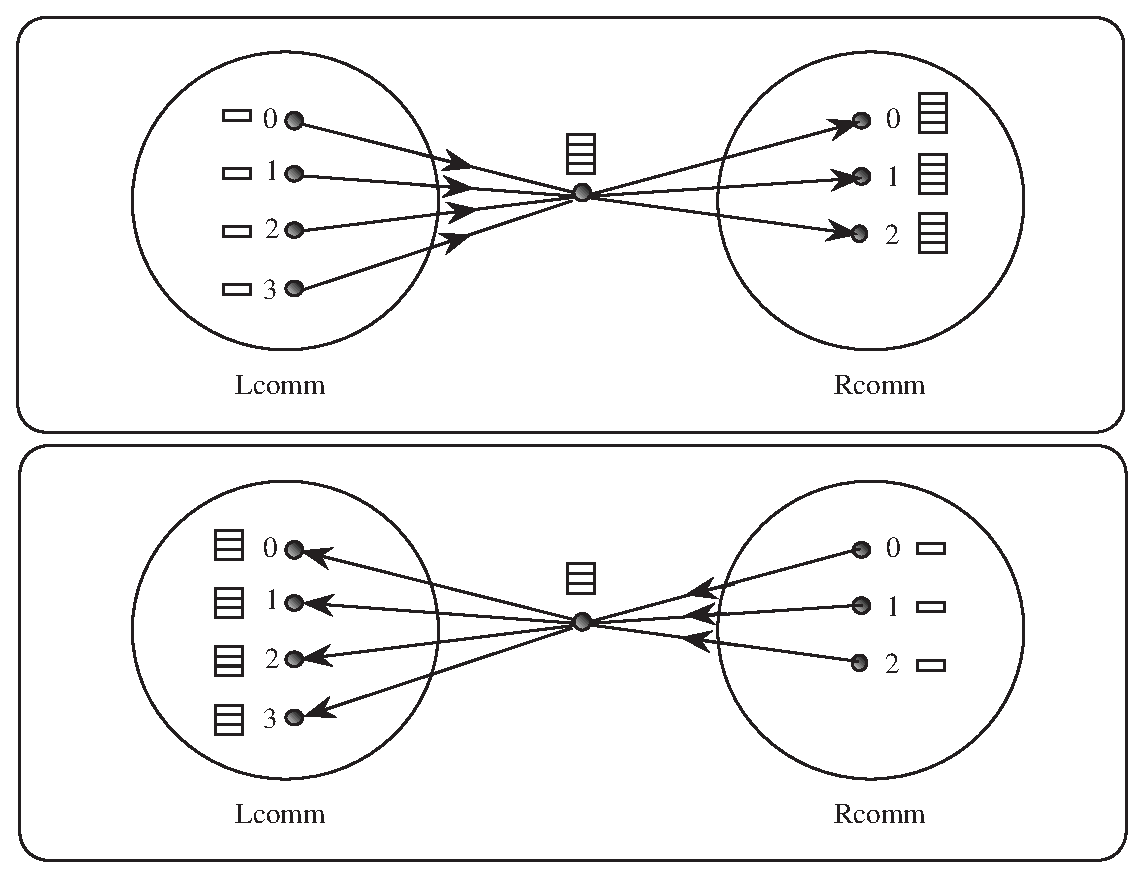
\includegraphics[width=4.0in]{figures/collective-allgather}}
  \caption[Inter-communicator allgather]{Inter-communicator allgather.  The focus of data to one \MPI/ process is
    represented, not mandated by the semantics.
    The two phases do allgathers in both directions.}
  \label{fig:collective-allgather}
\end{figure}

\begin{figure}[htpb]
  \centerline{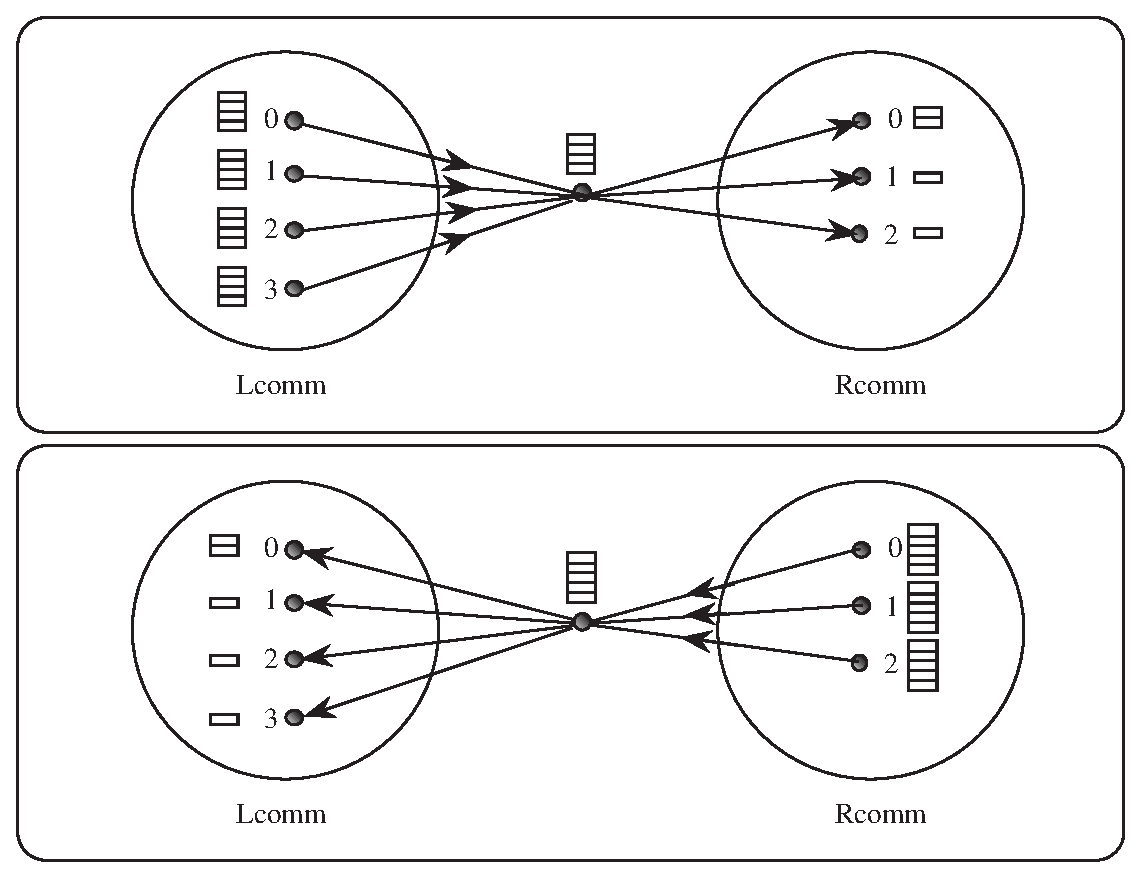
\includegraphics[width=4.0in]{figures/collective-reduce_scatter}}
  \caption[Inter-communicator reduce-scatter]{Inter-communicator reduce-scatter.  The focus of data to one \MPI/ process
    is represented, not mandated by the semantics.
    The two phases do reduce-scatters in both directions.}
  \label{fig:collective-reduce_scatter}
\end{figure}

\subsection{Specifics for Inter-Communicator Collective Operations}
\mpitermtitleindex{inter-communicator!collective operations}
All \MPI/ processes in both groups identified by the inter-communicator must call
the collective routine.

Note that the ``in place'' option for intra-communicators does not apply to
inter-communicators since in the inter-communicator case there is no
communication from an \MPI/ process to itself.

For inter-communicator collective communication, if
the
operation is in the All-To-One or One-To-All categories,
then the transfer is
unidirectional.
The direction of the transfer is indicated
by a special value of the \mpiarg{root} argument.
In this case, for the group containing the root, all \MPI/ processes in
the group must call the routine using a special argument for the root.
For this, the
root uses the special value \mpiconstmain{MPI\_ROOT}; all other
\MPI/ processes
in the same group as the root use \mpiconst{MPI\_PROC\_NULL}.
All \MPI/ processes in the other group (the group that
is the remote group relative to the root) must call the collective
routine and provide the rank of the root.
If the operation is in the All-To-All category,
then the transfer is bidirectional.

\begin{rationale}
Operations in the All-To-One
and One-To-All categories are unidirectional by nature, and there is a clear
way of specifying direction.
Operations in the All-To-All category will often occur as part of
an exchange, where it makes sense to communicate in both  directions at once.
\end{rationale}

\section{Barrier Synchronization}
\mpitermtitleindex{barrier synchronization}
\label{sec:coll-barrier}

\begin{mpi-binding}
    function_name("MPI_Barrier")
    parameter("comm", "COMMUNICATOR", desc=r"communicator")
\end{mpi-binding}

If \mpiarg{comm} is an intra-communicator,
\mpifunc{MPI\_BARRIER} blocks the caller until all group members have called
it. The call returns at any \MPI/ process only after all group members have
entered the call.

If \mpiarg{comm} is an inter-communicator, \mpifunc{MPI\_BARRIER} involves two groups.
The call returns at \MPI/ processes in one group (group A) of the inter-communicator
only after all members of the other group (group B) have entered the call (and vice
versa).  An \MPI/ process may return from the call before all \MPI/ processes in its own group
have entered the call.

\section{Broadcast}
\mpitermtitleindex{broadcast}
\label{sec:coll-broadcast}

\begin{mpi-binding}
    function_name("MPI_Bcast")
    parameter(
        "buffer", "BUFFER", desc=r"starting address of buffer", direction="inout"
    )
    parameter(
        "count", "POLYXFER_NUM_ELEM_NNI", desc=r"number of entries in buffer"
    )
    parameter("datatype", "DATATYPE", desc=r"datatype of buffer")
    parameter("root", "RANK", desc=r"rank of the root")
    parameter("comm", "COMMUNICATOR", desc=r"communicator")
\end{mpi-binding}

If \mpiarg{comm} is an intra-communicator,
\mpifunc{MPI\_BCAST} broadcasts a message from
the \MPI/ process with rank \mpiarg{root} to all \MPI/ processes
of the group, itself included.
It is called by all members of
the
group using the same arguments for
\mpiarg{comm}
and
\mpiarg{root}.
On return, the
content of the root's buffer is copied to all other \MPI/ processes.

General, derived datatypes are allowed for \mpiarg{datatype}.
The type signature of \mpiarg{count}, \mpiarg{datatype} on any \MPI/ process must
be equal to the type signature of \mpiarg{count}, \mpiarg{datatype} at the root.
This implies that the amount of data sent must be equal to the amount received,
pairwise between each \MPI/ process and the root.
\mpifunc{MPI\_BCAST} and all other data-movement collective routines
make this restriction.
Distinct type maps between sender and receiver are still allowed.

The ``in place'' option is not meaningful here.

If \mpiarg{comm} is an inter-communicator, then the call involves all
\MPI/ processes in the inter-communicator, but with one group (group A) defining the
root.  All \MPI/ processes in the other group (group B) pass the same value
in argument
\mpiarg{root}, which is the rank of the root in group A.  The root
passes the value \mpiconstskip{MPI\_ROOT} in \mpiarg{root}.
All other \MPI/ processes in group A pass the value \mpiconst{MPI\_PROC\_NULL} in
\mpiarg{root}.
Data is broadcast from the root to all \MPI/ processes in group B.
The
buffer arguments of the \MPI/ processes in group B must be consistent with
the buffer argument of the root.

\subsection{Example using \texorpdfstring{\mpifunc{MPI\_BCAST}}{MPI\_BCAST}}

The examples in this section use intra-communicators.

\begin{example}
\label{coll-exZ}
\Exindex{C}{Broadcast}{MPI\_Bcast}%
Broadcast 100 \code{int}s from \MPI/ process \code{0} to every \MPI/ process in the group.

%%HEADER
%%LANG: C
%%FRAGMENT
%%SKIPELIPSIS
%%ENDHEADER
\begin{lstlisting}[language={[MPI]C}]
MPI_Comm comm;
int array[100];
int root=0;
...
MPI_Bcast(array, 100, MPI_INT, root, comm);
\end{lstlisting}
As in many of our example code fragments, we assume that some
of the variables (such as \code{comm} in the above) have been assigned
appropriate values.
\end{example}

\section{Gather}
\mpitermtitleindex{gather}
\label{sec:coll-gather}

\begin{mpi-binding}
    function_name("MPI_Gather")
    parameter(
        "sendbuf",
        "BUFFER",
        desc=r"starting address of send buffer",
        constant=True,
    )
    parameter(
        "sendcount",
        "POLYXFER_NUM_ELEM_NNI",
        desc=r"number of elements in send buffer",
    )
    parameter("sendtype", "DATATYPE", desc=r"datatype of send buffer elements")
    parameter(
        "recvbuf",
        "BUFFER",
        desc=r"address of receive buffer",
        direction="out",
        root_only=True,
    )
    parameter(
        "recvcount",
        "POLYXFER_NUM_ELEM_NNI",
        desc=r"number of elements for any single receive",
        root_only=True,
    )
    parameter(
        "recvtype",
        "DATATYPE",
        desc=r"datatype of recv buffer elements",
        root_only=True,
    )
    parameter("root", "RANK", desc=r"rank of receiving \MPI/ process")
    parameter("comm", "COMMUNICATOR", desc=r"communicator")
\end{mpi-binding}

%%FIXME: This description mixes C and language-independent forms of the MPI
%% routines.  The behavior of MPI should be defined in language-independent
%% terms.
If \mpiarg{comm} is an intra-communicator,
each \MPI/ process (the root included) sends the contents of its send
buffer to the root.  The root receives the messages and
stores them in rank order.
The outcome is \emph{as if} each of the \mpicode{n} \MPI/ processes in the group
(including the root) had executed a call to
\begin{mpicodeblock}
MPI\_Send(sendbuf, sendcount, sendtype, root , ...),
\end{mpicodeblock}
\noindent and the
root had executed \mpicode{n} calls to
\begin{mpicodeblock}
MPI\_Recv(recvbuf+i$\cdot$ recvcount$\cdot$ extent(recvtype), recvcount, recvtype, i,...),
\end{mpicodeblock}
\noindent where \mpicode{extent(recvtype)} is the type extent obtained from a call to
\mpicode{MPI\_Type\_get\_extent}.

An alternative description is that the \mpicode{n} messages sent by the
processes in the group are concatenated in rank order, and the
resulting message is received by the root as if by a call to
\mpifunc{MPI\_RECV}\mpicode{(recvbuf, recvcount$\cdot$n, recvtype, ...)}.

The receive buffer is ignored for all nonroot \MPI/ processes.

General, derived datatypes are allowed for both \mpiarg{sendtype}
and \mpiarg{recvtype}.
The type signature of \mpiarg{sendcount}, \mpiarg{sendtype} on
each \MPI/ process
must be equal to the type signature of
\mpiarg{recvcount}, \mpiarg{recvtype} at the root.
This implies that the amount of data sent must be equal to the
amount of data received, pairwise between each \MPI/ process and the root.
Distinct type maps between sender and receiver \MPI/ processes are still allowed.

All arguments to the function are significant on the root,
while on other \MPI/ processes, only the arguments \mpiarg{sendbuf}, \mpiarg{sendcount},
\mpiarg{sendtype}, \mpiarg{root},
and
\mpiarg{comm} are significant.
The arguments \mpiarg{root} and \mpiarg{comm}
must have identical values on all \MPI/ processes.

The specification of counts and types
should not cause any location on the root to be written more than
once.  Such a call is erroneous.


Note that the \mpiarg{recvcount} argument at the root indicates
the number of items it receives from \emph{each} \MPI/ process, not the total number
of items it receives.

The ``in place'' option  for intra-communicators is specified by passing
\mpiconstskip{MPI\_IN\_PLACE} as
the value of \mpiarg{sendbuf} at the root.  In such a case,
\mpiarg{sendcount} and \mpiarg{sendtype} are ignored, and the
contribution of the root to the gathered vector is assumed to be already
in the correct place in the receive buffer.

If \mpiarg{comm} is an inter-communicator, then the call involves all
\MPI/ processes in the inter-communicator, but with one group (group A) defining the
root.  All \MPI/ processes in the other group (group B) pass the same value
in argument
\mpiarg{root}, which is the rank of the root in group A.  The root
passes the value \mpiconstskip{MPI\_ROOT} in \mpiarg{root}.
All other \MPI/ processes in group A pass the value \mpiconst{MPI\_PROC\_NULL} in
\mpiarg{root}.
Data is gathered from all \MPI/ processes in group B to the root.
The send
buffer arguments of the \MPI/ processes in group B must be consistent with
the receive buffer argument of the root.

\begin{mpi-binding}
    function_name("MPI_Gatherv")
    parameter(
        "sendbuf",
        "BUFFER",
        desc=r"starting address of send buffer",
        constant=True,
    )
    parameter(
        "sendcount",
        "POLYXFER_NUM_ELEM_NNI",
        desc=r"number of elements in send buffer",
    )
    parameter("sendtype", "DATATYPE", desc=r"datatype of send buffer elements")
    parameter(
        "recvbuf",
        "BUFFER",
        desc=r"address of receive buffer",
        direction="out",
        root_only=True,
    )
    parameter(
        "recvcounts",
        "POLYXFER_NUM_ELEM_NNI",
        desc=(
            r"nonnegative integer array (of length group size) containing "
            r"the number of elements that are received from each \MPI/ process"
        ),
        constant=True,
        length="*",
        root_only=True,
        suppress="lis_paren",
    )
    parameter(
        "displs",
        "POLYDISPLACEMENT",
        desc=(
            r"integer array (of length group size). Entry \mpicode{i} "
            r"specifies the displacement relative to \mpiarg{recvbuf} at "
            r"which to place the incoming data from \MPI/ process \mpicode{i}"
        ),
        constant=True,
        length="*",
        root_only=True,
        suppress="lis_paren",
    )
    parameter(
        "recvtype",
        "DATATYPE",
        desc=r"datatype of recv buffer elements",
        root_only=True,
    )
    parameter("root", "RANK", desc=r"rank of receiving \MPI/ process")
    parameter("comm", "COMMUNICATOR", desc=r"communicator")
\end{mpi-binding}

\mpifunc{MPI\_GATHERV} extends the functionality of \mpifunc{MPI\_GATHER}
by allowing a varying count of data from each \MPI/ process, since
\mpiarg{recvcounts}
is now an array.  It also allows more flexibility as to where the data
is placed on the root, by providing the new argument, \mpiarg{displs}.

If \mpiarg{comm} is an intra-communicator,
the outcome is \emph{as if} each \MPI/ process, including the root,
sends a message to the root,
\begin{mpicodeblock}
MPI\_Send(sendbuf, sendcount, sendtype, root, ...),
\end{mpicodeblock}
\noindent and the root executes \mpicode{n} receives,
\begin{mpicodeblock}
MPI\_Recv(recvbuf+displs[j]$\cdot$ extent(recvtype), recvcounts[j],
recvtype, i, ...).
\end{mpicodeblock}

The
data received from \MPI/ process \mpicode{j} is placed into \mpiarg{recvbuf} of the root
beginning at offset \mpiarg{displs[j]} elements (in terms of the
\mpiarg{recvtype}).

The receive buffer is ignored for all nonroot \MPI/ processes.

The type signature implied by \mpiarg{sendcount}, \mpiarg{sendtype} on \MPI/ process \mpicode{i}
must be equal to the type signature implied by \mpiarg{recvcounts[i]}, \mpiarg{recvtype}
at the root.
This implies that the amount of data sent must be equal to the
amount of data received, pairwise between each \MPI/ process and the root.
Distinct type maps between sender and receiver are still allowed,
as illustrated in Example~\ref{coll-exD}.

All arguments to the function are significant on the root,
while on other \MPI/ processes, only arguments \mpiarg{sendbuf}, \mpiarg{sendcount},
\mpiarg{sendtype}, \mpiarg{root},
and
\mpiarg{comm} are significant.
The arguments \mpiarg{root} and \mpiarg{comm}
must have identical values on all \MPI/ processes.

The specification of counts, types, and displacements
should not cause any location on the root to be written more than
once.  Such a call is erroneous.

% This is the same text as for Gather.
The ``in place'' option  for intra-communicators is specified by passing
\mpiconstskip{MPI\_IN\_PLACE} as
the value of \mpiarg{sendbuf} at the root.  In such a case,
\mpiarg{sendcount} and \mpiarg{sendtype} are ignored, and the
contribution of the root to the gathered vector is assumed to be already
in the correct place in the receive buffer.

If \mpiarg{comm} is an inter-communicator, then the call involves all
\MPI/ processes in the inter-communicator, but with one group (group A) defining the
root.  All \MPI/ processes in the other group (group B) pass the same value
in argument
\mpiarg{root}, which is the rank of the root in group A.  The root
passes the value \mpiconstskip{MPI\_ROOT} in \mpiarg{root}.
All other \MPI/ processes in group A pass the value \mpiconst{MPI\_PROC\_NULL} in
\mpiarg{root}.
Data is gathered from all \MPI/ processes in group B to the root.
The send
buffer arguments of the \MPI/ processes in group B must be consistent with
the receive buffer argument of the root.

\subsection{Examples using \texorpdfstring{\mpifunc{MPI\_GATHER}}{MPI\_GATHER} and \texorpdfstring{\mpifunc{MPI\_GATHERV}}{MPI\_GATHERV}}

The examples in this section use intra-communicators.

\begin{example}
\label{coll-exA}
\Exindex{C}{Gather}{MPI\_Gather}%
Gather 100 \code{int}s from every \MPI/ process in group to the root. See
Figure~\ref{fig-coll-exA}.

%%HEADER
%%LANG: C
%%FRAGMENT
%%SKIPELIPSIS
%%ENDHEADER
\begin{lstlisting}[language={[MPI]C}]
MPI_Comm comm;
int gsize,sendarray[100];
int root, *rbuf;
...
MPI_Comm_size(comm, &gsize);
rbuf = (int *)malloc(gsize*100*sizeof(int));
MPI_Gather(sendarray, 100, MPI_INT, rbuf, 100, MPI_INT, root, comm);
\end{lstlisting}
\end{example}



\begin{example}
\label{coll-exAa}
\Exindex{C}{Gather with allocation at the root}{MPI\_Gather}%
Previous example modified---only the root allocates memory for the
receive buffer. The argument \mpiarg{rbuf} still must be initialized on all processes.


%%HEADER
%%LANG: C
%%FRAGMENT
%%SKIPELIPSIS
%%ENDHEADER
\begin{lstlisting}[language={[MPI]C}]
MPI_Comm comm;
int gsize,sendarray[100];
int root, myrank, *rbuf = NULL;
...
MPI_Comm_rank(comm, &myrank);
if (myrank == root) {
   MPI_Comm_size(comm, &gsize);
   rbuf = (int *)malloc(gsize*100*sizeof(int));
}
MPI_Gather(sendarray, 100, MPI_INT, rbuf, 100, MPI_INT, root, comm);
\end{lstlisting}
\end{example}


\begin{figure}
  \centerline{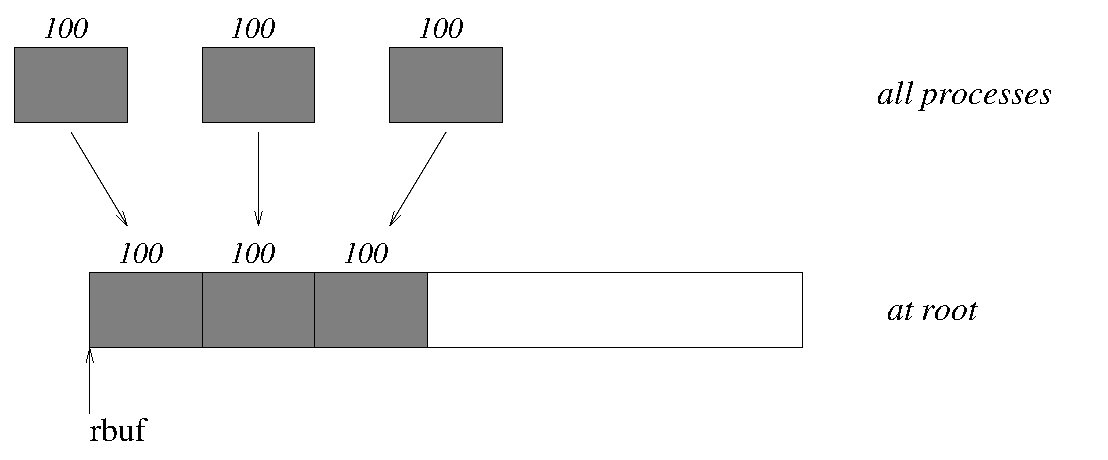
\includegraphics[width=3.50in]{figures/mycoll-fig2}}
  \caption[Gather example]{The root gathers 100 \code{int}s from
    each \MPI/ process in the group}
  \label{fig-coll-exA}
\end{figure}

\begin{example}
\label{coll-exB}
\Exindex{C}{Gather with datatype}{MPI\_Type\_contiguous,MPI\_Type\_commit,MPI\_Gather}%
Do the same as the previous example, but use a derived datatype.  Note that
the type cannot be the entire set of \code{gsize*100 int}s since type matching
is defined pairwise between the root and each \MPI/ process in the gather.

%%HEADER
%%LANG: C
%%FRAGMENT
%%SKIPELIPSIS
%%ENDHEADER
\begin{lstlisting}[language={[MPI]C}]
MPI_Comm comm;
int gsize,sendarray[100];
int root, *rbuf;
MPI_Datatype rtype;
...
MPI_Comm_size(comm, &gsize);
MPI_Type_contiguous(100, MPI_INT, &rtype);
MPI_Type_commit(&rtype);
rbuf = (int *)malloc(gsize*100*sizeof(int));
MPI_Gather(sendarray, 100, MPI_INT, rbuf, 1, rtype, root, comm);
\end{lstlisting}
\end{example}

\begin{example}
\label{coll-exC}
\Exindex{C}{Gatherv}{MPI\_Gatherv}%
Now have each \MPI/ process send 100 \code{int}s to the root, but place each set (of 100)
\code{stride int}s apart at the receiving end. Use \mpifunc{MPI\_GATHERV}
and the \mpiarg{displs}
argument to achieve this effect. Assume \code{stride} $\geq 100$.
See Figure~\ref{fig-coll-exC}.

%%HEADER
%%LANG: C
%%FRAGMENT
%%SKIPELIPSIS
%%ENDHEADER
\begin{lstlisting}[language={[MPI]C}]
MPI_Comm comm;
int gsize,sendarray[100];
int root, *rbuf, stride;
int *displs,i,*rcounts;

...

MPI_Comm_size(comm, &gsize);
rbuf = (int *)malloc(gsize*stride*sizeof(int));
displs = (int *)malloc(gsize*sizeof(int));
rcounts = (int *)malloc(gsize*sizeof(int));
for (i=0; i<gsize; ++i) {
    displs[i] = i*stride;
    rcounts[i] = 100;
}
MPI_Gatherv(sendarray, 100, MPI_INT, rbuf, rcounts, displs, MPI_INT,
            root, comm);
\end{lstlisting}

Note that the program is erroneous if \code{stride} $< 100$.
\end{example}

\begin{figure}
  \centerline{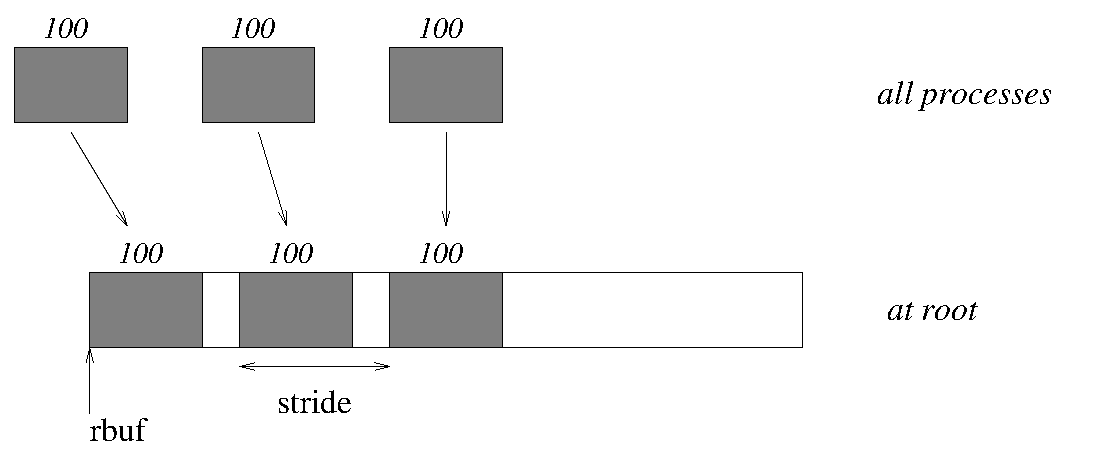
\includegraphics[width=3.50in]{figures/mycoll-fig3}}
  \caption[Gatherv example with strides]{The root gathers 100
    \code{int}s from each \MPI/ process
  in the group, each set is placed \code{stride int}s apart}
  \label{fig-coll-exC}
\end{figure}

\begin{example}
\label{coll-exD}
\Exindex{C}{Gatherv with datatype}{MPI\_Gatherv,MPI\_Type\_vector,MPI\_Type\_commit}%
Same as Example~\ref{coll-exC} on the receiving side, but send the
100 \code{int}s from the 0th column of a
100$\times$150 \code{int} array, in C.  See Figure~\ref{fig-coll-exD}.

%%HEADER
%%LANG: C
%%FRAGMENT
%%SKIPELIPSIS
%%ENDHEADER
\begin{lstlisting}[language={[MPI]C}]
MPI_Comm comm;
int gsize,sendarray[100][150];
int root, *rbuf, stride;
MPI_Datatype stype;
int *displs,i,*rcounts;

...

MPI_Comm_size(comm, &gsize);
rbuf = (int *)malloc(gsize*stride*sizeof(int));
displs = (int *)malloc(gsize*sizeof(int));
rcounts = (int *)malloc(gsize*sizeof(int));
for (i=0; i<gsize; ++i) {
    displs[i] = i*stride;
    rcounts[i] = 100;
}
/* Create datatype for 1 column of array
 */
MPI_Type_vector(100, 1, 150, MPI_INT, &stype);
MPI_Type_commit(&stype);
MPI_Gatherv(sendarray, 1, stype, rbuf, rcounts, displs, MPI_INT,
            root, comm);
\end{lstlisting}
\end{example}

\begin{figure}
  \centerline{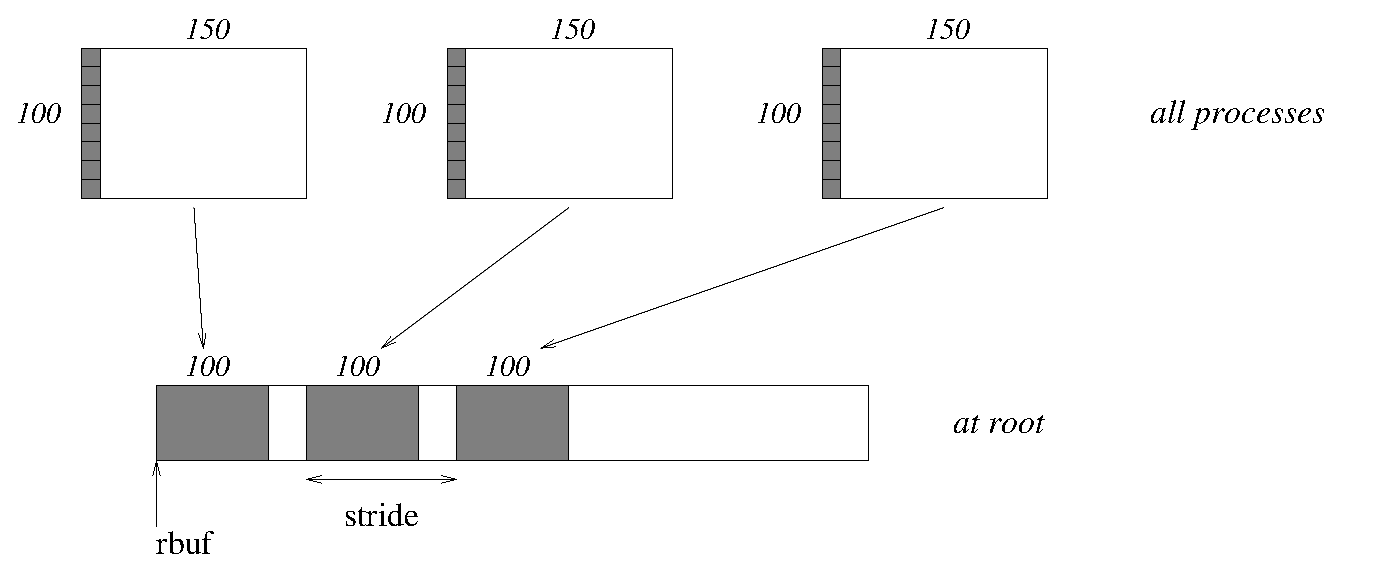
\includegraphics[width=4.00in]{figures/mycoll-fig4}}
  \caption[Gatherv example, 2-dimensional]{The root gathers column
    \code{0} of a 100$\times$150
  C array, and each set is placed \code{stride int}s apart}
  \label{fig-coll-exD}
\end{figure}

\begin{example}
\label{coll-exE}
\Exindex{C}{Gatherv with datatype}{MPI\_Gatherv,MPI\_Type\_vector,MPI\_Type\_commit}%
\MPI/ process \code{i} sends \code{(100-i) int}s from the \code{i}-th column of a
100 $\times$ 150 \code{int} array, in C.  It is received into a buffer with stride,
as in the previous two examples. See Figure~\ref{fig-coll-exE}.

%%HEADER
%%LANG: C
%%FRAGMENT
%%SKIPELIPSIS
%%ENDHEADER
\begin{lstlisting}[language={[MPI]C}]
MPI_Comm comm;
int gsize,sendarray[100][150],*sptr;
int root, *rbuf, stride, myrank;
MPI_Datatype stype;
int *displs,i,*rcounts;

...

MPI_Comm_size(comm, &gsize);
MPI_Comm_rank(comm, &myrank);
rbuf = (int *)malloc(gsize*stride*sizeof(int));
displs = (int *)malloc(gsize*sizeof(int));
rcounts = (int *)malloc(gsize*sizeof(int));
for (i=0; i<gsize; ++i) {
    displs[i] = i*stride;
    rcounts[i] = 100-i;     /* note change from previous example */
}
/* Create datatype for the column we are sending
 */
MPI_Type_vector(100-myrank, 1, 150, MPI_INT, &stype);
MPI_Type_commit(&stype);
/* sptr is the address of start of "myrank" column
 */
sptr = &sendarray[0][myrank];
MPI_Gatherv(sptr, 1, stype, rbuf, rcounts, displs, MPI_INT,
            root, comm);
\end{lstlisting}

Note that a different amount of data is received from each \MPI/ process.
\end{example}

\begin{figure}
  \centerline{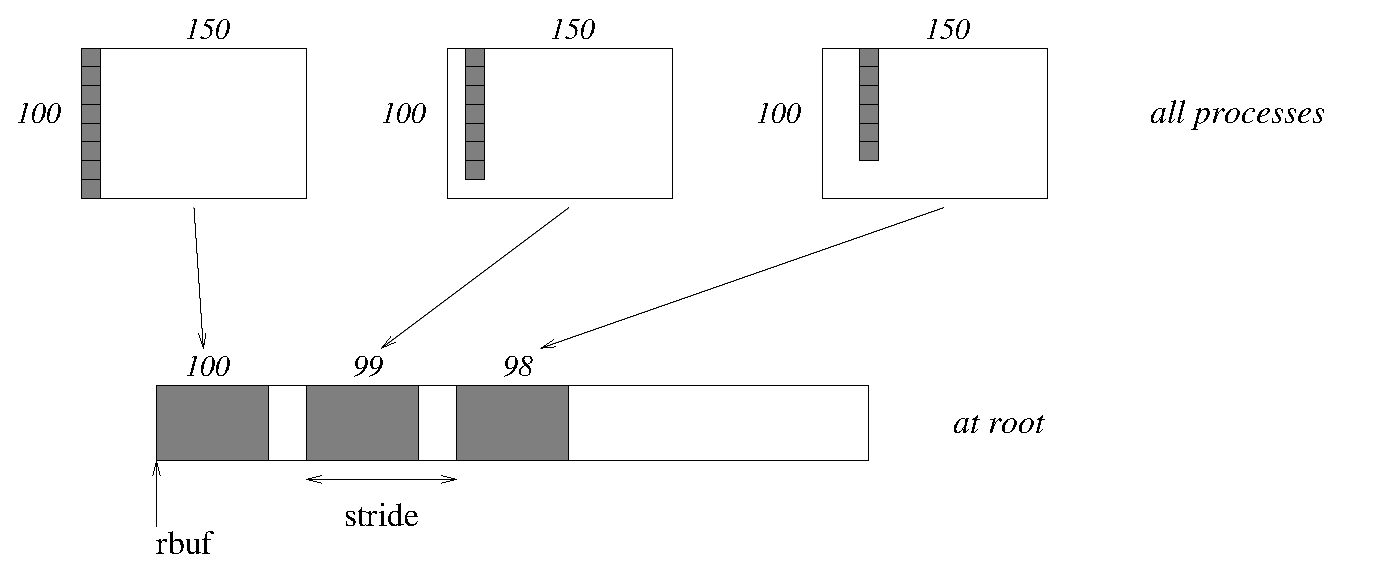
\includegraphics[width=4.00in]{figures/mycoll-fig5}}
  \caption[Gatherv example, 2-dimensional, subarrays with different sizes]{The
    root gathers \code{100-i int}s from
  column \code{i} of a 100$\times$150
  C array, and each set is placed \code{stride int}s apart}
  \label{fig-coll-exE}
\end{figure}

\begin{example}
\label{coll-exF}
\Exindex{C}{Gatherv with struct datatype}{MPI\_Gatherv,MPI\_Type\_create\_struct,MPI\_Type\_commit}%
Same as Example~\ref{coll-exE}, but done in a different way at the sending end.
We create a datatype that causes the correct striding at the
sending end so
that
we read a column of a C array.
A similar thing was done in Example~\ref{pt2pt-exFF},
Section~\ref{subsec:pt2pt-examples}.

%%HEADER
%%LANG: C
%%FRAGMENT
%%SKIPELIPSIS
%%ENDHEADER
\begin{lstlisting}[language={[MPI]C}]
MPI_Comm comm;
int gsize, sendarray[100][150], *sptr;
int root, *rbuf, stride, myrank;
MPI_Datatype stype;
int *displs, i, *rcounts;

...

MPI_Comm_size(comm, &gsize);
MPI_Comm_rank(comm, &myrank);
rbuf = (int *)malloc(gsize*stride*sizeof(int));
displs = (int *)malloc(gsize*sizeof(int));
rcounts = (int *)malloc(gsize*sizeof(int));
for (i=0; i<gsize; ++i) {
    displs[i] = i*stride;
    rcounts[i] = 100-i;
}
/* Create datatype for one int, with extent of entire row
 */
MPI_Type_create_resized(MPI_INT, 0, 150*sizeof(int), &stype);
MPI_Type_commit(&stype);
sptr = &sendarray[0][myrank];
MPI_Gatherv(sptr, 100-myrank, stype, rbuf, rcounts, displs, MPI_INT,
            root, comm);
\end{lstlisting}
\end{example}

\begin{example}
\label{coll-exG}
\Exindex{C}{Gatherv with vector datatype}{MPI\_Gatherv,MPI\_Type\_vector,MPI\_Type\_commit}%
Same as Example~\ref{coll-exE} at sending side, but
at receiving side we make the
stride between received blocks vary from block to block.
See Figure~\ref{fig-coll-exG}.

%%HEADER
%%LANG: C
%%FRAGMENT
%%SKIPELIPSIS
%%ENDHEADER
\begin{lstlisting}[language={[MPI]C}]
MPI_Comm comm;
int gsize,sendarray[100][150],*sptr;
int root, *rbuf, *stride, myrank, bufsize;
MPI_Datatype stype;
int *displs,i,*rcounts,offset;

...

MPI_Comm_size(comm, &gsize);
MPI_Comm_rank(comm, &myrank);

stride = (int *)malloc(gsize*sizeof(int));
...
/* stride[i] for i = 0 to gsize-1 is set somehow
 */

/* set up displs and rcounts vectors first
 */
displs = (int *)malloc(gsize*sizeof(int));
rcounts = (int *)malloc(gsize*sizeof(int));
offset = 0;
for (i=0; i<gsize; ++i) {
    displs[i] = offset;
    offset += stride[i];
    rcounts[i] = 100-i;
}
/* the required buffer size for rbuf is now easily obtained
 */
bufsize = displs[gsize-1]+rcounts[gsize-1];
rbuf = (int *)malloc(bufsize*sizeof(int));
/* Create datatype for the column we are sending
 */
MPI_Type_vector(100-myrank, 1, 150, MPI_INT, &stype);
MPI_Type_commit(&stype);
sptr = &sendarray[0][myrank];
MPI_Gatherv(sptr, 1, stype, rbuf, rcounts, displs, MPI_INT,
            root, comm);
\end{lstlisting}
\end{example}

\begin{figure}
  \centerline{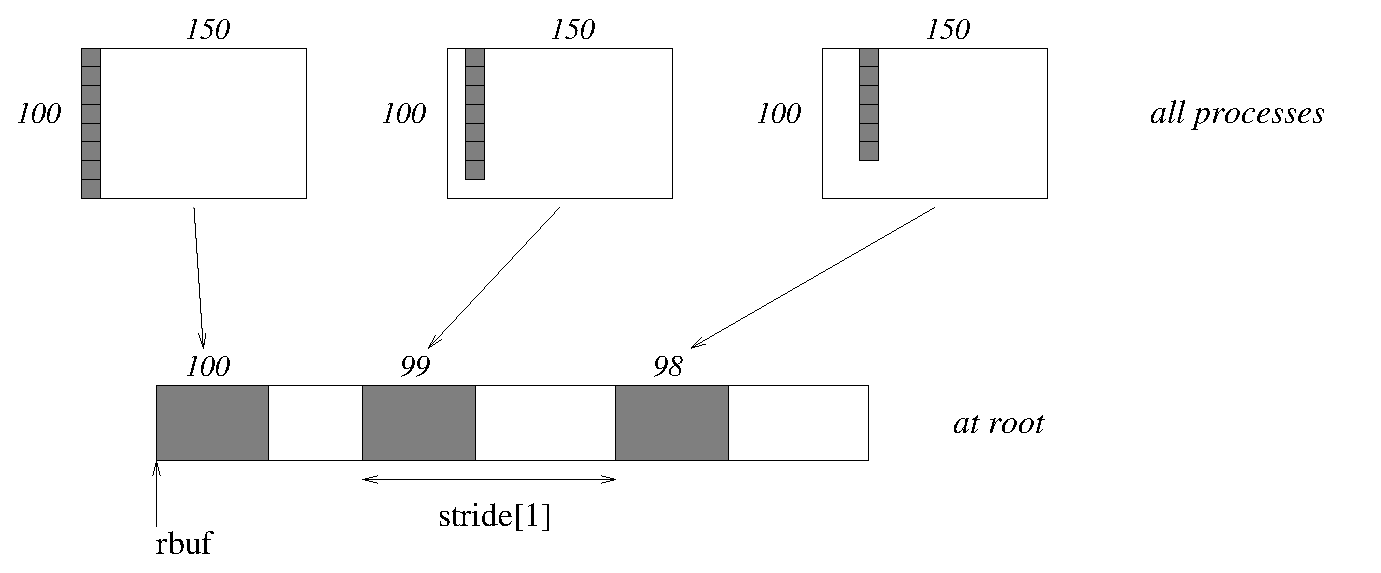
\includegraphics[width=4.00in]{figures/mycoll-fig6}}
  \caption[Gatherv example, 2-dimensional, subarrays with different sizes and
    strides]{The root gathers \code{100-i int}s from
  column \code{i} of a 100$\times$150
  C array, and each set is placed \code{stride[i] int}s apart (a varying
  stride)}
  \label{fig-coll-exG}
\end{figure}


\begin{example}
\label{coll-exH}
\Exindex{C}{Gather and Gatherv}{MPI\_Gather,MPI\_Gatherv,MPI\_Type\_create\_struct,MPI\_Type\_commit}%
\MPI/ process \code{i} sends \code{num int}s from the \code{i}-th column of a
100 $\times$ 150 \code{int} array, in C.  The complicating factor is that
the various values of \code{num} are not known to \code{root}, so a
separate gather must first be run to find these out.  The data is
placed contiguously at the receiving end.

%%HEADER
%%LANG: C
%%FRAGMENT
%%SKIPELIPSIS
%%ENDHEADER
\begin{lstlisting}[language={[MPI]C}]
MPI_Comm comm;
int gsize,sendarray[100][150],*sptr;
int root, *rbuf, myrank;
MPI_Datatype stype;
int *displs,i,*rcounts,num;

...

MPI_Comm_size(comm, &gsize);
MPI_Comm_rank(comm, &myrank);

/* First, gather nums to root
 */
rcounts = (int *)malloc(gsize*sizeof(int));
MPI_Gather(&num, 1, MPI_INT, rcounts, 1, MPI_INT, root, comm);
/* root now has correct rcounts, using these we set displs[] so that
 * data is placed contiguously (or concatenated) at the receiving end
 */
displs = (int *)malloc(gsize*sizeof(int));
displs[0] = 0;
for (i=1; i<gsize; ++i) {
    displs[i] = displs[i-1]+rcounts[i-1];
}
/* And, create receive buffer
 */
rbuf = (int *)malloc(gsize*(displs[gsize-1]+rcounts[gsize-1])
                                                      *sizeof(int));
/* Create datatype for one int, with extent of entire row
 */
MPI_Type_create_resized(MPI_INT, 0, 150*sizeof(int), &stype);
MPI_Type_commit(&stype);
sptr = &sendarray[0][myrank];
MPI_Gatherv(sptr, num, stype, rbuf, rcounts, displs, MPI_INT,
            root, comm);
\end{lstlisting}
\end{example}

\section{Scatter}
\mpitermtitleindex{scatter}
\label{sec:coll-scatter}

\begin{mpi-binding}
    function_name("MPI_Scatter")
    parameter(
        "sendbuf",
        "BUFFER",
        desc=r"address of send buffer",
        constant=True,
        root_only=True,
    )
    parameter(
        "sendcount",
        "POLYXFER_NUM_ELEM_NNI",
        desc=r"number of elements sent to each \MPI/ process",
        root_only=True,
    )
    parameter(
        "sendtype",
        "DATATYPE",
        desc=r"datatype of send buffer elements",
        root_only=True,
    )
    parameter(
        "recvbuf", "BUFFER", desc=r"address of receive buffer", direction="out"
    )
    parameter(
        "recvcount",
        "POLYXFER_NUM_ELEM_NNI",
        desc=r"number of elements in receive buffer",
    )
    parameter(
        "recvtype", "DATATYPE", desc=r"datatype of receive buffer elements"
    )
    parameter("root", "RANK", desc=r"rank of sending \MPI/ process")
    parameter("comm", "COMMUNICATOR", desc=r"communicator")
\end{mpi-binding}

\mpifunc{MPI\_SCATTER} is the inverse operation to \mpifunc{MPI\_GATHER}.

If \mpiarg{comm} is an intra-communicator,
the outcome is \emph{as if} the root executed \mpicode{n} send operations,
\begin{mpicodeblock}
MPI\_Send(sendbuf+i$\cdot$ sendcount$\cdot$ extent(sendtype), sendcount,
sendtype, i,...),
\end{mpicodeblock}
\noindent and each \MPI/ process executed a receive,
\begin{mpicodeblock}
MPI\_Recv(recvbuf, recvcount, recvtype, i,...).
\end{mpicodeblock}

An alternative description is that the root sends a message with
\cfunc{MPI\_Send(sendbuf, sendcount$\cdot$n, sendtype, $\ldots$)}. This
message is split into \mpicode{n} equal segments, the
$i$-th
segment is
sent to the
$i$-th
\MPI/ process in the group, and each \MPI/ process receives
this message as above.

The send buffer is ignored for all nonroot \MPI/ processes.

The type signature associated with \mpiarg{sendcount}, \mpiarg{sendtype} at the root
must be equal to the type signature associated with
\mpiarg{recvcount}, \mpiarg{recvtype} at all
\MPI/ processes (however, the type maps may be different).
This implies that the amount of data sent must be equal to the
amount of data received, pairwise between each \MPI/ process and the root.
Distinct type maps between sender and receiver are still allowed.

All arguments to the function are significant on the root,
while on other \MPI/ processes, only arguments \mpiarg{recvbuf}, \mpiarg{recvcount},
\mpiarg{recvtype}, \mpiarg{root},
and
\mpiarg{comm} are significant.
The arguments \mpiarg{root} and \mpiarg{comm}
must have identical values on all \MPI/ processes.

The specification of counts and types
should not cause any location on the root to be read more than
once.

\begin{rationale}
Though not needed, the last restriction is imposed so as
to achieve symmetry with
\mpifunc{MPI\_GATHER}, where the corresponding restriction (a multiple-write
restriction) is necessary.
\end{rationale}

The ``in place'' option  for intra-communicators is specified by passing
\mpiconstskip{MPI\_IN\_PLACE} as
the value of \mpiarg{recvbuf} at the root.  In such a
case,
\mpiarg{recvcount} and \mpiarg{recvtype} are ignored, and the root
``sends'' no data to itself. The scattered vector is still assumed to
contain $n$ segments, where $n$ is the group size; the \mpiarg{root}-th
segment, which root should ``send to itself,'' is not moved.

If \mpiarg{comm} is an inter-communicator, then the call involves all
\MPI/ processes in the inter-communicator, but with one group (group A) defining the
root.  All \MPI/ processes in the other group (group B) pass the same value
in argument
\mpiarg{root}, which is the rank of the root in group A.  The root
passes the value \mpiconstskip{MPI\_ROOT} in \mpiarg{root}.
All other \MPI/ processes in group A pass the value \mpiconst{MPI\_PROC\_NULL} in
\mpiarg{root}.
Data is scattered from the root to all \MPI/ processes in
group B.  The receive buffer arguments of the \MPI/ processes in group B
must be consistent with the send buffer argument of the root.


\begin{mpi-binding}
    function_name("MPI_Scatterv")
    parameter(
        "sendbuf",
        "BUFFER",
        desc=r"address of send buffer",
        constant=True,
        root_only=True,
    )
    parameter(
        "sendcounts",
        "POLYXFER_NUM_ELEM_NNI",
        desc=(
            r"nonnegative integer array (of length group size) specifying "
            r"the number of elements to send to each rank"
        ),
        constant=True,
        root_only=True,
        length="*",
        suppress="lis_paren",
    )
    parameter(
        "displs",
        "POLYDISPLACEMENT",
        desc=(
            r"integer array (of length group size). Entry \mpicode{i} "
            r"specifies the displacement (relative to \mpiarg{sendbuf}) "
            r"from which to take the outgoing data to \MPI/ process \mpicode{i}"
        ),
        constant=True,
        root_only=True,
        length="*",
        suppress="lis_paren",
    )
    parameter(
        "sendtype",
        "DATATYPE",
        desc=r"datatype of send buffer elements",
        root_only=True
    )
    parameter(
        "recvbuf", "BUFFER", desc=r"address of receive buffer", direction="out"
    )
    parameter(
        "recvcount",
        "POLYXFER_NUM_ELEM_NNI",
        desc=r"number of elements in receive buffer",
    )
    parameter(
        "recvtype", "DATATYPE", desc=r"datatype of receive buffer elements"
    )
    parameter("root", "RANK", desc=r"rank of sending \MPI/ process")
    parameter("comm", "COMMUNICATOR", desc=r"communicator")
\end{mpi-binding}

\mpifunc{MPI\_SCATTERV} is the inverse operation to \mpifunc{MPI\_GATHERV}.

\mpifunc{MPI\_SCATTERV} extends the functionality of \mpifunc{MPI\_SCATTER}
by allowing a varying count of data to be sent to each \MPI/ process,
since \mpiarg{sendcounts} is now an array.
It also allows more flexibility as to where the data
is taken from on the root, by providing
an additional
argument, \mpiarg{displs}.

If \mpiarg{comm} is an intra-communicator,
the outcome is as if the root executed \mpicode{n} send operations,
\begin{mpicodeblock}
MPI\_Send(sendbuf+displs[i]$\cdot$ extent(sendtype), sendcounts[i],
sendtype, i,...),
\end{mpicodeblock}
\noindent and each \MPI/ process executed a receive,
\begin{mpicodeblock}
MPI\_Recv(recvbuf, recvcount, recvtype, i,...).
\end{mpicodeblock}


The send buffer is ignored for all nonroot \MPI/ processes.

The type signature implied by \mpiarg{sendcount}\mpicode{[i]}, \mpiarg{sendtype} at the root
must be equal to the type signature implied by
\mpiarg{recvcount}, \mpiarg{recvtype} at \MPI/ process
\mpicode{i} (however, the type maps may be different).
This implies that the amount of data sent must be equal to the
amount of data received, pairwise between each \MPI/ process and the root.
Distinct type maps between sender and receiver are still allowed.

All arguments to the function are significant on the root,
while on other \MPI/ processes, only arguments \mpiarg{recvbuf}, \mpiarg{recvcount},
\mpiarg{recvtype}, \mpiarg{root},
and
\mpiarg{comm} are significant.
The arguments \mpiarg{root} and \mpiarg{comm}
must have identical values on all \MPI/ processes.

The specification of counts, types, and displacements
should not cause any location on the root to be read more than
once.

The ``in place'' option  for intra-communicators is specified by passing
\mpiconstskip{MPI\_IN\_PLACE} as
the value of \mpiarg{recvbuf} at the root.  In such a case,
\mpiarg{recvcount} and \mpiarg{recvtype} are ignored, and root
``sends'' no data to itself. The scattered vector is still assumed to
contain $n$ segments, where $n$ is the group size; the \mpiarg{root}-th
segment, which root should ``send to itself,'' is not moved.

If \mpiarg{comm} is an inter-communicator, then the call involves all
\MPI/ processes in the inter-communicator, but with one group (group A) defining the
root.  All \MPI/ processes in the other group (group B) pass the same value
in argument
\mpiarg{root}, which is the rank of the root in group A.  The root
\MPI/ process passes the value \mpiconstskip{MPI\_ROOT} in \mpiarg{root}.
All other \MPI/ processes in group A pass the value \mpiconst{MPI\_PROC\_NULL} in
\mpiarg{root}.
Data is scattered from the root to all \MPI/ processes in
group B.  The receive buffer arguments of the \MPI/ processes in group B
must be consistent with the send buffer argument of the root.

\subsection{Examples using \texorpdfstring{\mpifunc{MPI\_SCATTER}}{MPI\_SCATTER} and \texorpdfstring{\mpifunc{MPI\_SCATTERV}}{MPI\_SCATTERV}}

The examples in this section use intra-communicators.

\begin{example}
\label{coll-exI}
\Exindex{C}{Scatter}{MPI\_Scatter}%
The reverse of Example~\ref{coll-exA}.
Scatter sets of 100 \code{int}s from the root to each \MPI/ process in the group.
See Figure~\ref{fig-coll-exI}.

%%HEADER
%%LANG: C
%%FRAGMENT
%%SKIPELIPSIS
%%ENDHEADER
\begin{lstlisting}[language={[MPI]C}]
MPI_Comm comm;
int gsize,*sendbuf;
int root, rbuf[100];
...
MPI_Comm_size(comm, &gsize);
sendbuf = (int *)malloc(gsize*100*sizeof(int));
...
MPI_Scatter(sendbuf, 100, MPI_INT, rbuf, 100, MPI_INT, root, comm);
\end{lstlisting}
\end{example}

\begin{figure}
  \centerline{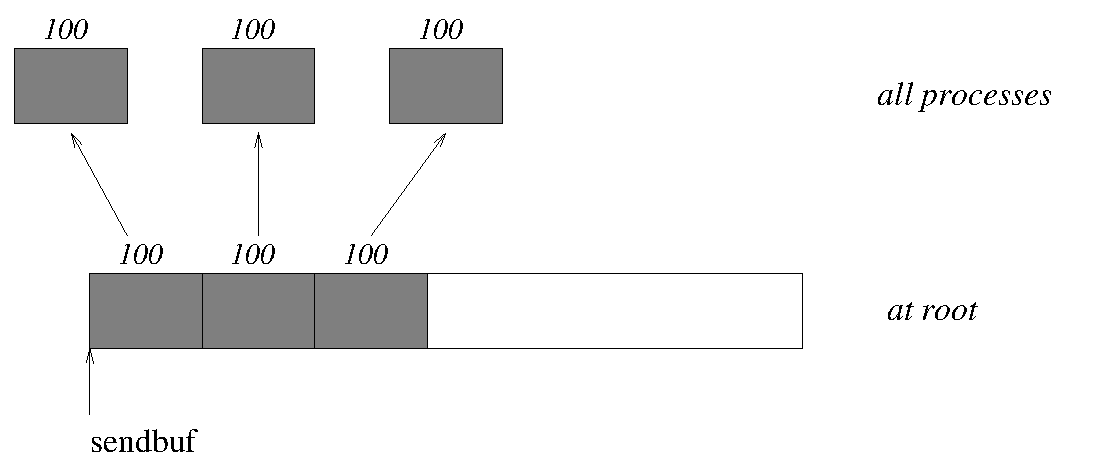
\includegraphics[width=3.50in]{figures/mycoll-fig7}}
  \caption[Scatter example]{The root scatters sets of 100 \code{int}s
    to each \MPI/ process in the group}
  \label{fig-coll-exI}
\end{figure}

\begin{example}
\label{coll-exJ}
\Exindex{C}{Scatterv}{MPI\_Scatterv}%
The reverse of Example~\ref{coll-exC}.
The root scatters sets of 100 \code{int}s to the other \MPI/ processes,
but the sets of 100 are \code{stride int}s apart in the sending buffer.
Requires use of \mpifunc{MPI\_SCATTERV}.
Assume $stride \geq 100$.  See Figure~\ref{fig-coll-exJ}.

%%HEADER
%%LANG: C
%%FRAGMENT
%%SKIPELIPSIS
%%DECL: int stride=100;
%%ENDHEADER
\begin{lstlisting}[language={[MPI]C}]
MPI_Comm comm;
int gsize,*sendbuf;
int root, rbuf[100], i, *displs, *scounts;

...

MPI_Comm_size(comm, &gsize);
sendbuf = (int *)malloc(gsize*stride*sizeof(int));
...
displs = (int *)malloc(gsize*sizeof(int));
scounts = (int *)malloc(gsize*sizeof(int));
for (i=0; i<gsize; ++i) {
    displs[i] = i*stride;
    scounts[i] = 100;
}
MPI_Scatterv(sendbuf, scounts, displs, MPI_INT, rbuf, 100, MPI_INT,
             root, comm);
\end{lstlisting}
\end{example}

\begin{figure}
  \centerline{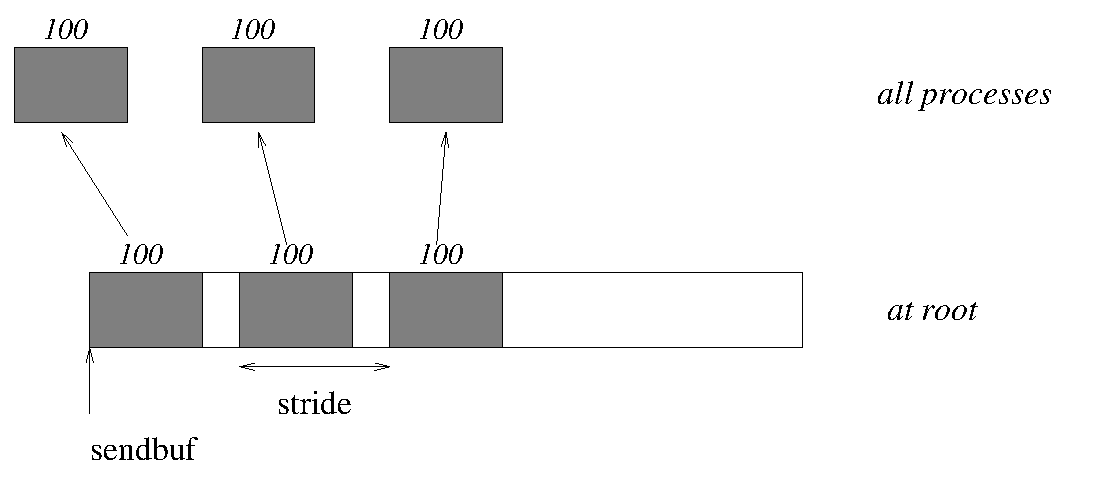
\includegraphics[width=3.50in]{figures/mycoll-fig8}}
  \caption[Scatterv example with strides]{The root scatters sets of
    100 \code{int}s, moving by
  \code{stride int}s from send to send in the scatter}
  \label{fig-coll-exJ}
\end{figure}

\begin{example}
\label{coll-exK}
\Exindex{C}{Scatterv with vector datatype}{MPI\_Scatterv,MPI\_Type\_vector,MPI\_Type\_commit}%
The reverse of Example~\ref{coll-exG}.
We have a varying stride between blocks at sending (root) end,
at the receiving end we receive into the \code{i}-th column of a 100$\times$150
C array.
See Figure~\ref{fig-coll-exK}.

%%HEADER
%%LANG: C
%%FRAGMENT
%%SKIPELIPSIS
%%ENDHEADER
\begin{lstlisting}[language={[MPI]C}]
MPI_Comm comm;
int gsize,recvarray[100][150],*rptr;
int root, *sendbuf, myrank, *stride;
MPI_Datatype rtype;
int i, *displs, *scounts, offset;
...
MPI_Comm_size(comm, &gsize);
MPI_Comm_rank(comm, &myrank);

stride = (int *)malloc(gsize*sizeof(int));
...
/* stride[i] for i = 0 to gsize-1 is set somehow
 * sendbuf comes from elsewhere
 */
...
displs = (int *)malloc(gsize*sizeof(int));
scounts = (int *)malloc(gsize*sizeof(int));
offset = 0;
for (i=0; i<gsize; ++i) {
    displs[i] = offset;
    offset += stride[i];
    scounts[i] = 100 - i;
}
/* Create datatype for the column we are receiving
 */
MPI_Type_vector(100-myrank, 1, 150, MPI_INT, &rtype);
MPI_Type_commit(&rtype);
rptr = &recvarray[0][myrank];
MPI_Scatterv(sendbuf, scounts, displs, MPI_INT, rptr, 1, rtype,
             root, comm);
\end{lstlisting}
\end{example}

\begin{figure}
  \centerline{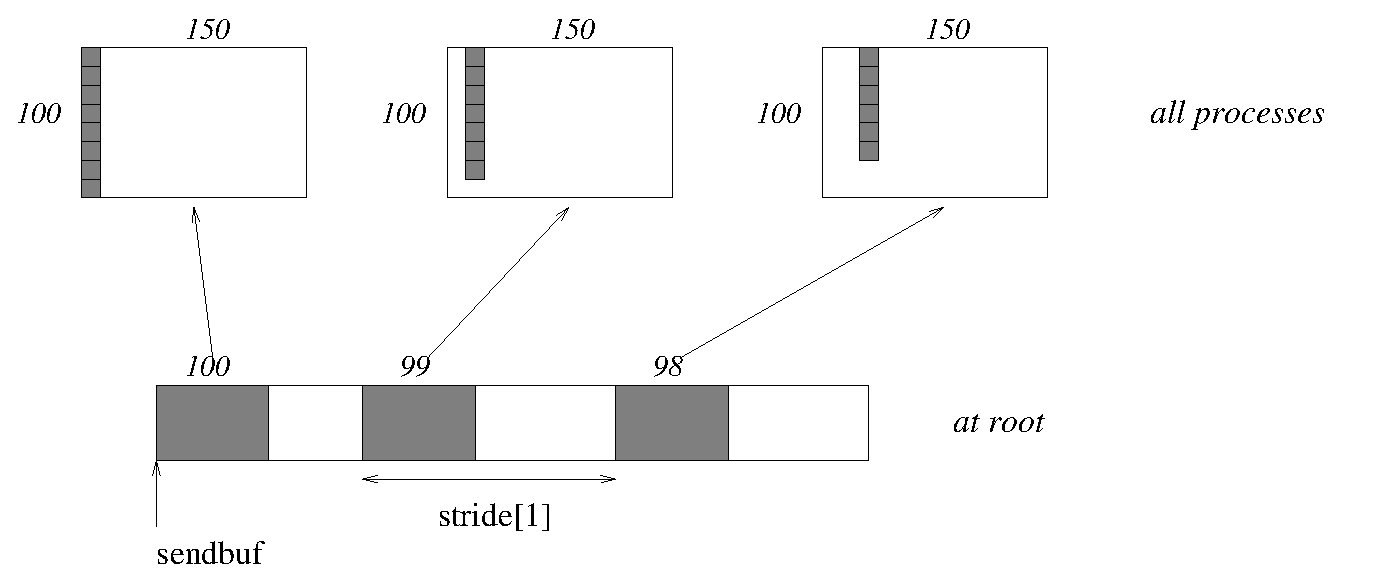
\includegraphics[width=4.00in]{figures/mycoll-fig9}}
  \caption[Scatterv example with different strides and counts]{The root
    scatters blocks of \code{100-i int}s into
    column \code{i} of a 100$\times$150
    C array.  At the sending side, the blocks are \code{stride[i] int}s apart.}
  \label{fig-coll-exK}
\end{figure}

\section{All-Gather}
\mpitermtitleindex{all-gather}
\label{sec:coll-allcast}

\begin{mpi-binding}
    function_name("MPI_Allgather")
    parameter(
        "sendbuf",
        "BUFFER",
        desc=r"starting address of send buffer",
        constant=True,
    )
    parameter(
        "sendcount",
        "POLYXFER_NUM_ELEM_NNI",
        desc=r"number of elements in send buffer",
    )
    parameter("sendtype", "DATATYPE", desc=r"datatype of send buffer elements")
    parameter(
        "recvbuf", "BUFFER", desc=r"address of receive buffer", direction="out"
    )
    parameter(
        "recvcount",
        "POLYXFER_NUM_ELEM_NNI",
        desc=r"number of elements received from any \MPI/ process",
    )
    parameter(
        "recvtype", "DATATYPE", desc=r"datatype of receive buffer elements"
    )
    parameter("comm", "COMMUNICATOR", desc=r"communicator")
\end{mpi-binding}

\mpifunc{MPI\_ALLGATHER} can be thought of as \mpifunc{MPI\_GATHER}, but
where all \MPI/ processes receive the result, instead of just the root.
The block of data sent from the
\mpicode{j}-th
\MPI/ process is received by every \MPI/ process and placed in the
\mpicode{j}-th
block of the buffer \mpiarg{recvbuf}.

The type signature associated with \mpiarg{sendcount, sendtype},
at an \MPI/ process must be equal to the type signature associated with
\mpiarg{recvcount, recvtype} at any other \MPI/ process.

If \mpiarg{comm} is an intra-communicator,
the outcome of a call to \mpifunc{MPI\_ALLGATHER}\mpicode{(...)} is as if
all \MPI/ processes executed \mpicode{n} calls to
%%HEADER
%%LANG: C
%%FRAGMENT
%%DECL: int *sendbuf, *recvbuf, sendcount, recvcount, root;
%%DECL: MPI_Datatype sendtype, recvtype;
%%DECL: MPI_Comm comm;
%%SUBST:\):);
%%SKIPELIPSIS
%%ENDHEADER
\begin{lstlisting}[language={[MPI]C}]
   MPI_Gather(sendbuf,sendcount,sendtype,recvbuf,recvcount,
                                                 recvtype,root,comm)
\end{lstlisting}
for \code{root = 0, ..., n-1}.  The rules for correct usage of
\mpifunc{MPI\_ALLGATHER} can be found in the corresponding rules
for \mpifunc{MPI\_GATHER} (see Section~\ref{sec:coll-gather}).

The ``in place'' option  for intra-communicators is specified by passing the
value
\mpiconstskip{MPI\_IN\_PLACE} to the argument \mpiarg{sendbuf} at all \MPI/ processes.
\mpiarg{sendcount} and \mpiarg{sendtype} are ignored.  Then the input data
of each \MPI/ process is assumed to be in the area where that
\MPI/ process would receive its own contribution to the receive
buffer.

If \mpiarg{comm} is an inter-communicator, then each \MPI/ process
of one group (group A) contributes \mpiarg{sendcount} data items; these
data are concatenated and the result
is stored at each \MPI/ process in the other
group (group B).  Conversely the concatenation of the
contributions of the \MPI/ processes in group B is stored at each \MPI/ process in
group A.   The send buffer arguments in group A must be consistent
with the receive buffer arguments in group B, and vice versa.

\begin{users}
In the inter-communicator case, the communication pattern of \mpifunc{MPI\_ALLGATHER}
need not be symmetric.  The number of items
sent by \MPI/ processes in group A (as specified by the arguments
\mpiarg{sendcount, sendtype} in group A and the arguments
\mpiarg{recvcount, recvtype} in group B), need not equal the number of
items sent by \MPI/ processes in group B (as specified by the arguments
\mpiarg{sendcount, sendtype} in group B and the arguments
\mpiarg{recvcount, recvtype} in group A).  In particular, one can move
data in only one direction by specifying \mpiarg{sendcount}\mpicode{ = 0} for
the communication in the reverse direction.
\end{users}

\begin{mpi-binding}
    function_name("MPI_Allgatherv")
    parameter(
        "sendbuf",
        "BUFFER",
        desc=r"starting address of send buffer",
        constant=True,
    )
    parameter(
        "sendcount",
        "POLYXFER_NUM_ELEM_NNI",
        desc=r"number of elements in send buffer",
    )
    parameter("sendtype", "DATATYPE", desc=r"datatype of send buffer elements")
    parameter(
        "recvbuf", "BUFFER", desc=r"address of receive buffer", direction="out"
    )
    parameter(
        "recvcounts",
        "POLYXFER_NUM_ELEM_NNI",
        desc=(
            r"nonnegative integer array (of length group size) containing "
            r"the number of elements that are received from each \MPI/ process"
        ),
        constant=True,
        length="*",
        suppress="lis_paren",
    )
    parameter(
        "displs",
        "POLYDISPLACEMENT",
        desc=(
            r"integer array (of length group size). Entry \mpicode{i} "
            r"specifies the displacement (relative to \mpiarg{recvbuf}) at "
            r"which to place the incoming data from \MPI/ process \mpicode{i}"
        ),
        constant=True,
        length="*",
        suppress="lis_paren",
    )
    parameter(
        "recvtype", "DATATYPE", desc=r"datatype of receive buffer elements"
    )
    parameter("comm", "COMMUNICATOR", desc=r"communicator")
\end{mpi-binding}

\mpifunc{MPI\_ALLGATHERV} can be thought of as \mpifunc{MPI\_GATHERV}, but
where all processes receive the result, instead of just the root.
The block of data sent from the
\mpicode{j}-th
\MPI/ process is received by every \MPI/ process and placed in the
\mpicode{j}-th
block of the buffer \mpiarg{recvbuf}.
These blocks need not all be the same size.


The type signature associated with \mpiarg{sendcount, sendtype},
at \MPI/ process \mpicode{j} must be equal to the type signature associated with
\mpiarg{recvcounts[j], recvtype} at any other \MPI/ process.

If \mpiarg{comm} is an intra-communicator,
the outcome is as if all \MPI/ processes executed calls to
%%HEADER
%%LANG: C
%%FRAGMENT
%%DECL: int *sendbuf, *recvbuf, sendcount, *recvcounts, *displs, root;
%%DECL: MPI_Datatype sendtype, recvtype;
%%DECL: MPI_Comm comm;
%%SUBST:\):);
%%SKIPELIPSIS
%%ENDHEADER
\begin{lstlisting}[language={[MPI]C}]
    MPI_Gatherv(sendbuf,sendcount,sendtype,recvbuf,recvcounts,displs,
                                                   recvtype,root,comm);
\end{lstlisting}
for \code{root = 0, ..., n-1}.  The rules for correct usage of
\mpifunc{MPI\_ALLGATHERV} can be found in the corresponding rules
for \mpifunc{MPI\_GATHERV} (see Section~\ref{sec:coll-gather}).

The ``in place'' option  for intra-communicators is specified by passing the
value
\mpiconstskip{MPI\_IN\_PLACE} to the argument \mpiarg{sendbuf} at all \MPI/ processes.
In such a case, \mpiarg{sendcount} and \mpiarg{sendtype} are ignored, and the input data
of each \MPI/ process is assumed to be in the area where that
\MPI/ process would receive its own contribution to the receive
buffer.

If \mpiarg{comm} is an inter-communicator, then each \MPI/ process
of one group (group A) contributes \mpiarg{sendcount}
data items; these data are concatenated and the result
is stored at each \MPI/ process in the other
group (group B).  Conversely the concatenation of the
contributions of the \MPI/ processes in group B is stored at each \MPI/ process in
group A.   The send buffer arguments in group A must be consistent
with the receive buffer arguments in group B, and vice versa.

\subsection{Example using \texorpdfstring{\mpifunc{MPI\_ALLGATHER}}{MPI\_ALLGATHER}}
\label{coll:allgather-ex}

The example in this section uses intra-communicators.

\begin{example}
\label{coll-exY}
\Exindex{C}{Allgather}{MPI\_Allgather}%
The all-gather version of Example~\ref{coll-exA}.
Using \mpifunc{MPI\_ALLGATHER}, we will gather 100 \code{int}s from every \MPI/ process in the
group to every \MPI/ process.

%%HEADER
%%LANG: C
%%FRAGMENT
%%SKIPELIPSIS
%%ENDHEADER
\begin{lstlisting}[language={[MPI]C}]
MPI_Comm comm;
int gsize,sendarray[100];
int *rbuf;
...
MPI_Comm_size(comm, &gsize);
rbuf = (int *)malloc(gsize*100*sizeof(int));
MPI_Allgather(sendarray, 100, MPI_INT, rbuf, 100, MPI_INT, comm);
\end{lstlisting}

After the call, every \MPI/ process has the group-wide concatenation of the
sets of data.
\end{example}

\section{All-to-All Scatter/Gather}
\mpitermtitleindex{all-to-all}
\label{sec:coll-alltoall}

\begin{mpi-binding}
    function_name("MPI_Alltoall")
    parameter(
        "sendbuf",
        "BUFFER",
        desc=r"starting address of send buffer",
        constant=True,
    )
    parameter(
        "sendcount",
        "POLYXFER_NUM_ELEM_NNI",
        desc=r"number of elements sent to each \MPI/ process",
    )
    parameter("sendtype", "DATATYPE", desc=r"datatype of send buffer elements")
    parameter(
        "recvbuf", "BUFFER", desc=r"address of receive buffer", direction="out"
    )
    parameter(
        "recvcount",
        "POLYXFER_NUM_ELEM_NNI",
        desc=r"number of elements received from any \MPI/ process",
    )
    parameter(
        "recvtype", "DATATYPE", desc=r"datatype of receive buffer elements"
    )
    parameter("comm", "COMMUNICATOR", desc=r"communicator")
\end{mpi-binding}

\mpifunc{MPI\_ALLTOALL} is an extension of \mpifunc{MPI\_ALLGATHER} to the case
where each \MPI/ process sends distinct data to each of the receivers.
The
\mpicode{j}-th
block sent from \MPI/ process \mpicode{i} is received by \MPI/ process \mpicode{j}
and is placed in the
\mpicode{i}-th
block of \mpiarg{recvbuf}.

The type signature associated with \mpiarg{sendcount, sendtype},
at an \MPI/ process must be equal to the type signature associated with
\mpiarg{recvcount, recvtype} at any other \MPI/ process.
This implies that the amount of data sent must be equal to the
amount of data received, pairwise between every pair of \MPI/ processes.
As usual, however, the type maps may be different.

If \mpiarg{comm} is an intra-communicator,
the outcome is as if each \MPI/ process executed a send to each
\MPI/ process (itself included)
with a call to,
\begin{mpicodeblock}
MPI\_Send(sendbuf+i$\cdot$ sendcount$\cdot$
extent(sendtype),sendcount,sendtype,i, ...),
\end{mpicodeblock}
\noindent and a receive from every other \MPI/ process
with a call to,
\begin{mpicodeblock}
MPI\_Recv(recvbuf+i$\cdot$ recvcount$\cdot$ extent(recvtype),recvcount,recvtype,i,...).
\end{mpicodeblock}

All arguments
on all \MPI/ processes are significant.  The argument \mpiarg{comm}
must have identical values on all \MPI/ processes.

The ``in place'' option for intra-communicators is specified by passing
\mpiconstskip{MPI\_IN\_PLACE} to the argument \mpiarg{sendbuf} at \emph{all} \MPI/ processes.
In such a case, \mpiarg{sendcount} and \mpiarg{sendtype} are ignored.
The data to be sent is taken from the \mpiarg{recvbuf} and replaced by the received data.
Data sent and received must have the same type map as specified by \mpiarg{recvcount} and \mpiarg{recvtype}.

\begin{rationale}
For large \mpifunc{MPI\_ALLTOALL} instances,
allocating both send and receive buffers may consume too much memory.
The ``in place'' option effectively halves the application memory consumption
and is useful in situations where the data to be sent will not be used by the
sending \MPI/ process after the \mpifunc{MPI\_ALLTOALL} exchange (e.g., in parallel
Fast Fourier Transforms).
\end{rationale}

\begin{implementors}
Users may opt to use the ``in place'' option in order to conserve memory.
Quality \MPI/ implementations should thus strive to minimize system buffering.
\end{implementors}

If \mpiarg{comm} is an inter-communicator, then the outcome is as if
each \MPI/ process in group A sends a message to each \MPI/ process in group B,
and vice versa.  The \mpicode{j}-th send buffer of \MPI/ process \mpicode{i} in group A should
be consistent with the \mpicode{i}-th receive buffer of \MPI/ process \mpicode{j} in group B,
and vice versa.

\begin{users}
When a complete exchange is executed in the inter-communicator case, then
the number of data items sent from \MPI/ processes in group A to \MPI/ processes
in group B need not equal the number of items sent in the reverse
direction.  In particular, one can have unidirectional communication
by specifying \mpiarg{sendcount}\mpicode{ = 0} in the reverse direction.
\end{users}


\begin{mpi-binding}
    function_name("MPI_Alltoallv")
    parameter(
        "sendbuf",
        "BUFFER",
        desc=r"starting address of send buffer",
        constant=True,
    )
    parameter(
        "sendcounts",
        "POLYXFER_NUM_ELEM_NNI",
        desc=(
            r"nonnegative integer array (of length group size) specifying "
            r"the number of elements to send to each rank"
        ),
        constant=True,
        length="*",
        suppress="lis_paren",
    )
    parameter(
        "sdispls",
        "POLYDISPLACEMENT",
        desc=(
            r"integer array (of length group size). Entry \mpicode{j} "
            r"specifies the displacement (relative to \mpiarg{sendbuf}) "
            r"from which to take the outgoing data destined for \MPI/ process "
            r"\mpicode{j}"
        ),
        constant=True,
        length="*",
        suppress="lis_paren",
    )
    parameter("sendtype", "DATATYPE", desc=r"datatype of send buffer elements")
    parameter(
        "recvbuf", "BUFFER", desc=r"address of receive buffer", direction="out"
    )
    parameter(
        "recvcounts",
        "POLYXFER_NUM_ELEM_NNI",
        desc=(
            r"nonnegative integer array (of length group size) specifying "
            r"the number of elements that can be received from each rank"
        ),
        constant=True,
        length="*",
        suppress="lis_paren",
    )
    parameter(
        "rdispls",
        "POLYDISPLACEMENT",
        desc=(
            r"integer array (of length group size). Entry \mpicode{i} "
            r"specifies the displacement (relative to \mpiarg{recvbuf}) at "
            r"which to place the incoming data from \MPI/ process \mpicode{i}"
        ),
        constant=True,
        length="*",
        suppress="lis_paren",
    )
    parameter(
        "recvtype", "DATATYPE", desc=r"datatype of receive buffer elements"
    )
    parameter("comm", "COMMUNICATOR", desc=r"communicator")
\end{mpi-binding}

\mpifunc{MPI\_ALLTOALLV} adds flexibility to \mpifunc{MPI\_ALLTOALL} in that
the location of data for the send is specified by \mpiarg{sdispls}
and the location of the placement of the data on the receive side
is specified by \mpiarg{rdispls}.

If \mpiarg{comm} is an intra-communicator, then
the
\mpicode{j}-th
block sent from \MPI/ process \mpicode{i} is received by \MPI/ process \mpicode{j}
and is placed in the
\mpicode{i}-th
block of \mpiarg{recvbuf}.  These blocks need not all have the same size.

The type signature associated with
\mpiarg{sendcounts[j], sendtype} at \MPI/ process \mpicode{i} must be equal
to the type signature
associated with \mpiarg{recvcounts[i], recvtype} at \MPI/ process \mpicode{j}.
This implies that the amount of data sent must be equal to the
amount of data received, pairwise between every pair of \MPI/ processes.
Distinct type maps between sender and receiver are still allowed.

The outcome is as if each \MPI/ process sent a message to every other \MPI/ process
with,
\begin{mpicodeblock}
MPI\_Send(sendbuf+sdispls[i]$\cdot$ extent(sendtype),sendcounts[i],sendtype,i,...),
\end{mpicodeblock}
\noindent and received a message from every other \MPI/ process with
a call to
\begin{mpicodeblock}
MPI\_Recv(recvbuf+rdispls[i]$\cdot$ extent(recvtype),recvcounts[i],recvtype,i,...).
\end{mpicodeblock}

All arguments
on all \MPI/ processes are significant.  The argument \mpiarg{comm}
must have identical values on all \MPI/ processes.

The ``in place'' option for intra-communicators is specified by passing
\mpiconst{MPI\_IN\_PLACE} to the argument \mpiarg{sendbuf} at \emph{all} \MPI/ processes.
In such a case, \mpiarg{sendcounts}, \mpiarg{sdispls} and \mpiarg{sendtype} are ignored.
The data to be sent is taken from the \mpiarg{recvbuf} and replaced by the received data.
Data sent and received must have the same type map as specified by the \mpiarg{recvcounts}
array and the \mpiarg{recvtype}, and is taken from the locations of the receive buffer
specified by \mpiarg{rdispls}.

\begin{users}
Specifying the ``in place'' option (which must be given on all \MPI/ processes)
implies that the same amount and type of data is sent and received between
any two \MPI/ processes in the group of the communicator.
Different pairs of \MPI/ processes can exchange different amounts of data.
Users must ensure that \mpiarg{recvcounts[j]} and \mpiarg{recvtype} on \MPI/ process
\mpicode{i} match \mpiarg{recvcounts[i]} and \mpiarg{recvtype} on \MPI/ process \mpicode{j}.
This symmetric exchange can be useful in applications where the data to be sent will
not be used by the sending \MPI/ process after the \mpifunc{MPI\_ALLTOALLV} exchange.
\end{users}

If \mpiarg{comm} is an inter-communicator, then the outcome is as if
each \MPI/ process in group A sends a message to each \MPI/ process in group B,
and vice versa.  The \mpicode{j}-th send buffer of \MPI/ process \mpicode{i} in group A should
be consistent with the \mpicode{i}-th receive buffer of \MPI/ process \mpicode{j} in group B,
and vice versa.

\begin{rationale}
The definitions of \mpifunc{MPI\_ALLTOALL} and \mpifunc{MPI\_ALLTOALLV} give as much
flexibility as one would achieve by specifying \mpicode{n} independent,
point-to-point communications, with two exceptions: all messages use the same
datatype, and messages are scattered from (or gathered to) sequential
storage.
\end{rationale}

\begin{implementors}
Although the discussion of collective communication in terms of
point-to-point operation implies that each message is transferred directly
from sender to receiver, implementations may use a tree communication
pattern. Messages can be forwarded by intermediate nodes where they
are split (for scatter) or concatenated (for gather), if this
is more efficient.
\end{implementors}

\label{sec:alltoallw}



\begin{mpi-binding}
    function_name("MPI_Alltoallw")
    parameter(
        "sendbuf",
        "BUFFER",
        desc=r"starting address of send buffer",
        constant=True,
    )
    parameter(
        "sendcounts",
        "POLYXFER_NUM_ELEM_NNI",
        desc=(
            r"nonnegative integer array (of length group size) specifying "
            r"the number of elements to send to each rank"
        ),
        constant=True,
        length="*",
        suppress="lis_paren",
    )
    parameter(
        "sdispls",
        "POLYDISPLACEMENT",
        desc=(
            r"integer array (of length group size). Entry \mpicode{j} "
            r"specifies the displacement in bytes (relative to "
            r"\mpiarg{sendbuf}) from which to take the outgoing data "
            r"destined for \MPI/ process \mpicode{j}"
        ),
        constant=True,
        length="*",
    )
    parameter(
        "sendtypes",
        "DATATYPE",
        desc=(
            r"array of datatypes (of length group size). Entry \mpicode{j} "
            r"specifies the type of data to send to \MPI/ process \mpicode{j}"
        ),
        constant=True,
        length="*",
    )
    parameter(
        "recvbuf", "BUFFER", desc=r"address of receive buffer", direction="out"
    )
    parameter(
        "recvcounts",
        "POLYXFER_NUM_ELEM_NNI",
        desc=(
            r"nonnegative integer array (of length group size) specifying "
            r"the number of elements that can be received from each rank"
        ),
        constant=True,
        length="*",
        suppress="lis_paren",
    )
    parameter(
        "rdispls",
        "POLYDISPLACEMENT",
        desc=(
            r"integer array (of length group size). Entry \mpicode{i} "
            r"specifies the displacement in bytes (relative to "
            r"\mpiarg{recvbuf}) at which to place the incoming data from "
            r"\MPI/ process \mpicode{i}"
        ),
        constant=True,
        length="*",
    )
    parameter(
        "recvtypes",
        "DATATYPE",
        desc=(
            r"array of datatypes (of length group size). Entry \mpicode{i} "
            r"specifies the type of data received from \MPI/ process \mpicode{i}"
        ),
        constant=True,
        length="*",
    )
    parameter("comm", "COMMUNICATOR", desc=r"communicator")
\end{mpi-binding}

\mpifunc{MPI\_ALLTOALLW}
is the most general form of complete exchange.
Like \mpifunc{MPI\_TYPE\_CREATE\_STRUCT}, the most general type constructor,
\mpifunc{MPI\_ALLTOALLW} allows separate specification of count,
displacement and datatype.  In addition, to allow maximum flexibility,
the displacement of blocks within the send and receive buffers is
specified in bytes.

If \mpiarg{comm} is an intra-communicator, then
the \mpicode{j}-th block sent from \MPI/ process \mpicode{i} is received by \MPI/ process
\mpicode{j} and is placed in the \mpicode{i}-th block of \mpiarg{recvbuf}.
These blocks need not all have the same size.

The type signature associated with
\mpiarg{sendcounts[j], sendtypes[j]} at \MPI/ process \mpicode{i} must be equal
to the type signature
associated with \mpiarg{recvcounts[i], recvtypes[i]} at \MPI/ process \mpicode{j}.
This implies that the amount of data sent must be equal to the
amount of data received, pairwise between every pair of \MPI/ processes.
Distinct type maps between sender and receiver are still allowed.

The outcome is as if each \MPI/ process sent a message to every other \MPI/ process with
\begin{mpicodeblock}
MPI\_Send(sendbuf+sdispls[i],sendcounts[i],sendtypes[i] ,i,...),
\end{mpicodeblock}
\noindent and received a message from every other \MPI/ process with a call to
\begin{mpicodeblock}
MPI\_Recv(recvbuf+rdispls[i],recvcounts[i],recvtypes[i] ,i,...).
\end{mpicodeblock}

All arguments on all \MPI/ processes are significant.  The argument
\mpiarg{comm} must describe the same communicator on all \MPI/ processes.

Like for \mpifunc{MPI\_ALLTOALLV}, the ``in place'' option for intra-communicators
is specified by passing \mpiconstskip{MPI\_IN\_PLACE} to the argument \mpiarg{sendbuf}
at \emph{all} \MPI/ processes.
In such a case, \mpiarg{sendcounts}, \mpiarg{sdispls} and \mpiarg{sendtypes} are ignored.
The data to be sent is taken from the \mpiarg{recvbuf} and replaced by the received data.
Data sent and received must have the same type map as specified by the \mpiarg{recvcounts}
and \mpiarg{recvtypes} arrays, and is taken from the locations of the receive buffer
specified by \mpiarg{rdispls}.

If \mpiarg{comm} is an inter-communicator, then the outcome is as if
each \MPI/ process in group A sends a message to each \MPI/ process in group B,
and vice versa.  The \mpicode{j}-th send buffer of \MPI/ process \mpicode{i} in group A should
be consistent with the \mpicode{i}-th receive buffer of \MPI/ process \mpicode{j} in group B,
and vice versa.


\begin{rationale}
The \mpifunc{MPI\_ALLTOALLW} function generalizes several \MPI/ functions by
carefully selecting the input arguments.  For example, by making all but one
\MPI/ process have \mpicode{sendcounts[i] = 0}, 
this achieves what one would expect from an \mpifuncskip{MPI\_SCATTERW}, if such a function existed, which is equivalent to an \mpifunc{MPI\_SCATTERV} with the blocks not all needing to have the same datatypes. 
\end{rationale}

\section{Global Reduction Operations}
\mpitermtitleindex{reduction operations}
\label{global-reduce}

The functions in this section perform a global reduce operation
(for example sum, maximum, and logical and) across
all members of a group.
The reduction operation can be either one of a predefined list of
operations, or a user-defined operation.
The global reduction functions come in several flavors: a reduce that
returns the result of the reduction
to one member of a group,
an all-reduce that
returns this result
to all members of a group,
and
two
scan (parallel prefix)
operations.
In addition, a reduce-scatter operation combines the
functionality of a reduce and of a scatter operation.

\subsection{Reduce}
\mpitermtitleindex{reduce}
\label{subsec:coll-reduce}

\cdeclindex{MPI\_Op}%
\begin{mpi-binding}
    function_name("MPI_Reduce")
    parameter("sendbuf", "BUFFER", desc=r"address of send buffer", constant=True)
    parameter(
        "recvbuf",
        "BUFFER",
        desc=r"address of receive buffer",
        direction="out",
        root_only=True,
    )
    parameter(
        "count",
        "POLYXFER_NUM_ELEM_NNI",
        desc=r"number of elements in send buffer",
    )
    parameter(
        "datatype", "DATATYPE", desc=r"datatype of elements of send buffer"
    )
    parameter("op", "OPERATION", desc=r"reduce operation")
    parameter("root", "RANK", desc=r"rank of the root")
    parameter("comm", "COMMUNICATOR", desc=r"communicator")
\end{mpi-binding}

If \mpiarg{comm} is an intra-communicator,
\mpifunc{MPI\_REDUCE} combines the elements provided
in the input buffer of each \MPI/ process in the
group, using the operation \mpiarg{op}, and returns the combined value in
the output buffer of the \MPI/ process with rank \mpiarg{root}.
The input buffer is defined by the arguments \mpiarg{sendbuf},
\mpiarg{count} and \mpiarg{datatype}; the output buffer is defined by
the arguments \mpiarg{recvbuf}, \mpiarg{count} and \mpiarg{datatype};
both have the same number of elements, with the same type.
The routine is called by all group members using the same arguments
for \mpiarg{count, datatype, op, root} and \mpiarg{comm}.
Thus, all \MPI/ processes provide input buffers of the
same length, with elements of the same type as the output buffer at the root.
Each \MPI/ process can provide one element, or a sequence of elements,
in which case the
combine operation is executed element-wise on each entry of the sequence.
For example, if the operation is \mpiconst{MPI\_MAX} and the send buffer
contains two elements that are floating point numbers (\mpiarg{count} = 2 and
\mpiarg{datatype} = \type{MPI\_FLOAT}), then $\mpicode{recvbuf(1)} =
global \max (\mpicode{sendbuf(1)})$ and $\mpicode{recvbuf(2)} = global \max ( \mpicode{sendbuf(2)})$.

Section~\ref{coll-predefined-op}, lists the set of predefined operations
provided by \MPI/. That section also enumerates
the datatypes
to which each operation can be applied.

In addition, users may define their own operations that can be
overloaded to operate on several datatypes, either basic or derived.
This is further explained in Section~\ref{subsec:coll-user-ops}.

The operation \mpiarg{op} is always assumed to be
associative.  All predefined operations are also assumed to be
commutative.  Users may define operations that are assumed to be
associative, but not commutative.  The ``canonical'' evaluation order
of a reduction is determined by the ranks of the \MPI/ processes in the
group.  However, the implementation can take
advantage of associativity, or associativity and commutativity
in order to change the order of evaluation.
This may change the result of the reduction for operations that are not
strictly associative and commutative, such as floating point addition.


\begin{implementors}
It is strongly recommended that \mpifunc{MPI\_REDUCE} be implemented so
that the same result be obtained
whenever the function is applied on the same arguments,
appearing in the same order.  Note that this may
prevent optimizations that take
advantage of the physical location of ranks.
\end{implementors}

\begin{users}
Some applications may not be able to ignore the nonassociative nature of
floating-point operations or may use user-defined operations
(see Section~\ref{subsec:coll-user-ops}) that require a special reduction
order and cannot be treated as associative.
Such applications should enforce the order of evaluation explicitly.
For example, in the case of operations that require a strict left-to-right
(or right-to-left) evaluation order, this could be done by gathering all
operands at a single \MPI/ process (e.g., with \mpifunc{MPI\_GATHER}), applying the
reduction operation in the desired order (e.g., with \mpifunc{MPI\_REDUCE\_LOCAL}),
and if needed, broadcast or scatter the result to the other \MPI/ processes
(e.g., with \mpifunc{MPI\_BCAST}).
\end{users}

The \mpiarg{datatype} argument of \mpifunc{MPI\_REDUCE} must be
compatible with
\mpishortarg{op}.
Predefined operators work only with
the \MPI/ types listed in Section~\ref{coll-predefined-op} and
Section~\ref{coll-minloc-maxloc}.  Furthermore, the
\mpiarg{datatype} and \mpiarg{op} given for predefined operators
must be the same on all \MPI/ processes.

Note that it is possible for users to supply different user-defined operations
to \mpifunc{MPI\_REDUCE} in each \MPI/ process.  \MPI/ does not define which
operations are used on which operands in this case.
User-defined operators may operate on general, derived datatypes.
In this case, each argument that
the reduce operation is applied to is one element described by such a datatype,
which may contain several basic values.
This is further explained in Section~\ref{subsec:coll-user-ops}.
\begin{users}
  Users should make no assumptions about how \mpifunc{MPI\_REDUCE} is
  implemented.  It is safest to ensure that the same function is passed to
  \mpifunc{MPI\_REDUCE} by each \MPI/ process.
\end{users}

Overlapping datatypes are permitted in ``send'' buffers.
Overlapping datatypes in ``receive'' buffers are erroneous
and may give unpredictable results.

The ``in place'' option  for intra-communicators is specified by passing the
value
\mpiconstskip{MPI\_IN\_PLACE} to the argument \mpiarg{sendbuf} at the root.
In such a case, the input data is taken at the root from the receive buffer,
where it will be replaced by the output data.


If \mpiarg{comm} is an inter-communicator, then the call involves all
\MPI/ processes in the inter-communicator, but with one group (group A) defining the
root.  All \MPI/ processes in the other group (group B) pass the same value
in argument
\mpiarg{root}, which is the rank of the root in group A.  The root
passes the value \mpiconstskip{MPI\_ROOT} in \mpiarg{root}.
All other \MPI/ processes in group A pass the value \mpiconst{MPI\_PROC\_NULL} in
\mpiarg{root}.
Only send buffer arguments are significant in group B and only receive
buffer arguments are significant at the root.

\subsection{Predefined Reduction Operations}
\mpitermtitleindexsubmain{predefined}{reduction operations}
\label{coll-predefined-op}

The following predefined operations are supplied for \mpifunc{MPI\_REDUCE}
and related functions \mpifunc{MPI\_ALLREDUCE},
\mpifunc{MPI\_REDUCE\_SCATTER\_BLOCK}, \mpifunc{MPI\_REDUCE\_SCATTER},
\mpifunc{MPI\_SCAN},
\mpifunc{MPI\_EXSCAN}, all
nonblocking variants of those (see Section~\ref{sec:nbcoll}), and
\mpifunc{MPI\_REDUCE\_LOCAL}.  These operations are invoked by placing
the following in \mpiarg{op}.

\begin{constlist}
\noconstitem{Name}{Meaning}
\noconstitem{}{ }
\constmainitem{MPI\_MAX}{maximum}
\constmainitem{MPI\_MIN}{minimum}
\constmainitem{MPI\_SUM}{sum}
\constmainitem{MPI\_PROD}{product}
\constmainitem{MPI\_LAND}{logical and }
\constmainitem{MPI\_BAND}{bit-wise and }
\constmainitem{MPI\_LOR}{logical or }
\constmainitem{MPI\_BOR}{bit-wise or }
\constmainitem{MPI\_LXOR}{logical exclusive or (xor)}
\constmainitem{MPI\_BXOR}{bit-wise exclusive or (xor)}
\constmainitem{MPI\_MAXLOC}{max value and location}
\constmainitem{MPI\_MINLOC}{min value and location}
\end{constlist}

The two operations \mpiconst{MPI\_MINLOC} and \mpiconst{MPI\_MAXLOC} are
discussed separately in Section~\ref{coll-minloc-maxloc}.
For the other predefined operations,
we enumerate below the allowed combinations of \mpiarg{op} and
\mpiarg{datatype} arguments.
First, define groups of \MPI/ basic datatypes
in the following way.

% Use constlist for the list format, but just use item for the entries
\begin{constlist}
\noconstitem{C integer:}{\type{MPI\_INT}, \type{MPI\_LONG}, \type{MPI\_SHORT},}
\noconstitem{}{\type{MPI\_UNSIGNED\_SHORT}, \type{MPI\_UNSIGNED},}
\noconstitem{}{\type{MPI\_UNSIGNED\_LONG},}
\noconstitem{}{\type{MPI\_LONG\_LONG\_INT},}
\noconstitem{}{\type{MPI\_LONG\_LONG} (as synonym),}
\noconstitem{}{\type{MPI\_UNSIGNED\_LONG\_LONG},}
\noconstitem{}{\type{MPI\_SIGNED\_CHAR},}
\noconstitem{}{\type{MPI\_UNSIGNED\_CHAR},}
\noconstitem{}{\type{MPI\_INT8\_T}, \type{MPI\_INT16\_T},}
\noconstitem{}{\type{MPI\_INT32\_T}, \type{MPI\_INT64\_T},}
\noconstitem{}{\type{MPI\_UINT8\_T}, \type{MPI\_UINT16\_T},}
\noconstitem{}{\type{MPI\_UINT32\_T}, and \type{MPI\_UINT64\_T}}
\noconstitem{Fortran integer:}{\type{MPI\_INTEGER}}
\noconstitem{}{and handles returned from}
\noconstitem{}{\mpifunc{MPI\_TYPE\_CREATE\_F90\_INTEGER}}
\noconstitem{}{and, if available, \type{MPI\_INTEGER1},}
\noconstitem{}{\type{MPI\_INTEGER2}, \type{MPI\_INTEGER4},}
\noconstitem{}{\type{MPI\_INTEGER8}, and \type{MPI\_INTEGER16}}
\noconstitem{Floating point:}{\type{MPI\_FLOAT}, \type{MPI\_DOUBLE}, \type{MPI\_REAL},}
\noconstitem{}{\type{MPI\_DOUBLE\_PRECISION},}
\noconstitem{}{\type{MPI\_LONG\_DOUBLE},}
\noconstitem{}{and handles returned from }
\noconstitem{}{\mpifunc{MPI\_TYPE\_CREATE\_F90\_REAL}}
\noconstitem{}{and, if available, \type{MPI\_REAL2},}
\noconstitem{}{\type{MPI\_REAL4}, \type{MPI\_REAL8}, and \type{MPI\_REAL16}}
\noconstitem{Logical:}{\type{MPI\_LOGICAL}, \type{MPI\_C\_BOOL},}
\noconstitem{}{\type{MPI\_CXX\_BOOL},}
\noconstitem{}{and, if available, \type{MPI\_LOGICAL1},}
\noconstitem{}{\type{MPI\_LOGICAL2}, \type{MPI\_LOGICAL4},}
\noconstitem{}{\type{MPI\_LOGICAL8}, and \type{MPI\_LOGICAL16},}
\noconstitem{Complex:}{\type{MPI\_COMPLEX}, \type{MPI\_C\_COMPLEX},}
\noconstitem{}{\type{MPI\_C\_FLOAT\_COMPLEX} (as synonym),}
\noconstitem{}{\type{MPI\_C\_DOUBLE\_COMPLEX},}
\noconstitem{}{\type{MPI\_C\_LONG\_DOUBLE\_COMPLEX},}
\noconstitem{}{\type{MPI\_CXX\_FLOAT\_COMPLEX},}
\noconstitem{}{\type{MPI\_CXX\_DOUBLE\_COMPLEX},}
\noconstitem{}{\type{MPI\_CXX\_LONG\_DOUBLE\_COMPLEX},}
\noconstitem{}{and handles returned from }
\noconstitem{}{\mpifunc{MPI\_TYPE\_CREATE\_F90\_COMPLEX}}
\noconstitem{}{and, if available, \type{MPI\_DOUBLE\_COMPLEX},}
\noconstitem{}{\type{MPI\_COMPLEX4}, \type{MPI\_COMPLEX8},}
\noconstitem{}{\type{MPI\_COMPLEX16}, and \type{MPI\_COMPLEX32}}
\noconstitem{Byte:}{\type{MPI\_BYTE}}
\noconstitem{Multi-language types:}{\type{MPI\_AINT}, \type{MPI\_OFFSET}, and \type{MPI\_COUNT}}
\end{constlist}

Now, the valid datatypes for each operation are specified below.

\begin{constlist}[170pt]
\noconstitem{Op}{Allowed Types}
\noconstitem{}{ }
\constitemtwo{MPI\_MAX}{MPI\_MIN}{C integer, Fortran integer, Floating point,}
\noconstitem{}{Multi-language types}
\constitemtwo{MPI\_SUM}{MPI\_PROD}{C integer, Fortran integer, Floating point, Complex,}
\noconstitem{}{Multi-language types}
\constitemthree{MPI\_LAND}{MPI\_LOR}{MPI\_LXOR}{C integer, Logical}
\constitemthree{MPI\_BAND}{MPI\_BOR}{MPI\_BXOR}{C integer, Fortran integer, Byte, Multi\hyphen/language types}
\end{constlist}

These operations together with all listed
datatypes are valid in all supported programming languages, see also
Reduce Operations in
Section~\ref{subsec:mpiopaqueobjects}.

The following examples use intra-communicators.

\begin{example}
\label{coll-exblas1}
\Exindex{Fortran}{Reduction}{MPI\_Reduce}%
A routine that computes
the dot product of two vectors that are distributed across a
group of \MPI/ processes and returns the answer at node zero.

%%HEADER
%%LANG: FORTRAN90
%%SKIPELIPSIS
%%ENDHEADER
\begin{lstlisting}[language={[MPI]Fortran}]
SUBROUTINE PAR_BLAS1(m, a, b, c, comm)
USE MPI
REAL a(m), b(m)       ! local slice of array
REAL c                ! result (at node zero)
REAL sum
INTEGER m, comm, i, ierr

! local sum
sum = 0.0
DO i = 1, m
   sum = sum + a(i)*b(i)
END DO

! global sum
CALL MPI_REDUCE(sum, c, 1, MPI_REAL, MPI_SUM, 0, comm, ierr)
RETURN
END
\end{lstlisting}
\end{example}

\begin{example}
\label{coll-exblas2}
\Exindex{Fortran}{Reduction of a vector}{MPI\_Reduce}%
A routine that computes
the product of a vector and an array that are distributed across a
group of \MPI/ processes and returns the answer at node zero.

%%HEADER
%%LANG: FORTRAN90
%%SKIPELIPSIS
%%ENDHEADER
\begin{lstlisting}[language={[MPI]Fortran}]
SUBROUTINE PAR_BLAS2(m, n, a, b, c, comm)
USE MPI
REAL a(m), b(m,n)    ! local slice of array
REAL c(n)            ! result
REAL sum(n)
INTEGER m, n, comm, i, j, ierr

! local sum
DO j=1,n
   sum(j) = 0.0
   DO i=1,m
      sum(j) = sum(j) + a(i)*b(i,j)
   END DO
END DO

! global sum
CALL MPI_REDUCE(sum, c, n, MPI_REAL, MPI_SUM, 0, comm, ierr)

! return result at node zero (and garbage at the other nodes)
RETURN
END
\end{lstlisting}
\end{example}

\subsection{Signed Characters and Reductions}

The types \type{MPI\_SIGNED\_CHAR} and \type{MPI\_UNSIGNED\_CHAR} can be
used in reduction operations. \type{MPI\_CHAR},
\type{MPI\_WCHAR}, and \type{MPI\_CHARACTER} (which represent printable
characters) cannot be used in reduction operations.
In a heterogeneous environment,
\type{MPI\_CHAR}, \type{MPI\_WCHAR}, and \type{MPI\_CHARACTER}
will be translated so as to preserve the printable character, whereas
\type{MPI\_SIGNED\_CHAR} and \type{MPI\_UNSIGNED\_CHAR} will be
translated so as to preserve the integer value.

\begin{users}
The types \type{MPI\_CHAR}, \type{MPI\_WCHAR}, and \type{MPI\_CHARACTER} are intended for
characters, and so will be translated to preserve the printable
representation, rather than the integer value, if sent between machines with
different character codes.  The types \type{MPI\_SIGNED\_CHAR} and
\type{MPI\_UNSIGNED\_CHAR} should be used in C if the integer value
should be preserved.
\end{users}



\subsection{MINLOC and MAXLOC}
\label{coll-minloc-maxloc}

The operator \mpiconst{MPI\_MINLOC} is used to compute
a global minimum and also
an index attached to the minimum value.
\mpiconst{MPI\_MAXLOC} similarly computes a global maximum and index.
One application of these is to compute a global minimum (maximum) and the
rank of the \MPI/ process containing this value.

The operation that defines \mpiconst{MPI\_MAXLOC} is:

\[
\left( \begin{array}{c} u \\ i \end{array} \right)
\circ
\left( \begin{array}{c} v \\ j \end{array} \right)
=
\left( \begin{array}{c} w \\ k \end{array} \right)
\]
where
\[
w = \max (u,v)
\]
and
\[
k = \left\{ \begin{array}{ll}
    i & \mbox{if $u > v$} \\
    \min(i,j) & \mbox{if $u=v$} \\
    j & \mbox{if $u < v$}
\end{array}
\right.
\]

\mpiconst{MPI\_MINLOC} is defined similarly:

\[
\left( \begin{array}{c} u \\ i \end{array} \right)
\circ
\left( \begin{array}{c} v \\ j \end{array} \right)
=
\left( \begin{array}{c} w \\ k \end{array} \right)
\]
where
\[
w = \min (u,v)
\]
and
\[
k = \left\{ \begin{array}{ll}
    i & \mbox{if $u < v$} \\
    \min(i,j) & \mbox{if $u=v$} \\
    j & \mbox{if $u > v$}
\end{array}
\right.
\]

Both operations are associative and commutative.
Note that if \mpiconst{MPI\_MAXLOC}
is applied to reduce a sequence of pairs
$(u_0, 0), (u_1, 1) , \ldots, (u_{n-1} , n-1)$, then the value
returned is $(u , r)$, where $u = \max_i u_i$ and $r$ is the index of
the first global maximum in the sequence.  Thus, if each \MPI/ process
supplies a value and its rank within the group, then a reduce
operation with \mpiarg{op} = \mpiconst{MPI\_MAXLOC} will return the
maximum value and the rank of the first \MPI/ process with that value.
Similarly, \mpiconst{MPI\_MINLOC} can be used to return a minimum and its
index.
More generally, \mpiconst{MPI\_MINLOC} computes a \emph{lexicographic
minimum}, where elements are ordered according to the first component
of each pair, and ties are resolved according to the second component.

The reduce operation is defined to operate on arguments that
consist of a pair: value and index.
For both Fortran and C, types are provided to describe the pair.
The potentially mixed-type nature of such arguments
is a problem in older versions of Fortran.  The problem is circumvented there by
having the \MPI/-provided type consist of a pair of the same type as
value, and coercing the index to this type also.  In C, the \MPI/-provided
pair type has distinct types and the index is an integer type. For
named predefined pair types in C the index is of type \code{int}.
For unnamed predefined pair types, other integer types are allowed as
index instead.
To use pair types with distinct value and index in Fortran, these types need to be defined using \code{BIND(C)} and be equivalent to the corresponding C struct.


In order to use \mpiconst{MPI\_MINLOC} and \mpiconst{MPI\_MAXLOC} in a
reduce operation, one must provide a \mpiarg{datatype} argument
that represents a pair (value and index).  \MPI/ provides
nine
such named predefined datatypes as well as the function \mpifunc{MPI\_TYPE\_GET\_VALUE\_INDEX} to query named and unnamed predefined types using value type and index type.  The operations \mpiconst{MPI\_MAXLOC} and
\mpiconst{MPI\_MINLOC} can be used with each of the following named datatypes.
\begin{constlist}
\noconstitem{Fortran:}{ }
\noconstitem{Name}{Description}
\mpidtypemainitem{MPI\_2REAL}{pair of \ftype{REAL}s}
\mpidtypemainitem{MPI\_2DOUBLE\_PRECISION}{pair of \ftype{DOUBLE PRECISION} variables}
\mpidtypemainitem{MPI\_2INTEGER}{pair of \ftype{INTEGER}s}
\end{constlist}
\begin{constlist}%
\noconstitem{C:}{ }
\noconstitem{Name}{Description}
\mpidtypemainitem{MPI\_FLOAT\_INT}{\ctype{float} and \ctype{int}}
\mpidtypemainitem{MPI\_DOUBLE\_INT}{\ctype{double} and \ctype{int}}
\mpidtypemainitem{MPI\_LONG\_INT}{\ctype{long} and \ctype{int}}
\mpidtypemainitem{MPI\_2INT}{pair of \ctype{int} }
\mpidtypemainitem{MPI\_SHORT\_INT}{\ctype{short} and \ctype{int} }
\mpidtypemainitem{MPI\_LONG\_DOUBLE\_INT}{\ctype{long double} and \ctype{int} }
\end{constlist}

The datatype \type{MPI\_2REAL} is \emph{as if} defined by the following
(see Section~\ref{sec:pt2pt-datatype}).

%%HEADER
%%LANG: FORTRAN08
%%FRAGMENT
%%DECL: TYPE(MPI_DATATYPE) tworeal
%%DECL: INTEGER ierror
%%SUBST:MPI_2REAL:tworeal
%%ENDHEADER
\begin{lstlisting}[language={[MPI]Fortran}]
call MPI_Type_contiguous(2, MPI_REAL, MPI_2REAL, ierror)
\end{lstlisting}

Similar statements apply for \type{MPI\_2INTEGER},
\type{MPI\_2DOUBLE\_PRECISION}, and \type{MPI\_2INT}.

The datatype \type{MPI\_SHORT\_INT} is \emph{as if} defined by the
following sequence of instructions.
% Note that this is in language-independent form, not C or Fortran
%%HEADER
%%LANG: C
%%FRAGMENT
%%TOP: #include <stddef.h>
%%DECL: MPI_Datatype type[2]; int block[2];
%%DECL: MPI_Aint disp[2];
%%DECL: MPI_Datatype rshortint;
%%SUBST:MPI_SHORT_INT:rshortint
%%ENDHEADER
\begin{lstlisting}[language={[MPI]C}]
struct mystruct {
    short val;
    int rank;
};
type[0] = MPI_SHORT;
type[1] = MPI_INT;
disp[0] = 0;
disp[1] = offsetof(struct mystruct, rank);
block[0] = 1;
block[1] = 1;
MPI_Type_create_struct(2, block, disp, type, &MPI_SHORT_INT);
MPI_Type_commit(&MPI_SHORT_INT);
\end{lstlisting}
Similar statements apply for \type{MPI\_FLOAT\_INT}, \type{MPI\_LONG\_INT}
and \type{MPI\_DOUBLE\_INT}.

\begin{mpi-binding}
    function_name("MPI_Type_get_value_index")
    parameter("value_type", "DATATYPE", desc=r"datatype of the value in pair")
    parameter("index_type", "DATATYPE", desc=r"datatype of the index in pair")
    parameter(
        "pair_type",
        "DATATYPE",
        desc=r"datatype of the value-index pair",
        direction="out"
    )
\end{mpi-binding}

\mpifunc{MPI\_TYPE\_GET\_VALUE\_INDEX} returns a handle to a predefined datatype suitable for the use with \mpiconst{MPI\_MINLOC} and \mpiconst{MPI\_MAXLOC} if such a predefined type exists.
If the provided combination of \mpiarg{value\_type} and \mpiarg{index\_type} does not match a predefined pair datatype (named or unnamed), the function will set \mpiarg{pair\_type} to \mpiconst{MPI\_DATATYPE\_NULL} and return \mpiconst{MPI\_SUCCESS}.
The returned type is not a duplicate.
This type cannot be freed.
Types supported by the underlying compiler for which the operators \mpiconst{MPI\_MIN} and \mpiconst{MPI\_MAX} are defined in Section~\ref{coll-predefined-op} are acceptable value types.
Integer types supported by the underlying compiler are acceptable index types.

\begin{sloppy}
\begin{users}
    Note that a named type handle returned by \mpifunc{MPI\_TYPE\_GET\_VALUE\_INDEX} will yield the combiner value \mpiconst{MPI\_COMBINER\_NAMED} when queried with \mpifunc{MPI\_TYPE\_GET\_ENVELOPE} to ensure backward compatibility to existing behavior, whereas all unnamed type handles returned by \mpifunc{MPI\_TYPE\_GET\_VALUE\_INDEX} will yield the combiner value \mpiconst{MPI\_COMBINER\_VALUE\_INDEX} when queried with \mpifunc{MPI\_TYPE\_GET\_ENVELOPE}.
    There is no observable difference between the named constant value used via its symbol name or via \mpifunc{MPI\_TYPE\_GET\_VALUE\_INDEX}.
    Code evaluating the combiner of type handles returned from \mpifunc{MPI\_TYPE\_GET\_VALUE\_INDEX} must therefore handle both \mpiconst{MPI\_COMBINER\_NAMED} and \mpiconst{MPI\_COMBINER\_VALUE\_INDEX}.
\end{users}
\end{sloppy}

\begin{example}
\label{coll-value-index-c}
\Exindex{C}{Retrieving an unnamed predefined value-index handle}{MPI\_TYPE\_GET\_VALUE\_INDEX}
An unnamed predefined value-index type is retrieved for use with the corresponding C struct.
If the requested value-index pair does not exist as a predefined type \mpiconst{MPI\_DATATYPE\_NULL} is returned.

%%HEADER
%%LANG: C
%%FRAGMENT
%%TOP: #include <stddef.h>
%%TOP: #include <stdint.h>
%%ENDHEADER
\begin{lstlisting}[language={[MPI]C}]
    struct mystruct {
        double val;
        uint64_t index;
    };

    MPI_Datatype dtype;
    MPI_Type_get_value_index(MPI_DOUBLE, MPI_UINT64_T, &dtype);

    if (dtype == MPI_DATATYPE_NULL) {
        // Handling for unsupported value-index type
    }
\end{lstlisting}
\end{example}

\begin{users}
    Implementations may apply certain optimizations to operations on compound types with equally sized value and index types. Such optimizations may not be applicable to operations on compound types where value and index type are of different size.
\end{users}

The following examples use intra-communicators.

\begin{example}
\label{coll-exminlocC}
\Exindex{C}{Reduction with maxloc}{MPI\_Reduce}%
Each \MPI/ process has an array of 30 \ctype{double}s, in C.  For each
of the 30 locations, compute the value and rank of the \MPI/ process containing
the largest value.

%%HEADER
%%LANG: C
%%DECL: MPI_Comm comm;
%%FRAGMENT
%%SKIPELIPSIS
%%ENDHEADER
\begin{lstlisting}[language={[MPI]C}]
...
/* each MPI process has an array of 30 double: ain[30]
 */
double ain[30], aout[30];
int  ind[30];
struct {
    double val;
    int   rank;
} in[30], out[30];
int i, myrank, root;

MPI_Comm_rank(comm, &myrank);
for (i=0; i<30; ++i) {
    in[i].val = ain[i];
    in[i].rank = myrank;
}
MPI_Reduce(in, out, 30, MPI_DOUBLE_INT, MPI_MAXLOC, root, comm);
/* At this point, the answer resides on root MPI process
 */
if (myrank == root) {
    /* read ranks out
     */
    for (i=0; i<30; ++i) {
        aout[i] = out[i].val;
        ind[i] = out[i].rank;
    }
}
\end{lstlisting}
\end{example}



\begin{example}
\label{coll-exminlocF}
\Exindex{Fortran}{Reduction with maxloc}{MPI\_Reduce}%
Same example, in Fortran.

%%HEADER
%%LANG: FORTRAN90
%%FRAGMENT
%%DECL: INTEGER COMM
%%SKIPELIPSIS
%%ENDHEADER
\begin{lstlisting}[language={[MPInoinout]Fortran}]
...
! each process has an array of 30 double: ain(30)

DOUBLE PRECISION ain(30), aout(30)
INTEGER ind(30)
DOUBLE PRECISION in(2,30), out(2,30)
INTEGER i, myrank, root, ierr

CALL MPI_COMM_RANK(comm, myrank, ierr)
DO i=1,30
   in(1,i) = ain(i)
   in(2,i) = myrank    ! myrank is coerced to a double
END DO

CALL MPI_REDUCE(in, out, 30, MPI_2DOUBLE_PRECISION, MPI_MAXLOC, root,&
                comm, ierr)
! At this point, the answer resides on root MPI process

IF (myrank .EQ. root) THEN
   ! read ranks out
   DO i=1,30
      aout(i) = out(1,i)
      ind(i) = out(2,i)  ! rank is coerced back to an integer
   END DO
END IF
\end{lstlisting}
\end{example}




\begin{example}
\label{coll-exminlocC2}
\Exindex{C}{Reduction with minloc}{MPI\_Reduce}%
Each \MPI/ process has a nonempty array of values.
Find the minimum global value, the rank of the \MPI/ process that holds it
and its index on this \MPI/ process.

%%HEADER
%%LANG: C
%%FRAGMENT
%%DECL: int i, root;
%%DECL: MPI_Comm comm;
%%SKIPELIPSIS
%%TAIL: if (minrank<0 || minindex<0 || minval<0)abort();
%%ENDHEADER
\begin{lstlisting}[language={[MPI]C}]
#define  LEN   1000

float val[LEN];        /* local array of values */
int count;             /* local number of values */
int myrank, minrank, minindex;
float minval;

struct {
    float value;
    int   index;
} in, out;

/* local minloc */
in.value = val[0];
in.index = 0;
for (i=1; i < count; i++) {
    if (in.value > val[i]) {
        in.value = val[i];
        in.index = i;
    }
}
/* global minloc */
MPI_Comm_rank(comm, &myrank);
in.index = myrank*LEN + in.index;
MPI_Reduce(&in, &out, 1, MPI_FLOAT_INT, MPI_MINLOC, root, comm);

/* At this point, the answer resides on the root */
if (myrank == root) {
    /* read answer out */
    minval = out.value;
    minrank = out.index / LEN;
    minindex = out.index % LEN;
}
\end{lstlisting}
\end{example}

\begin{rationale}
The definition of \mpiconst{MPI\_MINLOC} and \mpiconst{MPI\_MAXLOC} given
here has the advantage that it does not require any special-case
handling of these two operations: they are handled like any other
reduce operation.  By assigning a value other than \code{myrank} to the \code{in.index} field, a programmer can provide a different definition
of \mpiconst{MPI\_MAXLOC} and \mpiconst{MPI\_MINLOC}, if so desired.
The disadvantage is that values and indices have to be first
interleaved, and that indices and values have to be coerced to the
same type, in Fortran.
\end{rationale}

\subsection{User-Defined Reduction Operations}
\mpitermtitleindexsubmain{user-defined}{reduction operations}
\label{subsec:coll-user-ops}

% Exceptions with MPI_Op_create:
%  - Due to a POLYFUNCTION parameter, it will be embiggened,
%    but in Fortran, explicit name with _c must be produced (no function overloading).
%    Therefore, "not_abstract_interface()" is needed (see also MPI_Register_datarep and MPI_CONVERSION_FN_NULL).
\cdeclmainindex{MPI\_Op}\cdeclmainindex{TYPE(MPI\_Op)}%
\begin{mpi-binding}
    function_name("MPI_Op_create")
    not_abstract_interface()

    parameter(
        "user_fn",
        "POLYFUNCTION",
        desc=r"user defined function",
        func_type="MPI_User_function",
    )
    parameter(
        "commute",
        "LOGICAL",
        desc=r"\mpicode{true} if commutative; \mpicode{false} otherwise.",
        suppress="lis_paren",
    )
    parameter(
        "op", "OPERATION", desc=r"operation", direction="out",
    )
\end{mpi-binding}

\mpifunc{MPI\_OP\_CREATE} binds a user-defined reduction operation
to an \mpishortarg{op} handle that can subsequently be used in
\mpifunc{MPI\_REDUCE}, \mpifunc{MPI\_ALLREDUCE},
\mpifunc{MPI\_REDUCE\_SCATTER},
\mpifunc{MPI\_REDUCE\_SCATTER\_BLOCK},
\mpifunc{MPI\_SCAN}, \mpifunc{MPI\_EXSCAN}, all nonblocking and persistent variants of
those (see Section~\ref{sec:nbcoll} and Section~\ref{sec:pcoll}), and \mpifunc{MPI\_REDUCE\_LOCAL}.
The user-defined operation is assumed to be associative.
If \mpiarg{commute} $=$ \mpicode{true}, then the operation should be both
commutative and associative. If  \mpiarg{commute} $=$ \mpicode{false},
then the order of operands is fixed and is defined to be in ascending, process
rank order, beginning with \MPI/ process with rank \mpicode{0} in the communicator \mpiarg{comm}.  The order of evaluation can be
changed, talking advantage of the associativity of the operation.  If
\mpiarg{commute} $=$ \mpicode{true} then the order of evaluation can be changed,
taking advantage of commutativity and associativity.

In Fortran when using \code{USE mpi\_f08}, the large count variant shall
be called explicitly as \MPIBCfunc{MPI\_Op\_create\_c} (i.e., with suffix ``\code{\_c}''\mpitermindex{\_c@\code{\_c}})
because interface polymorphism cannot be used to differentiate between the
two different user callback prototypes despite their different type
signatures.

The argument \mpiarg{user\_fn} is the user-defined function, which must have the
following four arguments: \mpiarg{invec}, \mpiarg{inoutvec}, \mpiarg{len}, and
\mpiarg{datatype}.

\mpicallbackskip{MPI\_USER\_FUNCTION} also supports large count types in
separate additional \MPI/ callback function prototype declarations in C (suffixed with the ``\code{\_c}'') and
in Fortran when using \code{USE mpi\_f08}.

The ISO C prototypes for the functions are the following.

\begin{mpi-binding}
    callback()
    return_type("NOTHING")
    no_lis_binding()
    no_render("f08, f90")

    function_name("MPI_User_function", "USER_FUNCTION")

    parameter("invec", "C_BUFFER4", length="len")
    parameter("inoutvec", "C_BUFFER4", length="len")
    parameter("len", "POLYXFER_NUM_ELEM", pointer=True)
    parameter("datatype", "DATATYPE", pointer=True)

    no_ierror()
\end{mpi-binding}

The Fortran declarations of the user-defined function \mpiarg{user\_fn} appear
below.

\begin{mpi-binding}
    render("mpi_user_function", "f08")
\end{mpi-binding}
\begin{mpi-binding}
    render("mpi_user_function", "f90")
\end{mpi-binding}

The \mpiarg{datatype} argument
is a handle to the datatype that was passed into the call
to \mpifunc{MPI\_REDUCE}.
The user reduce function should be written such that the following
holds:
Let \mpicode{u[0], $\ldots$ , u[len-1]} be the \mpiarg{len} elements in the
communication buffer described by the arguments \mpiarg{invec, len}
and \mpiarg{datatype} when the function is invoked;
let \mpicode{v[0], $\ldots$ , v[len-1]} be \mpiarg{len} elements in the
communication buffer described by the arguments \mpiarg{inoutvec, len}
and \mpiarg{datatype} when the function is invoked;
let \mpicode{w[0], $\ldots$ , w[len-1]} be  \mpiarg{len} elements in the
communication buffer described by the arguments \mpiarg{inoutvec, len}
and \mpiarg{datatype} when the function returns;
then \mpicode{w[i] = u[i]$\circ$v[i]}, for \mpicode{i=0 , $\ldots$ , len-1},
where $\circ$ is the reduce operation that the function computes.

Informally, we can think of
\mpiarg{invec} and \mpiarg{inoutvec} as arrays of \mpiarg{len} elements that
\mpiarg{user\_fn}
is combining.  The result of the reduction over-writes values in
\mpiarg{inoutvec}, hence the name.  Each invocation of the function results in
the pointwise evaluation of the reduce operator on \mpiarg{len}
elements:
i.e., the function returns in \mpiarg{inoutvec[i]} the value
$\mpicode{invec[i]} \circ \mpicode{inoutvec[i]}$, for $\mpicode{i=0, \ldots , count-1}$,
where $\circ$ is the combining operation computed by the function.

\begin{rationale}
The
\mpiarg{len}
argument allows
\mpifunc{MPI\_REDUCE} to avoid calling the function for each element
in the input buffer.  Rather, the system can choose to apply
the function to chunks of input.  In C, it is passed in as
a reference for reasons of compatibility with Fortran.

By internally comparing the value of the \mpiarg{datatype} argument to
known, global handles,
it is possible to overload the use of a single user-defined function
for several, different datatypes.
\end{rationale}

When calling any reduction or prefix scan \MPI/ procedure with a
user-defined \MPI/ operator, the type of the \mpiarg{count} parameter in
the call to the reduction or prefix scan \MPI/ procedure does not need
to be identical to the type of the \mpiarg{len} parameter in the user
function associated with the user-defined \MPI/ operator.  If the
\mpiarg{count} parameter has a type of \ctype{int} in C or
\ftype{INTEGER} in Fortran and the \mpiarg{len} parameter has a type
of \mpidtype{MPI\_COUNT}, then \MPI/ will perform the appropriate widening
type conversion of the \mpiarg{len} parameter.  If the \mpiarg{count}
parameter has a type of \type{MPI\_COUNT} and the \mpiarg{len}
parameter has a type of \ctype{int} in C or \ftype{INTEGER} in
Fortran, then \MPI/ will perform the appropriate narrowing type
conversion of the \mpiarg{len} parameter.  If this narrowing
conversion would result in truncation of the \mpiarg{len} value, then
\MPI/ will call the user function multiple times with a sequence of
values for \mpiarg{len} that sum to the value of \mpiarg{count}.

General datatypes may be passed to the user function.
However, use of datatypes that are not contiguous is likely to lead to
inefficiencies.

No \MPI/ communication function may be called inside the user function.
\mpifunc{MPI\_ABORT} may be called inside the
function in case of an error.

\begin{users}
Suppose one defines a library of user-defined reduce
functions that are overloaded: the \mpiarg{datatype} argument is used
to select the right execution path at each invocation, according to
the types of the operands.
The user-defined reduce function cannot ``decode'' the
\mpiarg{datatype} argument that it is passed, and cannot identify,
by itself, the correspondence between the datatype handles and the datatype
they represent.  This correspondence was established when the datatypes
were created.  Before the library is used, a library initialization
preamble must be executed.  This preamble code will define the
datatypes that are used by the library, and store handles to these
datatypes in global, static variables that are shared by the user code and the
library code.

The Fortran version of \mpifunc{MPI\_REDUCE} will invoke a user-defined reduce
function using the Fortran calling conventions and will pass a Fortran-type
datatype argument;  the C version will use C calling convention and the C
representation of a datatype handle.  Users who plan to mix languages should
define their reduction functions accordingly.
\end{users}


\begin{implementors}
We outline below a naive and inefficient implementation of \mpifunc{MPI\_REDUCE}
not
supporting the ``in place'' option and only valid for intra\hyphen/communicators.

%%HEADER
%%LANG: C
%%FRAGMENT
%%SUBST: rank-1,\.\.\.:rank-1,0,comm,&status
%%SUBST: rank\+1, \.\.\.:rank+1, 0, comm
%%SUBST: groupsize-1,\.\.\.:groupsize-1,0,comm
%%SUBST: root, \.\.\.:root, 0, comm
%%SUBST: groupsize-1 \.\.\.:groupsize-1
%%DECL: MPI_Comm comm;
%%DECL: int groupsize, rank, count, *tempbuf, *sendbuf, *recvbuf, root;
%%DECL: MPI_Datatype datatype;
%%DECL: MPI_Request req;
%%DECL: MPI_Status status;
%%DECL: void User_reduce(void *, void *, int, MPI_Datatype);
%%ENDHEADER
\begin{lstlisting}[language={[MPI]C}]
MPI_Comm_size(comm, &groupsize);
MPI_Comm_rank(comm, &rank);
if (rank > 0) {
    MPI_Recv(tempbuf, count, datatype, rank-1,...);
    User_reduce(tempbuf, sendbuf, count, datatype);
}
if (rank < groupsize-1) {
    MPI_Send(sendbuf, count, datatype, rank+1, ...);
}
/* answer now resides in MPI process groupsize-1 ...
 * now send to root
 */
if (rank == root) {
    MPI_Irecv(recvbuf, count, datatype, groupsize-1,..., &req);
}
if (rank == groupsize-1) {
    MPI_Send(sendbuf, count, datatype, root, ...);
}
if (rank == root) {
    MPI_Wait(&req, &status);
}
\end{lstlisting}

The reduction computation proceeds, sequentially, from \MPI/ process with rank \code{0}
to \MPI/ process with rank
\gb\code{groupsize-1}.
This order is chosen so as to respect
the order of a possibly noncommutative operator defined by the
function \code{User\_reduce()}.
A more efficient implementation is achieved by taking advantage
of associativity and
using a logarithmic tree reduction.  Commutativity can be used
to advantage, for those cases in which the \mpiarg{commute} argument
to \mpifunc{MPI\_OP\_CREATE} is true.  Also, the amount of temporary buffer
space required can be reduced, and communication can be pipelined with
computation, by transferring and reducing the elements in chunks of
size \code{len} $<$\code{count}.

The predefined reduce operations can be implemented as a library of
user-defined operations.  However, better performance might be
achieved if \mpifunc{MPI\_REDUCE} handles these functions as a special
case.
\end{implementors}

\cdeclindex{MPI\_Op}%
\begin{mpi-binding}
    function_name("MPI_Op_free")
    parameter("op", "OPERATION", desc=r"operation", direction="inout")
\end{mpi-binding}

Marks a user-defined reduction operation for deallocation and sets
\mpiarg{op} to \mpiconstmain{MPI\_OP\_NULL}.

\subsubsection{Example of User-Defined Reduce}
\label{coll-user-reduce-example}

The example in this section uses an intra-communicator.

\begin{example}
\label{coll-exX}
\Exindex{C}{Reduction with user-defined op}{MPI\_Reduce,MPI\_Op\_create}%
Compute the product of an array of complex numbers, in C.
% Note - this should be broken into two separate lstlistings
% (the "and to call it" should not be within lstlsting)
% The definition of the user-defined function avoids compiler warnings
% since the user-defined function should use the void * parameters.
%%HEADER
%%LANG: C
%%SUBST:it\.\.\.:it---
%%SUBST:\.\.\.:void test(MPI_Comm comm,int root){
%%TAIL:}
%%ENDHEADER
\begin{lstlisting}[language={[MPI]C}]
typedef struct {
    double real,imag;
} Complex;

/* the user-defined function
 */
void myProd(void *inP, void *inoutP, int *len, MPI_Datatype *dptr)
{
    int i;
    Complex c;
    Complex *in = (Complex *)inP, *inout = (Complex *)inoutP;

    for (i=0; i< *len; ++i) {
        c.real = inout->real*in->real -
                   inout->imag*in->imag;
        c.imag = inout->real*in->imag +
                   inout->imag*in->real;
        *inout = c;
        in++; inout++;
    }
}

/* and, to call it...
 */
...

    /* each MPI process has an array of 100 Complexes
     */
    Complex a[100], answer[100];
    MPI_Op myOp;
    MPI_Datatype ctype;

    /* explain to MPI how type Complex is defined
     */
    MPI_Type_contiguous(2, MPI_DOUBLE, &ctype);
    MPI_Type_commit(&ctype);
    /* create the complex-product user-op
     */
    MPI_Op_create(myProd, 1, &myOp);

    MPI_Reduce(a, answer, 100, ctype, myOp, root, comm);

    /* At this point, the answer, which consists of 100 Complexes,
     * resides on root MPI process
     */
\end{lstlisting}
\end{example}

\begin{example}
\label{coll-exX-fortran}
\Exindex{Fortran}{Defining a user function}{MPI\_Reduce,MPI\_Op\_create}%
\mpicallbackindex{MPI\_User\_function}%
How to use the \code{mpi\_f08} interface of the Fortran \mpifcallback{MPI\_User\_function}.
%%HEADER
%%LANG: FORTRAN08
%%ENDHEADER
\begin{lstlisting}[language={[MPI08]Fortran}]
subroutine my_user_function(invec, inoutvec, len, dtype)   bind(c)
   use, intrinsic :: iso_c_binding, only : c_ptr, c_f_pointer
   use mpi_f08
   type(c_ptr), value :: invec, inoutvec
   integer :: len
   type(MPI_Datatype) :: dtype
   real, pointer :: invec_r(:), inoutvec_r(:)
   if (dtype == MPI_REAL) then
      call c_f_pointer(invec, invec_r, (/ len /))
      call c_f_pointer(inoutvec, inoutvec_r, (/ len /))
      inoutvec_r = invec_r + inoutvec_r
   end if
end subroutine
\end{lstlisting}
\end{example}

\subsection{All-Reduce}
\mpitermtitleindex{all-reduce}
\label{subsec:coll-all-reduce}

\MPI/ includes
a variant
of the reduce operations
where the result is returned to all \MPI/ processes in
a
group.
\MPI/ requires that all \MPI/ processes
from the same group
participating in these operations
receive identical results.

\cdeclindex{MPI\_Op}%
\begin{mpi-binding}
    function_name("MPI_Allreduce")
    parameter(
        "sendbuf",
        "BUFFER",
        desc=r"starting address of send buffer",
        constant=True,
    )
    parameter(
        "recvbuf",
        "BUFFER",
        desc=r"starting address of receive buffer",
        direction="out",
    )
    parameter(
        "count",
        "POLYXFER_NUM_ELEM_NNI",
        desc=r"number of elements in send buffer",
    )
    parameter(
        "datatype", "DATATYPE", desc=r"datatype of elements of send buffer"
    )
    parameter("op", "OPERATION", desc=r"operation")
    parameter("comm", "COMMUNICATOR", desc=r"communicator")
\end{mpi-binding}

If \mpiarg{comm} is an intra-communicator,
\mpifunc{MPI\_ALLREDUCE} behaves the
same as \mpifunc{MPI\_REDUCE} except that the result
appears in the receive buffer of all the group members.

\begin{implementors}
The all-reduce operations can be implemented as a reduce, followed by a
broadcast.  However, a direct implementation can lead to better performance.
\end{implementors}

The ``in place'' option  for intra-communicators is specified by passing the
value \mpiconstskip{MPI\_IN\_PLACE} to the argument \mpiarg{sendbuf}
at all processes.
In this case,
the input data is taken at each \MPI/ process from the receive buffer,
where it will be replaced by the output data.

If \mpiarg{comm} is an inter-communicator, then the result of the reduction
of the data provided by \MPI/ processes in group A is stored at each \MPI/ process
in group B, and vice versa.
Both groups should
provide \mpiarg{count} and \mpiarg{datatype} arguments that specify the same type
signature.

The following example uses an intra-communicator.

\begin{example}
\label{coll-exallblas2}
\Exindex{Fortran}{Allreduce of a vector}{MPI\_Allreduce}%
A routine that computes
the product of a vector and an array that are distributed across a
group of \MPI/ processes and returns the answer at all nodes (see also
Example~\ref{coll-exblas2}).

%%HEADER
%%LANG: FORTRAN90
%%SKIPELIPSIS
%%ENDHEADER
\begin{lstlisting}[language={[MPI]Fortran}]
SUBROUTINE PAR_BLAS2(m, n, a, b, c, comm)
USE MPI
REAL a(m), b(m,n)    ! local slice of array
REAL c(n)            ! result
REAL sum(n)
INTEGER m, n, comm, i, j, ierr

! local sum
DO j=1,n
   sum(j) = 0.0
   DO i=1,m
      sum(j) = sum(j) + a(i)*b(i,j)
   END DO
END DO

! global sum
CALL MPI_ALLREDUCE(sum, c, n, MPI_REAL, MPI_SUM, comm, ierr)

! return result at all nodes
RETURN
END
\end{lstlisting}
\end{example}

\subsection{\texorpdfstring{\MPI/}{MPI} Process-Local Reduction}
\mpitermtitleindex{reduction operations!process-local}
\label{subsec:coll-process-local-reduction} % Sect. 5.9.7 p.173 NEWsection

The functions in this section are of importance to library implementors
who may want to implement special reduction patterns that are otherwise
not easily covered by the standard \MPI/ operations.

The following function applies a reduction operator to local arguments.

\cdeclindex{MPI\_Op}%
\begin{mpi-binding}
    function_name("MPI_Reduce_local")
    parameter("inbuf", "BUFFER", desc=r"input buffer", constant=True)
    parameter(
        "inoutbuf",
        "BUFFER",
        desc=r"combined input and output buffer",
        direction="inout",
    )
    parameter(
        "count",
        "POLYXFER_NUM_ELEM_NNI",
        desc=r"number of elements in \mpiarg{inbuf} and \mpiarg{inoutbuf} buffers",
    )
    parameter(
        "datatype",
        "DATATYPE",
        desc=r"datatype of elements of \mpiarg{inbuf} and \mpiarg{inoutbuf} buffers",
    )
    parameter("op", "OPERATION", desc=r"operation")
\end{mpi-binding}

The function applies the operation given by \mpiarg{op} element-wise to the elements of
\mpiarg{inbuf} and \mpiarg{inoutbuf} with the result stored element-wise in \mpiarg{inoutbuf},
as explained for user-defined operations in Section~\ref{subsec:coll-user-ops}.
Both \mpiarg{inbuf} and \mpiarg{inoutbuf} (input as well as result) have the same number
of elements given by \mpiarg{count} and the same datatype given by \mpiarg{datatype}.
The \mpiconstskip{MPI\_IN\_PLACE} option is not allowed.

\cdeclindex{MPI\_Op}%
\begin{mpi-binding}
    function_name("MPI_Op_commutative")
    parameter("op", "OPERATION", desc=r"operation")
    parameter(
        "commute",
        "LOGICAL",
        desc=r"\mpicode{true} if \mpiarg{op} is commutative, \mpicode{false} otherwise",
        direction="out",
    )
\end{mpi-binding}

Reduction operations can be queried for their commutativity using \mpifunc{MPI\_OP\_COMMUTATIVE}.

\section{Reduce-Scatter}
\mpitermtitleindex{reduce-scatter}
\label{sec:coll-reduce-scatter}

\MPI/ includes variants of the reduce operations where the result is scattered
to all \MPI/ processes in a group on return.
One variant scatters equal-sized blocks to all \MPI/ processes,
while another variant scatters blocks that may vary in size for each \MPI/ process.

\subsection{\texorpdfstring{\mpifunc{MPI\_REDUCE\_SCATTER\_BLOCK}}{MPI\_REDUCE\_SCATTER\_BLOCK}}
\label{subsec:coll-reduce-scatter-block} % Sect. 5.10.1 p.174 NEWsection

\cdeclindex{MPI\_Op}%
\begin{mpi-binding}
    function_name("MPI_Reduce_scatter_block")
    parameter(
        "sendbuf",
        "BUFFER",
        desc=r"starting address of send buffer",
        constant=True,
    )
    parameter(
        "recvbuf",
        "BUFFER",
        desc=r"starting address of receive buffer",
        direction="out",
    )
    parameter(
        "recvcount", "POLYXFER_NUM_ELEM_NNI", desc=r"element count per block"
    )
    parameter(
        "datatype",
        "DATATYPE",
        desc=r"datatype of elements of send and receive buffers",
    )
    parameter("op", "OPERATION", desc=r"operation")
    parameter("comm", "COMMUNICATOR", desc=r"communicator")
\end{mpi-binding}

If \mpiarg{comm} is an intra-communicator, \mpifunc{MPI\_REDUCE\_SCATTER\_BLOCK}
first performs a global, element-wise reduction on vectors of \mpiarg{count}\mpicode{ = n*}\mpiarg{recvcount}
elements in the send buffers defined by \mpiarg{sendbuf}, \mpiarg{count} and \mpiarg{datatype},
using the operation \mpiarg{op}, where \mpicode{n} is the number of \MPI/ processes in the group of \mpiarg{comm}.
The routine is called by all group members using the same arguments for \mpiarg{recvcount},
\mpiarg{datatype}, \mpiarg{op} and \mpiarg{comm}.
The resulting vector is treated as \mpicode{n} consecutive blocks of \mpiarg{recvcount} elements
that are scattered to the \MPI/ processes of the group.
The \mpicode{i}-th block is sent to \MPI/ process \mpicode{i} and stored in the receive buffer defined by
\mpiarg{recvbuf}, \mpiarg{recvcount}, and \mpiarg{datatype}.

\begin{implementors}
The \mpifunc{MPI\_REDUCE\_SCATTER\_BLOCK} routine is functionally equivalent to
an \mpifunc{MPI\_REDUCE} collective operation with \mpiarg{count} equal to \mpiarg{recvcount*\mpicode{n}},
followed by an \mpifunc{MPI\_SCATTER} with \mpiarg{sendcount} equal to \mpiarg{recvcount}.
However, a direct implementation may run faster.
\end{implementors}

The ``in place'' option for intra-communicators is specified by passing \mpiconstskip{MPI\_IN\_PLACE}
in the \mpiarg{sendbuf} argument on \emph{all} \MPI/ processes.
In this case, the input data is taken from the receive buffer.

If \mpiarg{comm} is an inter-communicator, then the result of the reduction of the data provided
by \MPI/ processes in one group (group A) is scattered among \MPI/ processes in the other group (group B) and vice versa.
Within each group, all \MPI/ processes provide the same value for the \mpiarg{recvcount} argument,
and provide input vectors of \mpiarg{count}\mpicode{ = n*}\mpiarg{recvcount} elements stored in the send buffers,
where \mpicode{n} is the size of the group.
The number of elements \mpiarg{count} must be the same for the two groups.
The resulting vector from the other group is scattered in blocks of \mpiarg{recvcount}
elements among the \MPI/ processes in the group.

\begin{rationale}
The last restriction is needed so that the length of the send buffer of one group can be
determined by the local \mpiarg{recvcount} argument of the other group.
Otherwise, communication is needed to figure out how many elements are reduced.
\end{rationale}


\subsection{\texorpdfstring{\mpifunc{MPI\_REDUCE\_SCATTER}}{MPI\_REDUCE\_SCATTER}}
\label{subsec:coll-reduce-scatter} % Sect. 5.10.1 p.174 NEWsection

\mpifunc{MPI\_REDUCE\_SCATTER} extends the functionality of \mpifunc{MPI\_REDUCE\_SCATTER\_BLOCK}
such that the scattered blocks can vary in size.
Block sizes are determined by the \mpiarg{recvcounts} array,
such that the \mpicode{i}-th block contains \mpiarg{recvcounts[i]} elements.

\cdeclindex{MPI\_Op}%
\begin{mpi-binding}
    function_name("MPI_Reduce_scatter")
    parameter(
        "sendbuf",
        "BUFFER",
        desc=r"starting address of send buffer",
        constant=True,
    )
    parameter(
        "recvbuf",
        "BUFFER",
        desc=r"starting address of receive buffer",
        direction="out",
    )
    parameter(
        "recvcounts",
        "POLYXFER_NUM_ELEM_NNI",
        desc=(
            r"nonnegative integer array (of length group size) specifying "
            r"the number of elements of the result distributed to each "
            r"\MPI/ process."
        ),
        constant=True,
        length="*",
        suppress="lis_paren",
    )
    parameter(
        "datatype",
        "DATATYPE",
        desc=r"datatype of elements of send and receive buffers",
    )
    parameter("op", "OPERATION", desc=r"operation")
    parameter("comm", "COMMUNICATOR", desc=r"communicator")
\end{mpi-binding}

If \mpiarg{comm} is an intra-communicator,
\mpifunc{MPI\_REDUCE\_SCATTER} first
performs a global, element-wise reduction on vectors of
\gb{$\mpicode{count} = \sum_{i=0}^{n-1} \mpicode{recvcounts[i]}$} elements in the send
buffers defined by \mpiarg{sendbuf}, \mpiarg{count} and
\mpiarg{datatype}, using the operation \mpiarg{op}, where \mpicode{n} is the number of
\MPI/ processes in the group of \mpiarg{comm}. The routine is called by all group
members using the same arguments for \mpiarg{recvcounts},
\mpiarg{datatype}, \mpiarg{op} and \mpiarg{comm}.
The resulting vector is treated as \mpicode{n} consecutive blocks where the number
of elements of the \mpicode{i}-th block is \mpiarg{recvcounts[i]}. The blocks are scattered
to the \MPI/ processes of the group. The \mpicode{i}-th block
is sent to \MPI/ process \mpicode{i} and stored in the
receive buffer defined by \mpiarg{recvbuf, recvcounts[i]} and
\mpiarg{datatype}.


\begin{implementors}
The \mpifunc{MPI\_REDUCE\_SCATTER}
routine is functionally equivalent to
an
\mpifunc{MPI\_REDUCE}
collective
operation
with \mpiarg{count} equal to
the sum of \mpiarg{recvcounts[i]} followed by
\mpifunc{MPI\_SCATTERV} with \mpiarg{sendcounts} equal to \mpiarg{recvcounts}.
However, a direct implementation may run faster.
\end{implementors}

The ``in place'' option  for intra-communicators is specified by passing
\mpiconstskip{MPI\_IN\_PLACE} in
the \mpiarg{sendbuf} argument.
In this case, the input data is taken from the receive
buffer. It is not required to specify the ``in
place'' option on all \MPI/ processes, since the \MPI/ processes for which
\mpiarg{recvcounts[i]}\mpicode{ =0} may not have allocated a receive buffer.

If \mpiarg{comm} is an inter-communicator, then the result of the reduction
of the data provided by \MPI/ processes in one
group (group A) is scattered among \MPI/ processes in
the other group (group B), and vice
versa.  Within each group, all \MPI/ processes provide the same
\mpiarg{recvcounts} argument, and provide input vectors of \gb{$\mpicode{count} = \sum_{i=0}^{n-1} \mpicode{recvcounts[i]}$}
elements stored in the send buffers, where \mpicode{n} is the size of the group.
The resulting vector from the other group is scattered in blocks of
\mpiarg{recvcounts[i]} elements among the \MPI/ processes in the group. The number of
elements \mpiarg{count} must be the same for the two groups.

\begin{rationale}
The last restriction is needed so that the length of the send
buffer can be determined by the sum of the local \mpiarg{recvcounts} entries.
Otherwise, communication is needed to figure out how many elements
are reduced.
\end{rationale}

\section{Scan}
\mpitermtitleindexmainsub{reduction operations}{scan}
\label{sec:coll-scan}
\subsection{Inclusive Scan}
\mpitermtitleindexsubmain{inclusive}{scan}
\label{subsec:coll-scan}
\cdeclindex{MPI\_Op}%
\begin{mpi-binding}
    function_name("MPI_Scan")
    parameter(
        "sendbuf",
        "BUFFER",
        desc=r"starting address of send buffer",
        constant=True,
    )
    parameter(
        "recvbuf",
        "BUFFER",
        desc=r"starting address of receive buffer",
        direction="out",
    )
    parameter(
        "count",
        "POLYXFER_NUM_ELEM_NNI",
        desc=r"number of elements in input buffer",
    )
    parameter(
        "datatype", "DATATYPE", desc=r"datatype of elements of input buffer"
    )
    parameter("op", "OPERATION", desc=r"operation")
    parameter("comm", "COMMUNICATOR", desc=r"communicator")
\end{mpi-binding}

If \mpiarg{comm} is an intra-communicator,
\mpifunc{MPI\_SCAN} is used to perform a prefix reduction
on data distributed across the group.
The operation returns, in the receive buffer of the \MPI/ process with rank
\mpicode{i}, the
reduction of the values in the send buffers of \MPI/ processes with ranks
\mpicode{0,$\ldots$,i} (inclusive).  The routine is called by all
group members using the same arguments for \mpiarg{count}, \mpiarg{datatype},
\mpiarg{op} and \mpiarg{comm},
except that for user-defined operations, the same rules apply as for
\mpifunc{MPI\_REDUCE}. The type of operations supported, their semantics,
and the constraints on send and receive buffers are as for
\mpifunc{MPI\_REDUCE}.

The ``in place'' option  for intra-communicators is specified by passing
\mpiconstskip{MPI\_IN\_PLACE}
in the \mpiarg{sendbuf} argument.  In this case, the input data is
taken from the receive buffer, and replaced by the output data.

This operation is invalid for inter-communicators.

\subsection{Exclusive Scan}
\label{subsec:coll-exscan}
\label{coll-exscan} % Sect. 5.11.2 p.175 newlabel

\cdeclindex{MPI\_Op}%
\begin{mpi-binding}
    function_name("MPI_Exscan")
    parameter(
        "sendbuf",
        "BUFFER",
        desc=r"starting address of send buffer",
        constant=True,
    )
    parameter(
        "recvbuf",
        "BUFFER",
        desc=r"starting address of receive buffer",
        direction="out",
    )
    parameter(
        "count",
        "POLYXFER_NUM_ELEM_NNI",
        desc=r"number of elements in input buffer",
    )
    parameter(
        "datatype", "DATATYPE", desc=r"datatype of elements of input buffer"
    )
    parameter("op", "OPERATION", desc=r"operation")
    parameter("comm", "COMMUNICATOR", desc=r"intra-communicator")
\end{mpi-binding}

If \mpiarg{comm} is an intra-communicator,
\mpifunc{MPI\_EXSCAN} is used to perform a prefix reduction on data distributed
across the group.
The value in \mpiarg{recvbuf} on the \MPI/ process with rank \mpicode{0} is undefined, and \mpiarg{recvbuf} is not signficant on that \MPI/ process.
The value in \mpiarg{recvbuf} on the \MPI/ process with rank \mpicode{1} is defined as
the value in \mpiarg{sendbuf} on the \MPI/ process with rank \mpicode{0}.
For \MPI/ processes with rank $ i > 1 $, the operation returns, in the
receive buffer of the
\MPI/ process with rank $i$, the reduction of the values in the send buffers
of \MPI/ processes with ranks $0,\ldots,i-1$ (inclusive).
The routine is called by all group members using
the same arguments for \mpiarg{count}, \mpiarg{datatype}, \mpiarg{op}
and \mpiarg{comm}, except that for
user-defined operations, the same rules apply as for
\mpifunc{MPI\_REDUCE}. The type of operations supported, their semantics,
and the constraints on send and receive buffers, are as for
\mpifunc{MPI\_REDUCE}.

The ``in place'' option for intra-communicators is specified by passing \mpiconstskip{MPI\_IN\_PLACE} in the \mpiarg{sendbuf} argument.
In this case, the input data is taken from the receive buffer, and replaced by the output data.
The receive buffer on rank 0 is not changed by this operation.

This operation is invalid for inter-communicators.\cdeclindex{MPI\_Op}%

\begin{rationale}
The exclusive scan is more general than the inclusive scan.
Any inclusive scan operation can be
achieved by using the exclusive scan and then locally combining the
local contribution.  Note that for noninvertable operations such as
\mpiconst{MPI\_MAX}, the exclusive scan cannot be computed with the
inclusive scan.
\end{rationale}

\subsection{Example using \texorpdfstring{\mpifunc{MPI\_SCAN}}{MPI\_SCAN}}
\label{coll-scan-example}

The example in this section uses an intra-communicator.

\begin{example}
\label{coll-exW}
\Exindex{C}{User-defined operation with Scan}{MPI\_Op\_create,MPI\_Scan,MPI\_Type\_create\_struct,MPI\_Type\_commit}%
This example uses a user-defined operation to produce a \mpitermdef{segmented
scan}\mpitermdefindex{scan!segmented}.
A segmented scan takes, as input, a set of values and a set of logicals,
and the logicals delineate the various segments of the scan.
For example:
$$
\begin{array}{lcccccccc}
values & v_1 & v_2 & v_3 & v_4 & v_5 & v_6 & v_7 & v_8 \\
logicals & 0 & 0   & 1   & 1   & 1   & 0   & 0   & 1   \\
result & v_1 & v_1 + v_2 & v_3 & v_3 + v_4 & v_3 + v_4 + v_5 & v_6 & v_6 + v_7 & v_8
\end{array}
$$

The operator that produces this effect is

$$
\left( \begin{array}{c} u \\ i \end{array} \right)
\circ
\left( \begin{array}{c} v \\ j \end{array} \right)
=
\left( \begin{array}{c} w \\ j \end{array} \right) ,
$$

where

$$
w = \left\{ \begin{array}{ll}
    u+v & \mbox{if $i = j$} \\
    v & \mbox{if $i \neq j$}
    \end{array}
    \right.
.
$$

Note that this is a noncommutative operator.
C code that implements it is given below.

%%HEADER
%%LANG: C
%%SKIPELIPSIS
%%ENDHEADER
\begin{lstlisting}[language={[MPI]C}]
typedef struct {
    double val;
    int log;
} SegScanPair;

/* the user-defined function
 */
void segScan(SegScanPair *in, SegScanPair *inout, int *len,
             MPI_Datatype *dptr)
{
    int i;
    SegScanPair c;

    for (i=0; i< *len; ++i) {
        if (in->log == inout->log)
            c.val = in->val + inout->val;
        else
            c.val = inout->val;
        c.log = inout->log;
        *inout = c;
        in++; inout++;
    }
}
\end{lstlisting}

Note that the \mpiarg{inout} argument to the user-defined function
corresponds to the right-hand operand of the operator.  When using
this operator, we must be careful to specify that it is noncommutative, as in the following.
%%HEADER
%%LANG: C
%%DECL: typedef struct {double val;int log;} SegScanPair;
%%DECL: MPI_Comm comm;
%%DECL: void segScan(void *, void *, int *, MPI_Datatype *);
%%FRAGMENT
%%SKIPELIPSIS
%%ENDHEADER
\begin{lstlisting}[language={[MPI]C}]
int i,base;
SegScanPair  a, answer;
MPI_Op       myOp;
MPI_Datatype type[2] = {MPI_DOUBLE, MPI_INT};
MPI_Aint     disp[2];
int          blocklen[2] = {1, 1};
MPI_Datatype sspair;

/* explain to MPI how type SegScanPair is defined
 */
MPI_Get_address(&a, disp);
MPI_Get_address(&a.log, disp+1);
base = disp[0];
for (i=0; i<2; ++i) disp[i] -= base;
MPI_Type_create_struct(2, blocklen, disp, type, &sspair);
MPI_Type_commit(&sspair);
/* create the segmented-scan user-op
 */
MPI_Op_create(segScan, 0, &myOp);
...
MPI_Scan(&a, &answer, 1, sspair, myOp, comm);
\end{lstlisting}

\end{example}


\section{Nonblocking Collective Operations}
\mpitermtitleindex{collective communication!nonblocking}
\label{sec:nbcoll}
As described in Section~\ref{sec:pt2pt-nonblock}, performance of many
applications can be improved by overlapping communication and
computation, and many systems enable this. Nonblocking
collective operations combine the potential benefits of nonblocking
point-to-point operations, to exploit overlap and to avoid
synchronization, with the optimized implementation and message
scheduling provided by collective
operations~\cite{hoefler-app-parco,hoefler-europvm08-osem}.  One way of
doing this would be to perform a blocking collective operation in a
separate thread. An alternative mechanism that often leads to better
performance (e.g., avoids context switching, scheduler overheads, and
thread management) is to use nonblocking collective
communication~\cite{hoefler-ib-threads}.

The nonblocking collective communication model is similar to the model
used for nonblocking point-to-point communication. A nonblocking
call initiates a collective operation, which must be
completed in a separate completion call.
Once initiated, the operation may
progress\mpitermindex{progress!nonblocking collective communication}%
\mpitermindex{collective communication!nonblocking!progress}
independently of any
computation or other communication at participating \MPI/ processes. In this
manner, nonblocking collective operations can mitigate possible
synchronizing effects of collective operations by running them in the
``background.''
In addition to enabling communication-computation
overlap, nonblocking collective operations can perform
collective operations on overlapping communicators, which would lead to
deadlocks with blocking operations. Their semantic advantages can also be
useful in combination with point-to-point communication.

As in the nonblocking point-to-point case, all calls are local and
return immediately, irrespective of the status of other \MPI/ processes. The
call initiates the operation, which indicates that the system may
start to copy data out of the send buffer and into the receive buffer.
Once initiated, all associated send buffers and buffers associated with
input arguments (such as arrays of counts, displacements, or datatypes
in the vector versions of the collectives) should not be modified, and
all associated receive buffers should not be accessed, until the
collective operation completes. The
call returns a request handle, which must be passed to a
completion call.

All completion calls (e.g., \mpifunc{MPI\_WAIT}) described in
Section~\ref{subsec:pt2pt-commend} are supported for nonblocking collective
operations. Similarly to the blocking case, nonblocking collective operations are
considered to be complete when the local part of the operation is
finished, i.e., for the caller, the semantics of the operation are
guaranteed and all buffers can be safely accessed and modified.
Completion does not indicate that other \MPI/ processes have completed or even
started the operation (unless otherwise implied by the description of
the operation). Completion of a particular nonblocking collective
operation also does not indicate completion of any other posted
nonblocking collective (or send-receive) operations, whether they are
posted before or after the completed operation.

\begin{users}
Users should be aware that implementations are allowed, but not required
(with exception of \mpifunc{MPI\_IBARRIER}), to synchronize \MPI/ processes
during the completion of a nonblocking collective operation.
\end{users}

Upon returning from a completion call in which a nonblocking collective
operation completes, the values of
the \mpiconst{MPI\_SOURCE} and \mpiconst{MPI\_TAG} fields in the associated status object, if any, are undefined. The
value of \mpiconst{MPI\_ERROR} may be defined, if appropriate, according to
the specification in Section~\ref{subsec:pt2pt-status}.
It is valid to mix different request types (i.e., any combination of
collective requests, I/O requests, generalized  requests, or
point-to-point requests) in functions that enable multiple completions
(e.g., \mpifunc{MPI\_WAITALL}).
%
It is erroneous to call
\mpifunc{MPI\_REQUEST\_FREE} or \mpifunc{MPI\_CANCEL} for a request
associated with a nonblocking collective operation\label{pageref:mpi-request-free-nbc}.
% we created an explicit page reference here because the section reference is far away lexically speaking.
%
% Nonblocking collective requests are not persistent.
Nonblocking collective requests created using the APIs described in this section are not persistent. However, persistent collective requests can be created using persistent collective operations described in Sections~\ref{sec:coll-persistent} and~\ref{sec:sparsecoll-pnbc}.

\begin{rationale}
Freeing an active nonblocking collective request could cause similar
problems as discussed for point-to-point requests (see Section~\ref{subsec:pt2pt-commend}).
Cancelling a request is not supported because the semantics of this
operation are not well-defined.
\end{rationale}


Multiple nonblocking collective
operations can be outstanding on a single communicator.
If the nonblocking call causes some system resource to be exhausted,
then it will fail and raise an error. Quality implementations
of \MPI/ should ensure that this happens only in pathological cases.
That is, an \MPI/ implementation should be able to support a large number
of \mpitermni{pending}\mpitermindex{pending (communication) operation}\mpitermindex{communication!pending}\mpitermindex{operation!pending} nonblocking operations.

Unlike point-to-point operations, nonblocking collective operations do
not match with blocking collective operations, and collective operations
do not have a tag argument. All \MPI/ processes must call collective
operations (blocking and nonblocking) in the same order per
communicator. In particular, once a \MPI/ process calls a collective
operation, all other \MPI/ processes in the communicator must eventually
call the same collective operation, and no other collective operation
with the same communicator
in between. This is consistent with the ordering rules for blocking
collective operations in threaded environments.

\begin{rationale}
Matching blocking and nonblocking collective operations is not allowed
because the implementation might use different communication algorithms
for the two cases. Blocking collective operations may be optimized
for minimal time to completion, while nonblocking collective operations
may balance time to completion with CPU overhead and asynchronous
progress.

The use of tags for collective operations can prevent certain hardware
optimizations.
\end{rationale}

\begin{users}
If program semantics require matching blocking and nonblocking
collective operations, then a nonblocking collective operation can be
initiated and immediately completed with a blocking wait to emulate
blocking behavior.
\end{users}

In terms of data movement, each nonblocking collective operation has
the same effect as its blocking counterpart for intra-communicators and
inter-communicators after completion. Likewise, upon completion,
nonblocking collective reduction operations have the same effect as
their blocking counterparts, and the same restrictions and
recommendations on reduction orders apply.

The use of the ``in place'' option is allowed exactly as described for
the corresponding blocking collective operations.  When using the ``in
place'' option, message buffers function as both send and receive
buffers. Such buffers should not be modified or accessed until the
operation completes.

The \mpitermni{progress}\mpitermindex{progress!nonblocking collective communication}\mpitermindex{collective communication!nonblocking!progress}\mpitermindex{semantics!collective communications!nonblocking progress}
rules for nonblocking collective operations are similar to
the progress rules for nonblocking point-to-point operations, refer to
\namedref{Sections}{subsec:terms:progress} \namedref{and}{subsec:pt2pt-semantics}.

\begin{implementors}
Nonblocking collective operations can be implemented with local
execution schedules~\cite{hoefler-sc07} using nonblocking point-to-point
communication and a reserved tag-space.
\end{implementors}


\subsection{Nonblocking Barrier Synchronization}
\mpitermtitleindex{barrier synchronization!nonblocking}
\label{sec:nbcoll-ibarrier}

\begin{mpi-binding}
    function_name("MPI_Ibarrier")
    parameter("comm", "COMMUNICATOR", desc=r"communicator")
    parameter(
        "request", "REQUEST", desc=r"communication request", direction="out"
    )
\end{mpi-binding}

This call starts a nonblocking variant of
\mpifunc{MPI\_BARRIER} (see Section~\ref{sec:coll-barrier}).
By calling \mpifunc{MPI\_IBARRIER}, an \MPI/ process
notifies that it has reached the barrier. The call returns immediately,
independent of whether other \MPI/ processes have called \mpifunc{MPI\_IBARRIER}.
The usual barrier semantics are enforced at the corresponding completion
operation (test or wait), which in the intra-communicator case will
complete only after all other \MPI/ processes in the communicator have called
\mpifunc{MPI\_IBARRIER}. In the inter-communicator case, it will complete
when all \MPI/ processes in the remote group have called
\mpifunc{MPI\_IBARRIER}.

\begin{users}
A nonblocking barrier can be used to hide latency. Moving
independent computations between the \mpifunc{MPI\_IBARRIER} and the
subsequent completion call can overlap the barrier latency and therefore
shorten possible waiting times. The semantic properties are also useful
when mixing collective operations and point-to-point messages.
\end{users}


\subsection{Nonblocking Broadcast}
\mpitermtitleindex{broadcast!nonblocking}
\label{sec:nbcoll-ibroadcast}

\begin{mpi-binding}
    function_name("MPI_Ibcast")
    parameter(
        "buffer",
        "BUFFER",
        desc=r"starting address of buffer",
        direction="inout",
        asynchronous=True,
    )
    parameter(
        "count", "POLYXFER_NUM_ELEM_NNI", desc=r"number of entries in buffer"
    )
    parameter("datatype", "DATATYPE", desc=r"datatype of buffer")
    parameter("root", "RANK", desc=r"rank of broadcast root")
    parameter("comm", "COMMUNICATOR", desc=r"communicator")
    parameter(
        "request", "REQUEST", desc=r"communication request", direction="out"
    )
\end{mpi-binding}

This call starts a nonblocking variant of \mpifunc{MPI\_BCAST} (see
Section~\ref{sec:coll-broadcast}).

\subsubsection{Example using \texorpdfstring{\mpifunc{MPI\_IBCAST}}{MPI\_IBCAST}}

The example in this section uses an intra-communicator.

\begin{example}
\label{nbcoll-exZ}
\Exindex{C}{Ibcast}{MPI\_Ibcast}%
Start a broadcast of 100 \code{int}s from \MPI/ process \code{0} to every \MPI/ process in the
group, perform some computation on independent data, and then complete
the outstanding broadcast operation.

%%HEADER
%%LANG: C
%%FRAGMENT
%%SKIPELIPSIS
%%DECL: void compute(int*,int);
%%ENDHEADER
\begin{lstlisting}[language={[MPI]C}]
MPI_Comm comm;
int array1[100], array2[100];
int root=0;
MPI_Request req;
...
MPI_Ibcast(array1, 100, MPI_INT, root, comm, &req);
compute(array2, 100);
MPI_Wait(&req, MPI_STATUS_IGNORE);
\end{lstlisting}
\end{example}


\subsection{Nonblocking Gather}
\mpitermtitleindex{gather!nonblocking}
\label{sec:nbcoll-igather}

\begin{mpi-binding}
    function_name("MPI_Igather")
    parameter(
        "sendbuf",
        "BUFFER",
        desc=r"starting address of send buffer",
        constant=True,
        asynchronous=True,
    )
    parameter(
        "sendcount",
        "POLYXFER_NUM_ELEM_NNI",
        desc=r"number of elements in send buffer",
    )
    parameter("sendtype", "DATATYPE", desc=r"datatype of send buffer elements")
    parameter(
        "recvbuf",
        "BUFFER",
        desc=r"address of receive buffer",
        direction="out",
        asynchronous=True,
        root_only=True,
    )
    parameter(
        "recvcount",
        "POLYXFER_NUM_ELEM_NNI",
        desc=r"number of elements for any single receive",
        root_only=True,
    )
    parameter(
        "recvtype",
        "DATATYPE",
        desc=r"datatype of recv buffer elements",
        root_only=True,
    )
    parameter("root", "RANK", desc=r"rank of receiving \MPI/ process")
    parameter("comm", "COMMUNICATOR", desc=r"communicator")
    parameter(
        "request", "REQUEST", desc=r"communication request", direction="out"
    )
\end{mpi-binding}

This call starts a nonblocking variant of \mpifunc{MPI\_GATHER} (see
Section~\ref{sec:coll-gather}).

\begin{mpi-binding}
    function_name("MPI_Igatherv")
    parameter(
        "sendbuf",
        "BUFFER",
        desc=r"starting address of send buffer",
        constant=True,
        asynchronous=True,
    )
    parameter(
        "sendcount",
        "POLYXFER_NUM_ELEM_NNI",
        desc=r"number of elements in send buffer",
    )
    parameter("sendtype", "DATATYPE", desc=r"datatype of send buffer elements")
    parameter(
        "recvbuf",
        "BUFFER",
        desc=r"address of receive buffer",
        direction="out",
        suppress="f08_intent",
        asynchronous=True,
        root_only=True,
    )
    parameter(
        "recvcounts",
        "POLYXFER_NUM_ELEM_NNI",
        desc=(
            r"nonnegative integer array (of length group size) containing "
            r"the number of elements that are received from each \MPI/ process"
        ),
        constant=True,
        asynchronous=True,
        length="*",
        root_only=True,
        suppress="lis_paren",
    )
    parameter(
        "displs",
        "POLYDISPLACEMENT",
        desc=(
            r"integer array (of length group size). Entry \mpicode{i} "
            r"specifies the displacement relative to \mpiarg{recvbuf} at "
            r"which to place the incoming data from \MPI/ process \mpicode{i}"
        ),
        constant=True,
        asynchronous=True,
        length="*",
        root_only=True,
        suppress="lis_paren",
    )
    parameter(
        "recvtype",
        "DATATYPE",
        desc=r"datatype of recv buffer elements",
        root_only=True,
    )
    parameter("root", "RANK", desc=r"rank of receiving \MPI/ process")
    parameter("comm", "COMMUNICATOR", desc=r"communicator")
    parameter(
        "request", "REQUEST", desc=r"communication request", direction="out"
    )
\end{mpi-binding}

This call starts a nonblocking variant of \mpifunc{MPI\_GATHERV} (see
Section~\ref{sec:coll-gather}).

\subsection{Nonblocking Scatter}
\mpitermtitleindex{scatter!nonblocking}
\label{sec:nbcoll-iscatter}

\begin{mpi-binding}
    function_name("MPI_Iscatter")
    parameter(
        "sendbuf",
        "BUFFER",
        desc=r"address of send buffer",
        constant=True,
        asynchronous=True,
        root_only=True,
    )
    parameter(
        "sendcount",
        "POLYXFER_NUM_ELEM_NNI",
        desc=r"number of elements sent to each \MPI/ process",
        root_only=True,
    )
    parameter(
        "sendtype",
        "DATATYPE",
        desc=r"datatype of send buffer elements",
        root_only=True,
    )
    parameter(
        "recvbuf",
        "BUFFER",
        desc=r"address of receive buffer",
        direction="out",
        suppress="f08_intent",
        asynchronous=True,
    )
    parameter(
        "recvcount",
        "POLYXFER_NUM_ELEM_NNI",
        desc=r"number of elements in receive buffer",
    )
    parameter(
        "recvtype", "DATATYPE", desc=r"datatype of receive buffer elements"
    )
    parameter("root", "RANK", desc=r"rank of sending \MPI/ process")
    parameter("comm", "COMMUNICATOR", desc=r"communicator")
    parameter(
        "request", "REQUEST", desc=r"communication request", direction="out"
    )
\end{mpi-binding}

This call starts a nonblocking variant of \mpifunc{MPI\_SCATTER} (see
Section~\ref{sec:coll-scatter}).

\begin{mpi-binding}
    function_name("MPI_Iscatterv")
    parameter(
        "sendbuf",
        "BUFFER",
        desc=r"address of send buffer",
        constant=True,
        asynchronous=True,
        root_only=True,
    )
    parameter(
        "sendcounts",
        "POLYXFER_NUM_ELEM_NNI",
        desc=(
            r"nonnegative integer array (of length group size) specifying "
            r"the number of elements to send to each \MPI/ process"
        ),
        constant=True,
        asynchronous=True,
        root_only=True,
        length="*",
        suppress="lis_paren",
    )
    parameter(
        "displs",
        "POLYDISPLACEMENT",
        desc=(
            r"integer array (of length group size). Entry \mpicode{i} "
            r"specifies the displacement (relative to \mpiarg{sendbuf}) "
            r"from which to take the outgoing data to \MPI/ process \mpicode{i}"
        ),
        constant=True,
        asynchronous=True,
        root_only=True,
        length="*",
        suppress="lis_paren",
    )
    parameter(
        "sendtype",
        "DATATYPE",
        desc=r"datatype of send buffer elements",
        root_only=True,
    )
    parameter(
        "recvbuf",
        "BUFFER",
        desc=r"address of receive buffer",
        direction="out",
        suppress="f08_intent",
        asynchronous=True,
    )
    parameter(
        "recvcount",
        "POLYXFER_NUM_ELEM_NNI",
        desc=r"number of elements in receive buffer",
    )
    parameter(
        "recvtype", "DATATYPE", desc=r"datatype of receive buffer elements"
    )
    parameter("root", "RANK", desc=r"rank of sending \MPI/ process")
    parameter("comm", "COMMUNICATOR", desc=r"communicator")
    parameter(
        "request", "REQUEST", desc=r"communication request", direction="out"
    )
\end{mpi-binding}

This call starts a nonblocking variant of \mpifunc{MPI\_SCATTERV} (see
Section~\ref{sec:coll-scatter}).


\subsection{Nonblocking All-Gather}
\mpitermtitleindex{all-gather!nonblocking}
\label{sec:nbcoll-iallcast}

\begin{mpi-binding}
    function_name("MPI_Iallgather")
    parameter(
        "sendbuf",
        "BUFFER",
        desc=r"starting address of send buffer",
        constant=True,
        asynchronous=True,
    )
    parameter(
        "sendcount",
        "POLYXFER_NUM_ELEM_NNI",
        desc=r"number of elements in send buffer",
    )
    parameter("sendtype", "DATATYPE", desc=r"datatype of send buffer elements")
    parameter(
        "recvbuf",
        "BUFFER",
        desc=r"address of receive buffer",
        direction="out",
        suppress="f08_intent",
        asynchronous=True,
    )
    parameter(
        "recvcount",
        "POLYXFER_NUM_ELEM_NNI",
        desc=r"number of elements received from any \MPI/ process",
    )
    parameter(
        "recvtype", "DATATYPE", desc=r"datatype of receive buffer elements"
    )
    parameter("comm", "COMMUNICATOR", desc=r"communicator")
    parameter(
        "request", "REQUEST", desc=r"communication request", direction="out"
    )
\end{mpi-binding}

This call starts a nonblocking variant of \mpifunc{MPI\_ALLGATHER}
(see Section~\ref{sec:coll-allcast}).


\begin{mpi-binding}
    function_name("MPI_Iallgatherv")
    parameter(
        "sendbuf",
        "BUFFER",
        desc=r"starting address of send buffer",
        constant=True,
        asynchronous=True,
    )
    parameter(
        "sendcount",
        "POLYXFER_NUM_ELEM_NNI",
        desc=r"number of elements in send buffer",
    )
    parameter("sendtype", "DATATYPE", desc=r"datatype of send buffer elements")
    parameter(
        "recvbuf",
        "BUFFER",
        desc=r"address of receive buffer",
        direction="out",
        suppress="f08_intent",
        asynchronous=True,
    )
    parameter(
        "recvcounts",
        "POLYXFER_NUM_ELEM_NNI",
        desc=(
            r"nonnegative integer array (of length group size) containing "
            r"the number of elements that are received from each \MPI/ process"
        ),
        constant=True,
        asynchronous=True,
        length="*",
        suppress="lis_paren",
    )
    parameter(
        "displs",
        "POLYDISPLACEMENT",
        desc=(
            r"integer array (of length group size). Entry \mpicode{i} "
            r"specifies the displacement (relative to \mpiarg{recvbuf}) "
            r"at which to place the incoming data from \MPI/ process \mpicode{i}"
        ),
        constant=True,
        length="*",
        asynchronous=True,
        suppress="lis_paren",
    )
    parameter(
        "recvtype", "DATATYPE", desc=r"datatype of receive buffer elements"
    )
    parameter("comm", "COMMUNICATOR", desc=r"communicator")
    parameter(
        "request", "REQUEST", desc=r"communication request", direction="out"
    )
\end{mpi-binding}

This call starts a nonblocking variant of \mpifunc{MPI\_ALLGATHERV} (see
Section~\ref{sec:coll-allcast}).


\subsection{Nonblocking All-to-All Scatter/Gather}
\mpitermtitleindex{all-to-all!nonblocking}
\label{sec:nbcoll-ialltoall}

\begin{mpi-binding}
    function_name("MPI_Ialltoall")
    parameter(
        "sendbuf",
        "BUFFER",
        desc=r"starting address of send buffer",
        constant=True,
        asynchronous=True,
    )
    parameter(
        "sendcount",
        "POLYXFER_NUM_ELEM_NNI",
        desc=r"number of elements sent to each \MPI/ process",
    )
    parameter("sendtype", "DATATYPE", desc=r"datatype of send buffer elements")
    parameter(
        "recvbuf",
        "BUFFER",
        desc=r"address of receive buffer",
        direction="out",
        suppress="f08_intent",
        asynchronous=True,
    )
    parameter(
        "recvcount",
        "POLYXFER_NUM_ELEM_NNI",
        desc=r"number of elements received from any \MPI/ process",
    )
    parameter(
        "recvtype", "DATATYPE", desc=r"datatype of receive buffer elements"
    )
    parameter("comm", "COMMUNICATOR", desc=r"communicator")
    parameter(
        "request", "REQUEST", desc=r"communication request", direction="out"
    )
\end{mpi-binding}

This call starts a nonblocking variant of \mpifunc{MPI\_ALLTOALL} (see
Section~\ref{sec:coll-alltoall}).

\begin{mpi-binding}
    function_name("MPI_Ialltoallv")
    parameter(
        "sendbuf",
        "BUFFER",
        desc=r"starting address of send buffer",
        constant=True,
        asynchronous=True,
    )
    parameter(
        "sendcounts",
        "POLYXFER_NUM_ELEM_NNI",
        desc=(
            r"nonnegative integer array (of length group size) specifying "
            r"the number of elements to send to each \MPI/ process"
        ),
        constant=True,
        asynchronous=True,
        length="*",
        suppress="lis_paren",
    )
    parameter(
        "sdispls",
        "POLYDISPLACEMENT",
        desc=(
            r"integer array (of length group size). Entry \mpicode{j} "
            r"specifies the displacement (relative to \mpiarg{sendbuf}) "
            r"from which to take the outgoing data destined for \MPI/ process "
            r"\mpicode{j}"
        ),
        constant=True,
        length="*",
        asynchronous=True,
        suppress="lis_paren",
    )
    parameter("sendtype", "DATATYPE", desc=r"datatype of send buffer elements")
    parameter(
        "recvbuf",
        "BUFFER",
        desc=r"address of receive buffer",
        direction="out",
        suppress="f08_intent",
        asynchronous=True,
    )
    parameter(
        "recvcounts",
        "POLYXFER_NUM_ELEM_NNI",
        desc=(
            r"nonnegative integer array (of length group size) specifying "
            r"the number of elements that can be received from each \MPI/ process"
        ),
        constant=True,
        length="*",
        asynchronous=True,
        suppress="lis_paren",
    )
    parameter(
        "rdispls",
        "POLYDISPLACEMENT",
        desc=(
            r"integer array (of length group size). Entry \mpicode{i} "
            r"specifies the displacement (relative to \mpiarg{recvbuf}) at "
            r"which to place the incoming data from \MPI/ process \mpicode{i}"
        ),
        constant=True,
        length="*",
        asynchronous=True,
        suppress="lis_paren",
    )
    parameter(
        "recvtype", "DATATYPE", desc=r"datatype of receive buffer elements"
    )
    parameter("comm", "COMMUNICATOR", desc=r"communicator")
    parameter(
        "request", "REQUEST", desc=r"communication request", direction="out"
    )
\end{mpi-binding}

This call starts a nonblocking variant of \mpifunc{MPI\_ALLTOALLV} (see
Section~\ref{sec:coll-alltoall}).


\begin{mpi-binding}
    function_name("MPI_Ialltoallw")
    parameter(
        "sendbuf",
        "BUFFER",
        desc=r"starting address of send buffer",
        constant=True,
        asynchronous=True,
    )
    parameter(
        "sendcounts",
        "POLYXFER_NUM_ELEM_NNI",
        desc=(
            r"integer array (of length group size) specifying the number of "
            r"elements to send to each \MPI/ process"
        ),
        constant=True,
        asynchronous=True,
        length="*",
    )
    parameter(
        "sdispls",
        "POLYDISPLACEMENT",
        desc=(
            r"integer array (of length group size). Entry \mpicode{j} "
            r"specifies the displacement in bytes (relative to "
            r"\mpiarg{sendbuf}) from which to take the outgoing data "
            r"destined for \MPI/ process \mpicode{j}"
        ),
        constant=True,
        length="*",
        asynchronous=True,
    )
    parameter(
        "sendtypes",
        "DATATYPE",
        desc=(
            r"array of datatypes (of length group size). Entry \mpicode{j} "
            r"specifies the type of data to send to \MPI/ process \mpicode{j}"
        ),
        constant=True,
        asynchronous=True,
        length="*",
    )
    parameter(
        "recvbuf",
        "BUFFER",
        desc=r"address of receive buffer",
        direction="out",
        suppress="f08_intent",
        asynchronous=True,
    )
    parameter(
        "recvcounts",
        "POLYXFER_NUM_ELEM_NNI",
        desc=(
            r"integer array (of length group size) specifying the number of "
            r"elements that can be received from each \MPI/ process"
        ),
        constant=True,
        length="*",
        asynchronous=True,
    )
    parameter(
        "rdispls",
        "POLYDISPLACEMENT",
        desc=(
            r"integer array (of length group size). Entry \mpicode{i} "
            r"specifies the displacement in bytes (relative to "
            r"\mpiarg{recvbuf}) at which to place the incoming data "
            r"from \MPI/ process \mpicode{i}"
        ),
        constant=True,
        length="*",
        asynchronous=True,
    )
    parameter(
        "recvtypes",
        "DATATYPE",
        desc=(
            r"array of datatypes (of length group size). Entry \mpicode{i} "
            r"specifies the type of data received from \MPI/ process \mpicode{i}"
        ),
        constant=True,
        length="*",
        asynchronous=True,
    )
    parameter("comm", "COMMUNICATOR", desc=r"communicator")
    parameter(
        "request", "REQUEST", desc=r"communication request", direction="out"
    )
\end{mpi-binding}

This call starts a nonblocking variant of \mpifunc{MPI\_ALLTOALLW} (see
Section~\ref{sec:coll-alltoall}).

\subsection{Nonblocking Reduce}
\mpitermtitleindex{reduce!nonblocking}
\label{subsec:nbcoll-ireduce}

\cdeclindex{MPI\_Op}%
\begin{mpi-binding}
    function_name("MPI_Ireduce")
    parameter(
        "sendbuf",
        "BUFFER",
        desc=r"address of send buffer",
        constant=True,
        asynchronous=True,
    )
    parameter(
        "recvbuf",
        "BUFFER",
        desc=r"address of receive buffer",
        direction="out",
        suppress="f08_intent",
        asynchronous=True,
        root_only=True,
    )
    parameter(
        "count",
        "POLYXFER_NUM_ELEM_NNI",
        desc=r"number of elements in send buffer",
    )
    parameter(
        "datatype", "DATATYPE", desc=r"datatype of elements of send buffer"
    )
    parameter("op", "OPERATION", desc=r"reduce operation")
    parameter("root", "RANK", desc=r"rank of the root")
    parameter("comm", "COMMUNICATOR", desc=r"communicator")
    parameter(
        "request", "REQUEST", desc=r"communication request", direction="out"
    )
\end{mpi-binding}

This call starts a nonblocking variant of \mpifunc{MPI\_REDUCE} (see
Section~\ref{subsec:coll-reduce}).


\begin{implementors}
The implementation is explicitly allowed to use different algorithms for
blocking and nonblocking reduction operations that might change the
order of evaluation of the operations. However, as for
\mpifunc{MPI\_REDUCE}, it is strongly recommended that
\mpifunc{MPI\_IREDUCE} be implemented so that the same result be
obtained whenever the function is applied on the same arguments,
appearing in the same order. Note that this may prevent optimizations
that take advantage of the physical location of \MPI/ processes.
\end{implementors}

\begin{users}
For operations that are not truly associative, the result delivered
upon completion of the nonblocking reduction may not exactly equal the
result delivered by the blocking reduction, even when specifying the
same arguments in the same order.
\end{users}



\subsection{Nonblocking All-Reduce}
\mpitermtitleindex{all-reduce!nonblocking}
\label{subsec:nbcoll-all-reduce}

\cdeclindex{MPI\_Op}%
\begin{mpi-binding}
    function_name("MPI_Iallreduce")
    parameter(
        "sendbuf",
        "BUFFER",
        desc=r"starting address of send buffer",
        constant=True,
        asynchronous=True,
    )
    parameter(
        "recvbuf",
        "BUFFER",
        desc=r"starting address of receive buffer",
        direction="out",
        suppress="f08_intent",
        asynchronous=True,
    )
    parameter(
        "count",
        "POLYXFER_NUM_ELEM_NNI",
        desc=r"number of elements in send buffer",
    )
    parameter(
        "datatype", "DATATYPE", desc=r"datatype of elements of send buffer"
    )
    parameter("op", "OPERATION", desc=r"operation")
    parameter("comm", "COMMUNICATOR", desc=r"communicator")
    parameter(
        "request", "REQUEST", desc=r"communication request", direction="out"
    )
\end{mpi-binding}

This call starts a nonblocking variant of \mpifunc{MPI\_ALLREDUCE} (see
Section~\ref{subsec:coll-all-reduce}).





\subsection{Nonblocking Reduce-Scatter with Equal Blocks}
\mpitermtitleindex{reduce-scatter!nonblocking}
\label{sec:nbcoll-reduce-scatter-block}

\cdeclindex{MPI\_Op}%
\begin{mpi-binding}
    function_name("MPI_Ireduce_scatter_block")
    parameter(
        "sendbuf",
        "BUFFER",
        desc=r"starting address of send buffer",
        constant=True,
        asynchronous=True,
    )
    parameter(
        "recvbuf",
        "BUFFER",
        desc=r"starting address of receive buffer",
        direction="out",
        suppress="f08_intent",
        asynchronous=True,
    )
    parameter(
        "recvcount", "POLYXFER_NUM_ELEM_NNI", desc=r"element count per block"
    )
    parameter(
        "datatype",
        "DATATYPE",
        desc=r"datatype of elements of send and receive buffers",
    )
    parameter("op", "OPERATION", desc=r"operation")
    parameter("comm", "COMMUNICATOR", desc=r"communicator")
    parameter(
        "request", "REQUEST", desc=r"communication request", direction="out"
    )
\end{mpi-binding}

This call starts a nonblocking variant of \mpifunc{MPI\_REDUCE\_SCATTER\_BLOCK}
(see Section~\ref{subsec:coll-reduce-scatter-block}).


\subsection{Nonblocking Reduce-Scatter}
\mpitermtitleindex{reduce-scatter!nonblocking}
\label{sec:nbcoll-reduce-scatter}

\cdeclindex{MPI\_Op}%
\begin{mpi-binding}
    function_name("MPI_Ireduce_scatter")
    parameter(
        "sendbuf",
        "BUFFER",
        desc=r"starting address of send buffer",
        constant=True,
        asynchronous=True,
    )
    parameter(
        "recvbuf",
        "BUFFER",
        desc=r"starting address of receive buffer",
        direction="out",
        suppress="f08_intent",
        asynchronous=True,
    )
    parameter(
        "recvcounts",
        "POLYXFER_NUM_ELEM_NNI",
        desc=(
            r"nonnegative integer array specifying the number of elements "
            r"in result distributed to each \MPI/ process."
        ),
        constant=True,
        asynchronous=True,
        length="*",
        suppress="lis_paren",
    )
    parameter(
        "datatype", "DATATYPE", desc=r"datatype of elements of input buffer"
    )
    parameter("op", "OPERATION", desc=r"operation")
    parameter("comm", "COMMUNICATOR", desc=r"communicator")
    parameter(
        "request", "REQUEST", desc=r"communication request", direction="out"
    )
\end{mpi-binding}

This call starts a nonblocking variant of \mpifunc{MPI\_REDUCE\_SCATTER}
(see Section~\ref{subsec:coll-reduce-scatter}). The \mpiarg{array} argument
must be identical on all calling \MPI/ processes.

\subsection{Nonblocking Inclusive Scan}
\mpitermtitleindex{inclusive scan!nonblocking}
\label{subsec:nbcoll-iscan}

\cdeclindex{MPI\_Op}%
\begin{mpi-binding}
    function_name("MPI_Iscan")
    parameter(
        "sendbuf",
        "BUFFER",
        desc=r"starting address of send buffer",
        constant=True,
        asynchronous=True,
    )
    parameter(
        "recvbuf",
        "BUFFER",
        desc=r"starting address of receive buffer",
        direction="out",
        suppress="f08_intent",
        asynchronous=True,
    )
    parameter(
        "count",
        "POLYXFER_NUM_ELEM_NNI",
        desc=r"number of elements in input buffer",
    )
    parameter(
        "datatype", "DATATYPE", desc=r"datatype of elements of input buffer"
    )
    parameter("op", "OPERATION", desc=r"operation")
    parameter("comm", "COMMUNICATOR", desc=r"communicator")
    parameter(
        "request", "REQUEST", desc=r"communication request", direction="out"
    )
\end{mpi-binding}

This call starts a nonblocking variant of \mpifunc{MPI\_SCAN} (see
Section~\ref{subsec:coll-scan}).

\subsection{Nonblocking Exclusive Scan}
\mpitermtitleindex{exclusive scan!nonblocking}
\label{subsec:nbcoll-iexscan}

\cdeclindex{MPI\_Op}%
\begin{mpi-binding}
    function_name("MPI_Iexscan")
    parameter(
        "sendbuf",
        "BUFFER",
        desc=r"starting address of send buffer",
        constant=True,
        asynchronous=True,
    )
    parameter(
        "recvbuf",
        "BUFFER",
        desc=r"starting address of receive buffer",
        direction="out",
        suppress="f08_intent",
        asynchronous=True,
    )
    parameter(
        "count",
        "POLYXFER_NUM_ELEM_NNI",
        desc=r"number of elements in input buffer",
    )
    parameter(
        "datatype", "DATATYPE", desc=r"datatype of elements of input buffer"
    )
    parameter("op", "OPERATION", desc=r"operation")
    parameter("comm", "COMMUNICATOR", desc=r"intra-communicator")
    parameter(
        "request", "REQUEST", desc=r"communication request", direction="out"
    )
\end{mpi-binding}

This call starts a nonblocking variant of \mpifunc{MPI\_EXSCAN} (see
Section~\ref{subsec:coll-exscan}).


% include persistent collective operations section here
\section{Persistent Collective Operations}
\mpitermtitleindex{persistent communication requests!collective persistent}
\label{sec:coll-persistent}
\label{sec:pcoll}

%Often a collective communication
%is repeatedly executed
%with the same argument list
%within a parallel computation.
Many parallel computation algorithms
involve repetitively executing
a collective communication operation
with the same arguments each time.
As with persistent point-to-point operations (see \sectionref{sec:pt2pt-persistent}),
persistent collective operations allow the \MPI/ programmer to specify operations
that will be reused frequently (with fixed arguments).
\MPI/ can be designed to select a more efficient
way to perform the collective operation
based on the parameters specified when the operation is initialized.
This ``planned-transfer'' approach~\cite{Morgan:2017:PPP:3127024.3127028,HOLMES201932} can offer significant performance benefits
for programs with repetitive communication patterns.

% same text as used with blocking vs. nonblocking + a little more clarity.
In terms of data movement, each persistent collective operation has
the same effect as its blocking and nonblocking counterparts for intra-communicators and
inter-communicators after completion.
%
Likewise, upon completion,
persistent collective reduction operations
perform the same operation as their blocking and nonblocking counterparts,
and the same restrictions and recommendations on reduction orders apply (see also Section~\ref{subsec:coll-reduce}).

% This is clarifying all our agreed discussion from the reading on December 6, 2017 @ San Jose.
Initialization calls for
\MPI/ persistent collective operations
are nonlocal and
follow all the existing rules for
%nonblocking
collective operations,
in particular ordering;
programs that do not conform to these restrictions
are erroneous.
%deemed to be erroneous rather than unsafe.
%
After initialization,
all
%associated send buffers
%and
arrays associated with input arguments
(such as arrays of counts, displacements, and
datatypes in the vector versions of the collectives)
must  not be modified
%and all associated receive buffers
%must not be accessed,
until the corresponding persistent request is freed with \mpifunc{MPI\_REQUEST\_FREE}.

According to the definitions in Section~\ref{subsec:procedures},
the persistent collective initialization procedures are incomplete.
They are also nonlocal procedures because they may or may not return
before they are called in all \MPI/ processes of the \MPI/ process group
associated with the specified communicator.
\begin{users}
This is one of the exceptions in which incomplete procedures are nonlocal and therefore blocking.
\end{users}

The \mpiarg{request} argument is an output argument
%in each \MPI/ process of the calling group of the communicator
that can be used zero or more times
with \mpifunc{MPI\_START} or \mpifunc{MPI\_STARTALL}
in order to start the collective operation.
The \mpishortarg{request} is initially inactive after the initialization call.
%
Once initialized,
persistent collective operations can be started in any order
and the order can differ among the \MPI/ processes in the communicator.

\begin{rationale}
All ordering requirements that an implementation may need to match up collective operations across the communicator
are achieved through the ordering requirements of the initialization functions.  This enables out-of-order starts
for the persistent operations, and particularly supports their use in \mpifunc{MPI\_STARTALL}.
\end{rationale}

\begin{implementors}
An \MPI/ implementation should do no worse than duplicating the communicator during the initialization function,
caching the input arguments, and
calling the appropriate nonblocking collective function, using the cached arguments, during \mpifunc{MPI\_START}.
High-quality implementations should be able to amortize setup costs and further optimize by taking advantage of early-binding,
such as efficient and effective pre-allocation of certain resources and algorithm selection.
\end{implementors}

%The \mpifunc{MPI\_START} call is local, with identical semantics to the
%nonblocking collective operations described in section~\ref{sec:nbcoll}.
A request must be inactive when it is started.
%Locally
Starting the operation makes the request active.
%
Once any \MPI/ process starts a persistent collective operation,
it must complete that operation
and
all other \MPI/ processes in the communicator must eventually
start (and complete) the same persistent collective operation.
%
Persistent collective operations cannot be
\mpitermni{matched}\mpitermindex{matching rules!persistent collective} with blocking or nonblocking collective operations.
Completion of a persistent collective operation makes the corresponding request inactive.
%
After starting a persistent collective operation, all associated
send buffers must not be modified and all associated receive buffers
must not be accessed until the corresponding persistent request is
completed.

Completing a persistent collective request,
for example using \mpifunc{MPI\_TEST} or \mpifunc{MPI\_WAIT},
makes it inactive, but does not free the request.
This is the same behavior as for persistent point-to-point requests.
%
%As with persistent point-to-point operations,
Inactive persistent collective requests
can be freed using \mpifunc{MPI\_REQUEST\_FREE}.
It is erroneous to free an active persistent collective request.
%this is different than the restriction
%on nonblocking collectives (see Section~\ref{sec:nbcoll}).
%identically to nonblocking collective operations,
Persistent collective operations cannot be canceled;
it is erroneous to use \mpifunc{MPI\_CANCEL} on a persistent collective request.

For every nonblocking collective communication operation in \MPI/, there is
a corresponding persistent collective operation with the analogous API
signature.

The collective persistent API signatures include an info object in order to support
optimization hints and other information that may be nonstandard.
Persistent collective operations may be optimized during communicator
creation or by the initialization operation of an individual persistent collective.
%
Note that communicator-scoped hints should be provided using \mpifunc{MPI\_COMM\_SET\_INFO} while,
for operation-scoped hints, they are supplied to the persistent collective communication initialization functions
using the \mpiarg{info} argument.
%
%
%

%\begin{rationale}
%The \mpiarg{info} arguments are added to the API to support nonstandard optimization hints, and to allow future
%addition of standardized hints.
%
%Some hints related to optimization make sense at a communicator scope,
%while others are logically related to specific persistent operations.
%
%However, as of now, we specify no standard info keys
%associated with persistent collective operations.
%\end{rationale}
%

%% \subsection{Info Keys Related to Persistent Collectives}

%% Persistent collective operations
%% may be optimized
%% during communicator creation
%% or
%% by the initialization of an individual operation.
%% Consequently,
%% some optimization info keys are applied to the communicator
%% and
%% some are applied to the initialization functions.

%% \paragraph{Communicator scope:}~

%% %\begin{itemize}
%% %\item
%% \infokey{mpi\_assert\_strict\_start\_ordering} -- if set to true,
%% all persistent collective operations for this communicator
%% will be started in the same order
%% across the entire group of the underlying communicator used to create it.
%% \begin{users}
%% To comply with this assertion,
%% at most one persistent collective request
%% can be started in any call to \mpifunc{MPI\_STARTALL}.
%% %It will only appear in \mpifunc{MPI\_START}, or in \mpifunc{MPI\_STARTALL} in which it is the only nonblocking collective operation posed in the list for its underlying communicator.
%% \end{users}
%% %DAN: justification to the Forum during proposal presentation - not needed for document
%% %\MPI/ implementations may take advantage of this hint to save resources
%% %and make other optimizations over the more general ordering case, but is free to ignore this hint.
%% %\end{itemize}

%% \paragraph{Per-operation scope:}~

%% %\begin{itemize}
%% %\item
%% \infokey{mpi\_reuse\_count} --
%% indicates
%% %to \MPI/
%% how many times the collective is expected to be used.
%% The value can be any nonnegative integer, including 0 or 1.
%% %Meaningful values include 0, 1, and any positive finite integer.

%% %\item
%% \infokey{mpi\_optimization\_goal} --
%% specifies the most important optimization goal for a particular persistent operation.
%% The value can be any one of the following:
%% \begin{itemize}
%% \item \infoval{overlap}, meaning ...,
%% \item \infoval{latency}, meaning ...,,
%% \item \infoval{predictability}, meaning ..., or
%% \item \infoval{auto}, which is the default value, meaning the \MPI/ implementation is free to choose the optimization goal.
%% \end{itemize}
%
%DAN: is this comm-scope or op-scope? or both? all this block of text applies to comm-scope only
%This hint guides an \MPI/ implementation
%as to the %DAN: yuk, but can't think of a rephrase
%most important property of communication performance
%for the communicator on which it is set.
%Its effect may be applied by the \MPI/ implementation
%to all persistent operations
%on the
%communicator.

%\end{itemize}

%\adviceToForum{
%Other QoS-type specifications might be added in future.
%}

%\adviceToForum{
%As \MPI/ adds nonblocking collectives,
%the persistent versions should automatically be %added to current and subsequent versions of the %standard.}

%{\em Advice to chapter authors: Include examples.}

% Upgraded w/info
\subsection{Persistent Barrier Synchronization}
\mpitermtitleindex{barrier synchronization!persistent}
\label{sec:pcoll-barrier}

\begin{mpi-binding}
    function_name("MPI_Barrier_init")
    parameter("comm", "COMMUNICATOR", desc=r"communicator")
    parameter("info", "INFO", desc=r"info argument")
    parameter(
        "request", "REQUEST", desc=r"communication request", direction="out"
    )
\end{mpi-binding}

Creates a persistent collective communication request for the barrier operation (see Section~\ref{sec:coll-barrier}).

% Upgraded w/info
\subsection{Persistent Broadcast}
\mpitermtitleindex{broadcast!persistent}
\label{sec:pcoll-broadcast}

\begin{mpi-binding}
    function_name("MPI_Bcast_init")
    parameter(
        "buffer",
        "BUFFER",
        desc=r"starting address of buffer",
        direction="inout",
        suppress="f08_intent",
        asynchronous=True,
    )
    parameter(
        "count", "POLYXFER_NUM_ELEM_NNI", desc=r"number of entries in buffer"
    )
    parameter("datatype", "DATATYPE", desc=r"datatype of buffer")
    parameter("root", "RANK", desc=r"rank of broadcast root")
    parameter("comm", "COMMUNICATOR", desc=r"communicator")
    parameter("info", "INFO", desc=r"info argument")
    parameter(
        "request", "REQUEST", desc=r"communication request", direction="out"
    )
\end{mpi-binding}

Creates a persistent collective communication request for the broadcast operation
(see Section~\ref{sec:coll-broadcast}).

% Upgraded w/info
\subsection{Persistent Gather}
\mpitermtitleindex{gather!persistent}
\label{sec:pcoll-gather}

\begin{mpi-binding}
    function_name("MPI_Gather_init")
    parameter(
        "sendbuf",
        "BUFFER",
        desc=r"starting address of send buffer",
        constant=True,
        asynchronous=True,
    )
    parameter(
        "sendcount",
        "POLYXFER_NUM_ELEM_NNI",
        desc=r"number of elements in send buffer",
    )
    parameter("sendtype", "DATATYPE", desc=r"datatype of send buffer elements")
    parameter(
        "recvbuf",
        "BUFFER",
        desc=r"address of receive buffer",
        direction="out",
        suppress="f08_intent",
        asynchronous=True,
        root_only=True,
    )
    parameter(
        "recvcount",
        "POLYXFER_NUM_ELEM_NNI",
        desc=r"number of elements for any single receive",
        root_only=True,
    )
    parameter(
        "recvtype",
        "DATATYPE",
        desc=r"datatype of recv buffer elements",
        root_only=True,
    )
    parameter("root", "RANK", desc=r"rank of receiving \MPI/ process")
    parameter("comm", "COMMUNICATOR", desc=r"communicator")
    parameter("info", "INFO", desc=r"info argument")
    parameter(
        "request", "REQUEST", desc=r"communication request", direction="out"
    )
\end{mpi-binding}

Creates a persistent collective communication request for the gather operation
(see Section~\ref{sec:coll-gather}).

% Upgraded w/info
\begin{mpi-binding}
    function_name("MPI_Gatherv_init")
    parameter(
        "sendbuf",
        "BUFFER",
        desc=r"starting address of send buffer",
        constant=True,
        asynchronous=True,
    )
    parameter(
        "sendcount",
        "POLYXFER_NUM_ELEM_NNI",
        desc=r"number of elements in send buffer",
    )
    parameter("sendtype", "DATATYPE", desc=r"datatype of send buffer elements")
    parameter(
        "recvbuf",
        "BUFFER",
        desc=r"address of receive buffer",
        direction="out",
        suppress="f08_intent",
        asynchronous=True,
        root_only=True,
    )
    parameter(
        "recvcounts",
        "POLYXFER_NUM_ELEM_NNI",
        desc=(
            r"nonnegative integer array (of length group size) containing "
            r"the number of elements that are received from each \MPI/ process"
        ),
        constant=True,
        asynchronous=True,
        length="*",
        root_only=True,
        suppress="lis_paren",
    )
    parameter(
        "displs",
        "POLYDISPLACEMENT",
        desc=(
            r"integer array (of length group size). Entry \mpicode{i} "
            r"specifies the displacement relative to \mpiarg{recvbuf} at "
            r"which to place the incoming data from \MPI/ process \mpicode{i}"
        ),
        constant=True,
        length="*",
        root_only=True,
        asynchronous=True,
        suppress="lis_paren",
    )
    parameter(
        "recvtype",
        "DATATYPE",
        desc=r"datatype of recv buffer elements",
        root_only=True,
    )
    parameter("root", "RANK", desc=r"rank of receiving \MPI/ process")
    parameter("comm", "COMMUNICATOR", desc=r"communicator")
    parameter("info", "INFO", desc=r"info argument")
    parameter(
        "request", "REQUEST", desc=r"communication request", direction="out"
    )
\end{mpi-binding}

Creates a persistent collective communication request for the gatherv operation
(see Section~\ref{sec:coll-gather}).

\subsection{Persistent Scatter}
\mpitermtitleindex{scatter!persistent}
\label{sec:pcoll-scatter}

\begin{mpi-binding}
    function_name("MPI_Scatter_init")
    parameter(
        "sendbuf",
        "BUFFER",
        desc=r"address of send buffer",
        constant=True,
        asynchronous=True,
        root_only=True,
    )
    parameter(
        "sendcount",
        "POLYXFER_NUM_ELEM_NNI",
        desc=r"number of elements sent to each \MPI/ process",
        root_only=True,
    )
    parameter(
        "sendtype",
        "DATATYPE",
        desc=r"datatype of send buffer elements",
        root_only=True,
    )
    parameter(
        "recvbuf",
        "BUFFER",
        desc=r"address of receive buffer",
        direction="out",
        suppress="f08_intent",
        asynchronous=True,
    )
    parameter(
        "recvcount",
        "POLYXFER_NUM_ELEM_NNI",
        desc=r"number of elements in receive buffer",
    )
    parameter(
        "recvtype", "DATATYPE", desc=r"datatype of receive buffer elements"
    )
    parameter("root", "RANK", desc=r"rank of sending \MPI/ process")
    parameter("comm", "COMMUNICATOR", desc=r"communicator")
    parameter("info", "INFO", desc=r"info argument")
    parameter(
        "request", "REQUEST", desc=r"communication request", direction="out"
    )
\end{mpi-binding}

Creates a persistent collective communication request for the scatter operation
(see Section~\ref{sec:coll-scatter}).

\begin{mpi-binding}
    function_name("MPI_Scatterv_init")
    parameter(
        "sendbuf",
        "BUFFER",
        desc=r"address of send buffer",
        constant=True,
        asynchronous=True,
        root_only=True,
    )
    parameter(
        "sendcounts",
        "POLYXFER_NUM_ELEM_NNI",
        desc=(
            r"nonnegative integer array (of length group size) specifying "
            r"the number of elements to send to each \MPI/ process"
        ),
        constant=True,
        asynchronous=True,
        root_only=True,
        length="*",
        suppress="lis_paren",
    )
    parameter(
        "displs",
        "POLYDISPLACEMENT",
        desc=(
            r"integer array (of length group size). Entry \mpicode{i} "
            r"specifies the displacement (relative to \mpiarg{sendbuf}) "
            r"from which to take the outgoing data to \MPI/ process \mpicode{i}"
        ),
        constant=True,
        root_only=True,
        length="*",
        asynchronous=True,
        suppress="lis_paren",
    )
    parameter(
        "sendtype",
        "DATATYPE",
        desc=r"datatype of send buffer elements",
        root_only=True,
    )
    parameter(
        "recvbuf",
        "BUFFER",
        desc=r"address of receive buffer",
        direction="out",
        suppress="f08_intent",
        asynchronous=True,
        root_only=True,
    )
    parameter(
        "recvcount",
        "POLYXFER_NUM_ELEM_NNI",
        desc=r"number of elements in receive buffer",
    )
    parameter(
        "recvtype", "DATATYPE", desc=r"datatype of receive buffer elements"
    )
    parameter("root", "RANK", desc=r"rank of sending \MPI/ process")
    parameter("comm", "COMMUNICATOR", desc=r"communicator")
    parameter("info", "INFO", desc=r"info argument")
    parameter(
        "request", "REQUEST", desc=r"communication request", direction="out"
    )
\end{mpi-binding}

Creates a persistent collective communication request for the scatterv operation
(see Section~\ref{sec:coll-scatter}).

%%% Updated to here on 5/24/17{AS}

\subsection{Persistent All-Gather}
\mpitermtitleindex{all-gather!persistent}
\label{sec:pcoll-allcast}

\begin{mpi-binding}
    function_name("MPI_Allgather_init")
    parameter(
        "sendbuf",
        "BUFFER",
        desc=r"starting address of send buffer",
        constant=True,
        asynchronous=True,
    )
    parameter(
        "sendcount",
        "POLYXFER_NUM_ELEM_NNI",
        desc=r"number of elements in send buffer",
    )
    parameter("sendtype", "DATATYPE", desc=r"datatype of send buffer elements")
    parameter(
        "recvbuf",
        "BUFFER",
        desc=r"address of receive buffer",
        direction="out",
        suppress="f08_intent",
        asynchronous=True,
    )
    parameter(
        "recvcount",
        "POLYXFER_NUM_ELEM_NNI",
        desc=r"number of elements received from each \MPI/ process",
    )
    parameter(
        "recvtype", "DATATYPE", desc=r"datatype of receive buffer elements"
    )
    parameter("comm", "COMMUNICATOR", desc=r"communicator")
    parameter("info", "INFO", desc=r"info argument")
    parameter(
        "request", "REQUEST", desc=r"communication request", direction="out"
    )
\end{mpi-binding}

Creates a persistent collective communication request for the allgather operation
(see Section~\ref{sec:coll-allcast}).

\begin{mpi-binding}
    function_name("MPI_Allgatherv_init")
    parameter(
        "sendbuf",
        "BUFFER",
        desc=r"starting address of send buffer",
        constant=True,
        asynchronous=True,
    )
    parameter(
        "sendcount",
        "POLYXFER_NUM_ELEM_NNI",
        desc=r"number of elements in send buffer",
    )
    parameter("sendtype", "DATATYPE", desc=r"datatype of send buffer elements")
    parameter(
        "recvbuf",
        "BUFFER",
        desc=r"address of receive buffer",
        direction="out",
        suppress="f08_intent",
        asynchronous=True,
    )
    parameter(
        "recvcounts",
        "POLYXFER_NUM_ELEM_NNI",
        desc=(
            r"nonnegative integer array (of length group size) containing "
            r"the number of elements that are received from each \MPI/ process"
        ),
        constant=True,
        asynchronous=True,
        length="*",
        suppress="lis_paren",
    )
    parameter(
        "displs",
        "POLYDISPLACEMENT",
        desc=(
            r"integer array (of length group size). Entry \mpicode{i} "
            r"specifies the displacement (relative to \mpiarg{recvbuf}) "
            r"at which to place the incoming data from \MPI/ process \mpicode{i}"
        ),
        constant=True,
        length="*",
        asynchronous=True,
        suppress="lis_paren",
    )
    parameter(
        "recvtype", "DATATYPE", desc=r"datatype of receive buffer elements"
    )
    parameter("comm", "COMMUNICATOR", desc=r"communicator")
    parameter("info", "INFO", desc=r"info argument")
    parameter(
        "request", "REQUEST", desc=r"communication request", direction="out"
    )
\end{mpi-binding}

Creates a persistent collective communication request for the allgatherv operation
(see Section~\ref{sec:coll-allcast}).

\subsection{Persistent All-to-All Scatter/Gather}
\mpitermtitleindex{all-to-all!persistent}
\label{sec:pcoll-alltoall}

\begin{mpi-binding}
    function_name("MPI_Alltoall_init")
    parameter(
        "sendbuf",
        "BUFFER",
        desc=r"starting address of send buffer",
        constant=True,
        asynchronous=True,
    )
    parameter(
        "sendcount",
        "POLYXFER_NUM_ELEM_NNI",
        desc=r"number of elements sent to each \MPI/ process",
    )
    parameter("sendtype", "DATATYPE", desc=r"datatype of send buffer elements")
    parameter(
        "recvbuf",
        "BUFFER",
        desc=r"address of receive buffer",
        direction="out",
        suppress="f08_intent",
        asynchronous=True,
    )
    parameter(
        "recvcount",
        "POLYXFER_NUM_ELEM_NNI",
        desc=r"number of elements received from each \MPI/ process",
    )
    parameter(
        "recvtype", "DATATYPE", desc=r"datatype of receive buffer elements"
    )
    parameter("comm", "COMMUNICATOR", desc=r"communicator")
    parameter("info", "INFO", desc=r"info argument")
    parameter(
        "request", "REQUEST", desc=r"communication request", direction="out"
    )
\end{mpi-binding}

Creates a persistent collective communication request for the alltoall operation
(see Section~\ref{sec:coll-alltoall}).

\begin{mpi-binding}
    function_name("MPI_Alltoallv_init")
    parameter(
        "sendbuf",
        "BUFFER",
        desc=r"starting address of send buffer",
        constant=True,
        asynchronous=True,
    )
    parameter(
        "sendcounts",
        "POLYXFER_NUM_ELEM_NNI",
        desc=(
            r"nonnegative integer array (of length group size) specifying "
            r"the number of elements to send to each \MPI/ process"
        ),
        constant=True,
        asynchronous=True,
        length="*",
        suppress="lis_paren",
    )
    parameter(
        "sdispls",
        "POLYDISPLACEMENT",
        desc=(
            r"integer array (of length group size). Entry \mpicode{j} "
            r"specifies the displacement (relative to \mpiarg{sendbuf}) "
            r"from which to take the outgoing data destined for \MPI/ process "
            r"\mpicode{j}"
        ),
        constant=True,
        length="*",
        asynchronous=True,
        suppress="lis_paren",
    )
    parameter("sendtype", "DATATYPE", desc=r"datatype of send buffer elements")
    parameter(
        "recvbuf",
        "BUFFER",
        desc=r"address of receive buffer",
        direction="out",
        suppress="f08_intent",
        asynchronous=True,
    )
    parameter(
        "recvcounts",
        "POLYXFER_NUM_ELEM_NNI",
        desc=(
            r"nonnegative integer array (of length group size) specifying "
            r"the number of elements that can be received from each \MPI/ process"
        ),
        constant=True,
        length="*",
        asynchronous=True,
        suppress="lis_paren",
    )
    parameter(
        "rdispls",
        "POLYDISPLACEMENT",
        desc=(
            r"integer array (of length group size). Entry \mpicode{i} "
            r"specifies the displacement (relative to \mpiarg{recvbuf}) at "
            r"which to place the incoming data from \MPI/ process \mpicode{i}"
        ),
        constant=True,
        length="*",
        asynchronous=True,
        suppress="lis_paren",
    )
    parameter(
        "recvtype", "DATATYPE", desc=r"datatype of receive buffer elements"
    )
    parameter("comm", "COMMUNICATOR", desc=r"communicator")
    parameter("info", "INFO", desc=r"info argument")
    parameter(
        "request", "REQUEST", desc=r"communication request", direction="out"
    )
\end{mpi-binding}

Creates a persistent collective communication request for the alltoallv operation
(see Section~\ref{sec:coll-alltoall}).


\begin{mpi-binding}
    function_name("MPI_Alltoallw_init")
    parameter(
        "sendbuf",
        "BUFFER",
        desc=r"starting address of send buffer",
        constant=True,
        asynchronous=True,
    )
    parameter(
        "sendcounts",
        "POLYXFER_NUM_ELEM_NNI",
        desc=(
            r"integer array (of length group size) specifying the number of "
            r"elements to send to each \MPI/ process"
        ),
        constant=True,
        asynchronous=True,
        length="*",
    )
    parameter(
        "sdispls",
        "POLYDISPLACEMENT",
        desc=(
            r"integer array (of length group size). Entry \mpicode{j} "
            r"specifies the displacement in bytes (relative to "
            r"\mpiarg{sendbuf}) from which to take the outgoing data "
            r"destined for \MPI/ process \mpicode{j}"
        ),
        constant=True,
        length="*",
        asynchronous=True,
    )
    parameter(
        "sendtypes",
        "DATATYPE",
        desc=(
            r"array of datatypes (of length group size). Entry "
            r"\mpicode{j} specifies the type of data to send to \MPI/ process "
            r"\mpicode{j}"
        ),
        constant=True,
        asynchronous=True,
        length="*",
    )
    parameter(
        "recvbuf",
        "BUFFER",
        desc=r"address of receive buffer",
        direction="out",
        suppress="f08_intent",
        asynchronous=True,
    )
    parameter(
        "recvcounts",
        "POLYXFER_NUM_ELEM_NNI",
        desc=(
            r"integer array (of length group size) specifying the number of "
            r"elements that can be received from each \MPI/ process"
        ),
        constant=True,
        length="*",
        asynchronous=True,
    )
    parameter(
        "rdispls",
        "POLYDISPLACEMENT",
        desc=(
            r"integer array (of length group size). Entry \mpicode{i} "
            r"specifies the displacement in bytes (relative to "
            r"\mpiarg{recvbuf}) at which to place the incoming data from "
            r"\MPI/ process \mpicode{i}"
        ),
        constant=True,
        length="*",
        asynchronous=True,
    )
    parameter(
        "recvtypes",
        "DATATYPE",
        desc=(
            r"array of datatypes (of length group size). Entry \mpicode{i} "
            r"specifies the type of data received from \MPI/ process \mpicode{i}"
        ),
        constant=True,
        length="*",
        asynchronous=True,
    )
    parameter("comm", "COMMUNICATOR", desc=r"communicator")
    parameter("info", "INFO", desc=r"info argument")
    parameter(
        "request", "REQUEST", desc=r"communication request", direction="out"
    )
\end{mpi-binding}

Creates a persistent collective communication request for the alltoallw operation
(see Section~\ref{sec:coll-alltoall}).

\subsection{Persistent Reduce}
\mpitermtitleindex{reduce!persistent}
\label{subsec:pcoll-reduce}

\cdeclindex{MPI\_Op}%
\begin{mpi-binding}
    function_name("MPI_Reduce_init")
    parameter(
        "sendbuf",
        "BUFFER",
        desc=r"address of send buffer",
        constant=True,
        asynchronous=True,
    )
    parameter(
        "recvbuf",
        "BUFFER",
        desc=r"address of receive buffer",
        direction="out",
        suppress="f08_intent",
        asynchronous=True,
        root_only=True,
    )
    parameter(
        "count",
        "POLYXFER_NUM_ELEM_NNI",
        desc=r"number of elements in send buffer",
    )
    parameter(
        "datatype", "DATATYPE", desc=r"datatype of elements of send buffer"
    )
    parameter("op", "OPERATION", desc=r"reduce operation")
    parameter("root", "RANK", desc=r"rank of the root")
    parameter("comm", "COMMUNICATOR", desc=r"communicator")
    parameter("info", "INFO", desc=r"info argument")
    parameter(
        "request", "REQUEST", desc=r"communication request", direction="out"
    )
\end{mpi-binding}

Creates a persistent collective communication request for the reduce operation
(see Section~\ref{subsec:coll-reduce}).

\subsection{Persistent All-Reduce}
\mpitermtitleindex{all-reduce!persistent}
\label{subsec:pcoll-all-reduce}

\cdeclindex{MPI\_Op}%
\begin{mpi-binding}
    function_name("MPI_Allreduce_init")
    parameter(
        "sendbuf",
        "BUFFER",
        desc=r"starting address of send buffer",
        constant=True,
        asynchronous=True,
    )
    parameter(
        "recvbuf",
        "BUFFER",
        desc=r"starting address of receive buffer",
        direction="out",
        suppress="f08_intent",
        asynchronous=True,
    )
    parameter(
        "count",
        "POLYXFER_NUM_ELEM_NNI",
        desc=r"number of elements in send buffer",
    )
    parameter(
        "datatype", "DATATYPE", desc=r"datatype of elements of send buffer"
    )
    parameter("op", "OPERATION", desc=r"operation")
    parameter("comm", "COMMUNICATOR", desc=r"communicator")
    parameter("info", "INFO", desc=r"info argument")
    parameter(
        "request", "REQUEST", desc=r"communication request", direction="out"
    )
\end{mpi-binding}

Creates a persistent collective communication request for the allreduce operation
(see Section~\ref{subsec:coll-all-reduce}).

\subsection{Persistent Reduce-Scatter with Equal Blocks}
\mpitermtitleindex{reduce-scatter!persistent}
\label{sec:pcoll-reduce-scatter-block}

\cdeclindex{MPI\_Op}%
\begin{mpi-binding}
    function_name("MPI_Reduce_scatter_block_init")
    parameter(
        "sendbuf",
        "BUFFER",
        desc=r"starting address of send buffer",
        constant=True,
        asynchronous=True,
    )
    parameter(
        "recvbuf",
        "BUFFER",
        desc=r"starting address of receive buffer",
        direction="out",
        suppress="f08_intent",
        asynchronous=True,
    )
    parameter(
        "recvcount", "POLYXFER_NUM_ELEM_NNI", desc=r"element count per block"
    )
    parameter(
        "datatype",
        "DATATYPE",
        desc=r"datatype of elements of send and receive buffers",
    )
    parameter("op", "OPERATION", desc=r"operation")
    parameter("comm", "COMMUNICATOR", desc=r"communicator")
    parameter("info", "INFO", desc=r"info argument")
    parameter(
        "request", "REQUEST", desc=r"communication request", direction="out"
    )
\end{mpi-binding}

Creates a persistent collective communication request for the reduce-scatter
with equal blocks operation (see Section~\ref{subsec:coll-reduce-scatter-block}).


\subsection{Persistent Reduce-Scatter}
\mpitermtitleindex{reduce-scatter!persistent}
\label{sec:pcoll-reduce-scatter}

\cdeclindex{MPI\_Op}%
\begin{mpi-binding}
    function_name("MPI_Reduce_scatter_init")
    parameter(
        "sendbuf",
        "BUFFER",
        desc=r"starting address of send buffer",
        constant=True,
        asynchronous=True,
    )
    parameter(
        "recvbuf",
        "BUFFER",
        desc=r"starting address of receive buffer",
        direction="out",
        suppress="f08_intent",
        asynchronous=True,
    )
    parameter(
        "recvcounts",
        "POLYXFER_NUM_ELEM_NNI",
        desc=(
            r"nonnegative integer array specifying the number of elements "
            r"in result distributed to each \MPI/ process. This array must be "
            r"identical on all calling \MPI/ processes."
        ),
        constant=True,
        asynchronous=True,
        length="*",
        suppress="lis_paren",
    )
    parameter(
        "datatype", "DATATYPE", desc=r"datatype of elements of input buffer"
    )
    parameter("op", "OPERATION", desc=r"operation")
    parameter("comm", "COMMUNICATOR", desc=r"communicator")
    parameter("info", "INFO", desc=r"info argument")
    parameter(
        "request", "REQUEST", desc=r"communication request", direction="out"
    )
\end{mpi-binding}

Creates a persistent collective communication request for the reduce-scatter operation
(see Section~\ref{subsec:coll-reduce-scatter}).

\subsection{Persistent Inclusive Scan}
\mpitermtitleindex{inclusive scan!persistent}
\label{subsec:pcoll-scan}

\cdeclindex{MPI\_Op}%
\begin{mpi-binding}
    function_name("MPI_Scan_init")
    parameter(
        "sendbuf",
        "BUFFER",
        desc=r"starting address of send buffer",
        constant=True,
        asynchronous=True,
    )
    parameter(
        "recvbuf",
        "BUFFER",
        desc=r"starting address of receive buffer",
        direction="out",
        suppress="f08_intent",
        asynchronous=True,
    )
    parameter(
        "count",
        "POLYXFER_NUM_ELEM_NNI",
        desc=r"number of elements in input buffer",
    )
    parameter(
        "datatype", "DATATYPE", desc=r"datatype of elements of input buffer"
    )
    parameter("op", "OPERATION", desc=r"operation")
    parameter("comm", "COMMUNICATOR", desc=r"communicator")
    parameter("info", "INFO", desc=r"info argument")
    parameter(
        "request", "REQUEST", desc=r"communication request", direction="out"
    )
\end{mpi-binding}

Creates a persistent collective communication request for the inclusive scan operation
(see Section~\ref{subsec:coll-scan}).

\subsection{Persistent Exclusive Scan}
\mpitermtitleindex{exclusive scan!persistent}
\label{subsec:pcoll-exscan}

\cdeclindex{MPI\_Op}%
\begin{mpi-binding}
    function_name("MPI_Exscan_init")
    parameter(
        "sendbuf",
        "BUFFER",
        desc=r"starting address of send buffer",
        constant=True,
        asynchronous=True,
    )
    parameter(
        "recvbuf",
        "BUFFER",
        desc=r"starting address of receive buffer",
        direction="out",
        suppress="f08_intent",
        asynchronous=True,
    )
    parameter(
        "count",
        "POLYXFER_NUM_ELEM_NNI",
        desc=r"number of elements in input buffer",
    )
    parameter(
        "datatype", "DATATYPE", desc=r"datatype of elements of input buffer"
    )
    parameter("op", "OPERATION", desc=r"operation")
    parameter("comm", "COMMUNICATOR", desc=r"intra-communicator")
    parameter("info", "INFO", desc=r"info argument")
    parameter(
        "request", "REQUEST", desc=r"communication request", direction="out"
    )
\end{mpi-binding}

Creates a persistent collective communication request for the exclusive scan operation
(see Section~\ref{subsec:coll-exscan}).

\section{Correctness}
\mpitermtitleindex{collective communication!correctness}
\label{coll:correct}

A correct, portable program must invoke collective communications so
that deadlock will
not occur, whether collective communications are synchronizing or not.
The following examples illustrate dangerous use of collective routines
on intra-communicators.

\begin{example}
\label{coll-excorr1}
\exindex{Deadlock! with MPI\_Bcast}%
\Exindex{C}{Erroneous use of Bcast}{MPI\_Bcast}%
The following is erroneous.

%%HEADER
%%LANG: C
%%FRAGMENT
%%DECL: int rank, count, *buf1, *buf2; MPI_Comm comm;
%%DECL: MPI_Datatype type;
%%SKIPELIPSIS
%%ENDHEADER
\begin{lstlisting}[language={[MPI]C}]
/* ---------------- THIS EXAMPLE IS ERRONEOUS --------------- */
switch(rank) {
    case 0:
        MPI_Bcast(buf1, count, type, 0, comm);
        MPI_Bcast(buf2, count, type, 1, comm);
        break;
    case 1:
        MPI_Bcast(buf2, count, type, 1, comm);
        MPI_Bcast(buf1, count, type, 0, comm);
        break;
}
\end{lstlisting}

We assume that the group of \code{comm} is \{0,1\}.
Two \MPI/ processes execute two broadcast operations in reverse order.  If
the operation is synchronizing then a deadlock will occur.

Collective
operations must be executed in the same order at all members of the
communication group.
\end{example}


\begin{example}
\label{coll-excorr2}
\exindex{Deadlock! with MPI\_Bcast}%
\Exindex{C}{Erroneous use of Bcast}{MPI\_Bcast}%
The following is erroneous.

%%HEADER
%%LANG: C
%%FRAGMENT
%%DECL: int rank, count, *buf1, *buf2; MPI_Comm comm0, comm1, comm2;
%%DECL: MPI_Datatype type;
%%SKIPELIPSIS
%%ENDHEADER
\begin{lstlisting}[language={[MPI]C}]
/* ---------------- THIS EXAMPLE IS ERRONEOUS --------------- */
switch(rank) {
    case 0:
        MPI_Bcast(buf1, count, type, 0, comm0);
        MPI_Bcast(buf2, count, type, 2, comm2);
        break;
    case 1:
        MPI_Bcast(buf1, count, type, 1, comm1);
        MPI_Bcast(buf2, count, type, 0, comm0);
        break;
    case 2:
        MPI_Bcast(buf1, count, type, 2, comm2);
        MPI_Bcast(buf2, count, type, 1, comm1);
        break;
}
\end{lstlisting}

Assume that the group of
\code{comm0} is \{0,1\}, of \code{comm1} is \{1,2\} and of \code{comm2}
is \{2,0\}.  If the broadcast is a synchronizing operation, then there
is a cyclic dependency: the broadcast in \code{comm2} completes only
after the broadcast in \code{comm0}; the broadcast in \code{comm0}
completes only after the broadcast in \code{comm1}; and the broadcast
in \code{comm1} completes only after the broadcast in \code{comm2}.
Thus, the code will deadlock.

Collective operations must be executed in an order so that
no cyclic dependencies occur. Nonblocking collective operations can
alleviate this issue.
\end{example}


\begin{example}
\label{coll-exM}
\exindex{Deadlock! with MPI\_Bcast}%
\Exindex{C}{Erroneous use of Bcast}{MPI\_Bcast}%
The following is erroneous.

%%HEADER
%%LANG: C
%%FRAGMENT
%%SKIPELIPSIS
%%DECL: int rank, count, *buf1, *buf2, tag; MPI_Comm comm;
%%DECL: MPI_Datatype type; MPI_Status *status;
%%ENDHEADER
\begin{lstlisting}[language={[MPI]C}]
/* ---------------- THIS EXAMPLE IS ERRONEOUS --------------- */
switch(rank) {
    case 0:
        MPI_Bcast(buf1, count, type, 0, comm);
        MPI_Send(buf2, count, type, 1, tag, comm);
        break;
    case 1:
        MPI_Recv(buf2, count, type, 0, tag, comm, status);
        MPI_Bcast(buf1, count, type, 0, comm);
        break;
}
\end{lstlisting}

\MPI/ process with rank \mpicode{0} executes a broadcast, followed by a blocking send operation.
\MPI/ process with rank \mpicode{1} first executes a blocking receive that matches the send,
followed by a broadcast call that matches the broadcast of \MPI/ process with rank \mpicode{0}.
This program may deadlock.  The broadcast call on \MPI/ process with rank \mpicode{0}
\emph{may} block until \MPI/ process with rank \mpicode{1} executes the matching
broadcast call, so that the
send is not executed.  \MPI/ process with rank \mpicode{1} will definitely block on the
receive and so, in this case, never executes the
broadcast.

The relative order of execution of collective operations and point-to-point
operations must be such, so that even if the collective
operations and the point-to-point operations are synchronizing, no
deadlock will occur.
\end{example}

\begin{example}
\label{coll-exN}
\exindex{Nondeterministic program with MPI\_Bcast}%
\Exindex{C}{Nondeterministic use of Bcast}{MPI\_Bcast}%
An unsafe, nondeterministic program.

%%HEADER
%%LANG: C
%%FRAGMENT
%%SKIPELIPSIS
%%DECL: int rank, count, *buf1, *buf2, tag; MPI_Comm comm;
%%DECL: MPI_Datatype type; MPI_Status *status;
%%ENDHEADER
\begin{lstlisting}[language={[MPI]C}]
switch(rank) {
    case 0:
        MPI_Bcast(buf1, count, type, 0, comm);
        MPI_Send(buf2, count, type, 1, tag, comm);
        break;
    case 1:
        MPI_Recv(buf2, count, type, MPI_ANY_SOURCE, tag, comm, status);
        MPI_Bcast(buf1, count, type, 0, comm);
        MPI_Recv(buf2, count, type, MPI_ANY_SOURCE, tag, comm, status);
        break;
    case 2:
        MPI_Send(buf2, count, type, 1, tag, comm);
        MPI_Bcast(buf1, count, type, 0, comm);
        break;
}
\end{lstlisting}

All three \MPI/ processes participate in a broadcast.  \MPI/ process with rank \mpicode{0} sends a message to
\MPI/ process with rank \mpicode{1} after the broadcast, and \MPI/ process with rank \mpicode{2} sends a message
to \MPI/ process with rank \mpicode{1} before
the broadcast.  \MPI/ process with rank \mpicode{1} receives before and after the broadcast, with a
wildcard source argument.

Two possible executions of this program, with different matchings
of sends and receives, are
illustrated in Figure~\ref{fig-coll-exN}.
Note that the second execution has the peculiar effect that a send executed
after the broadcast is received at another node before the broadcast.
This example illustrates the fact that one should not rely on
collective communication functions to have particular synchronization
effects.
A program that works correctly only when the first execution occurs
(only when broadcast is synchronizing) is erroneous.
\end{example}

% Move figure after example
\begin{figure}[h]
  \centerline{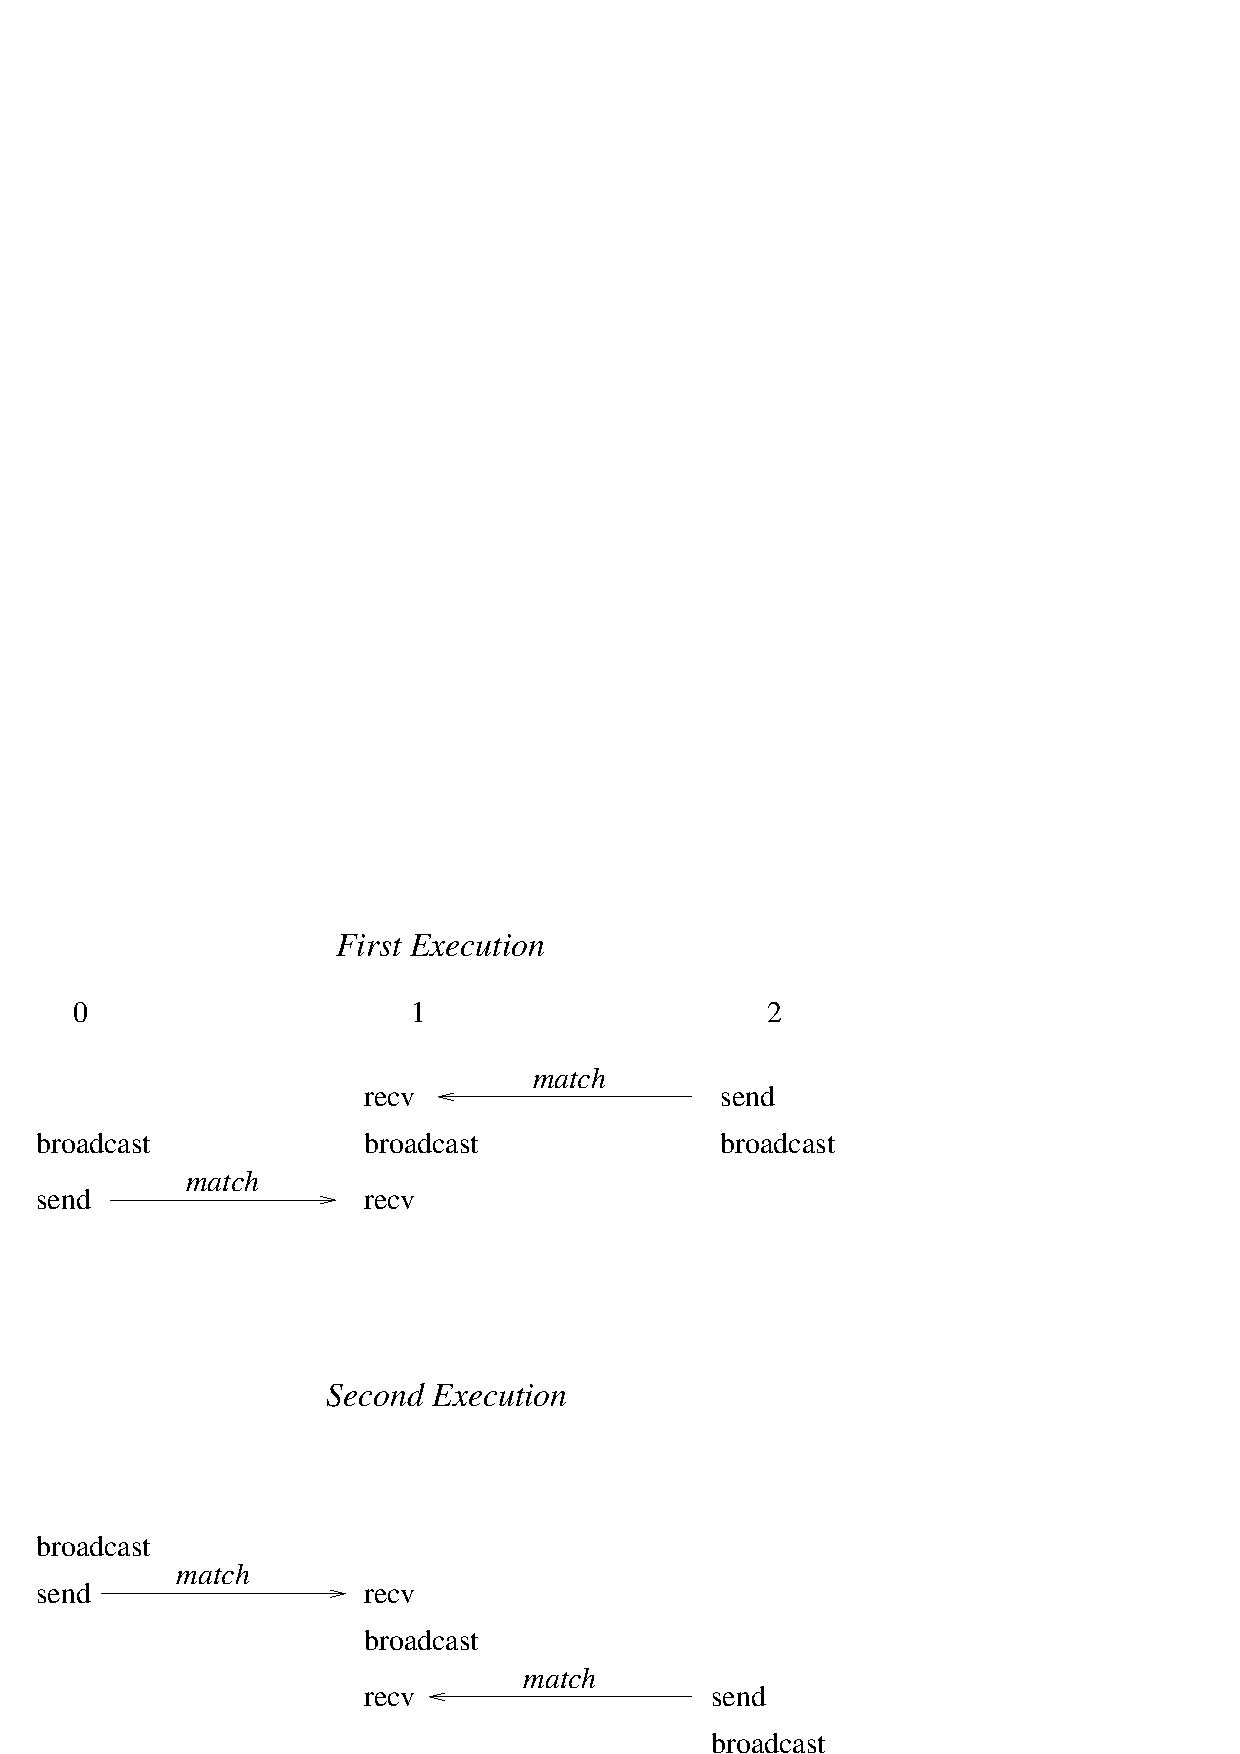
\includegraphics[width=4.00in]{figures/coll-matchings}}
  \caption[Race conditions with point-to-point and collective
    communications]{A race condition causes nondeterministic matching of sends
    and receives.  One cannot rely on synchronization from a broadcast
    to make the program deterministic.}
  \label{fig-coll-exN}
\end{figure}

Finally, in multithreaded implementations, one can have more than one,
concurrently executing, collective communication initialization call at an \MPI/ process.
In these situations, it is the user's responsibility to ensure that
the same communicator is not used concurrently by two different
collective communication initialization calls at the same \MPI/ process.
Collective communication initialization calls include
all calls for blocking collective operations,
all initiation calls for nonblocking collective operations, and
all initialization calls for persistent collective operations.

\begin{implementors}
Assume that broadcast is implemented using point-to-point \MPI/ communication.
Suppose the following two rules are followed.
\begin{enumerate}
\item
All receives specify their source explicitly (no wildcards).
\item
Each \MPI/ process sends all messages that pertain to one collective call before
sending any message that pertain to a subsequent collective call.
\end{enumerate}
Then, messages belonging to successive broadcasts cannot be confused,
as the order of point-to-point messages is preserved.

It is the implementor's responsibility to
ensure that point-to-point messages are not confused with collective
messages.  One way to accomplish this is, whenever a communicator is
created, to also create a ``hidden communicator''\mpitermindex{communicator!hidden} for collective communication.
One could achieve a similar
effect more cheaply, for example, by using a hidden
tag or context bit to indicate
whether the communicator is used for point-to-point or collective
communication.
\end{implementors}

\begin{example}
\label{coll-nbexN1}
\exindex{Mixing blocking and nonblocking collective operations}%
\Exindex{C}{Mixing blocking and nonblocking collective operations}{MPI\_Ibarrier,MPI\_Bcast,MPI\_Wait}%
Blocking and nonblocking collective operations can be interleaved, i.e.,
a blocking collective operation can be posted even if there is a
nonblocking collective operation outstanding.

%%HEADER
%%LANG: C
%%FRAGMENT
%%SKIPELIPSIS
%%DECL: int buf1[1], count; MPI_Datatype type; MPI_Comm comm;
%%ENDHEADER
\begin{lstlisting}[language={[MPI]C}]
MPI_Request req;

MPI_Ibarrier(comm, &req);
MPI_Bcast(buf1, count, type, 0, comm);
MPI_Wait(&req, MPI_STATUS_IGNORE);
\end{lstlisting}

Each \MPI/ process starts a nonblocking barrier operation, participates in a
blocking broadcast and then waits until every other \MPI/ process started the
barrier operation. This effectively turns the broadcast into a
synchronizing broadcast with possible communication/communication
overlap (\cfunc{MPI\_Bcast}\mpifuncindex{MPI\_BCAST} is allowed, but not required to
synchronize).
\end{example}


\begin{example}
\label{coll-nbexN2}
\exindex{False matching of collective operations}%
\Exindex{C}{Erroneous matching of collectives}{MPI\_Ibarrier,MPI\_Bcast,MPI\_Wait}%
The starting order of collective operations on a particular communicator
defines their matching. The following example shows an erroneous
matching of different collective operations on the same communicator.

%%HEADER
%%LANG: C
%%FRAGMENT
%%DECL: int rank, count, buf1[1]; MPI_Comm comm; MPI_Datatype type;
%%ENDHEADER
\begin{lstlisting}[language={[MPI]C}]
/* ---------------- THIS EXAMPLE IS ERRONEOUS --------------- */
MPI_Request req;
switch(rank) {
    case 0:
        /* erroneous matching */
        MPI_Ibarrier(comm, &req);
        MPI_Bcast(buf1, count, type, 0, comm);
        MPI_Wait(&req, MPI_STATUS_IGNORE);
        break;
    case 1:
        /* erroneous matching */
        MPI_Bcast(buf1, count, type, 0, comm);
        MPI_Ibarrier(comm, &req);
        MPI_Wait(&req, MPI_STATUS_IGNORE);
        break;
}
\end{lstlisting}

This ordering would match \cfunc{MPI\_Ibarrier}\mpifuncindex{MPI\_IBARRIER} on rank 0 with
\cfunc{MPI\_Bcast}\mpifuncindex{MPI\_BCAST} on rank 1, which is erroneous and the program behavior is
undefined. However, if such an order is required, the user must create
different duplicate communicators and perform the operations on them.
If started with two \MPI/ processes, the following program would be correct:

%%HEADER
%%LANG: C
%%FRAGMENT
%%DECL: int rank, buf1[1], count; MPI_Datatype type; MPI_Comm comm;
%%ENDHEADER
\begin{lstlisting}[language={[MPI]C}]
MPI_Request req;
MPI_Comm dupcomm;
MPI_Comm_dup(comm, &dupcomm);
switch(rank) {
    case 0:
        MPI_Ibarrier(comm, &req);
        MPI_Bcast(buf1, count, type, 0, dupcomm);
        MPI_Wait(&req, MPI_STATUS_IGNORE);
        break;
    case 1:
        MPI_Bcast(buf1, count, type, 0, dupcomm);
        MPI_Ibarrier(comm, &req);
        MPI_Wait(&req, MPI_STATUS_IGNORE);
        break;
}
\end{lstlisting}

\end{example}

\begin{users}
The use of different communicators offers some flexibility regarding the
matching of nonblocking collective operations. In this sense,
communicators could be used as an equivalent to tags. However,
communicator construction might induce overheads so that this should be
used carefully.
\end{users}


\begin{example}
\label{coll-nbexN3}
\exindex{Progress of nonblocking collective operations}%
\Exindex{C}{Progress of nonblocking collectives}{MPI\_Ibarrier,MPI\_Send,MPI\_Recv,MPI\_Wait}%
Nonblocking collective operations can rely on the similar progress rules
as nonblocking point-to-point operations. Thus, if started with two
\MPI/ processes, the following program is a valid \MPI/ program and is
guaranteed to terminate:

%%HEADER
%%LANG: C
%%FRAGMENT
%%SKIPELIPSIS
%%DECL: MPI_Comm comm; MPI_Datatype dtype;  int buf[1], count, tag, rank;
%%ENDHEADER
\begin{lstlisting}[language={[MPI]C}]
MPI_Request req;

switch(rank) {
    case 0:
      MPI_Ibarrier(comm, &req);
      MPI_Wait(&req, MPI_STATUS_IGNORE);
      MPI_Send(buf, count, dtype, 1, tag, comm);
      break;
    case 1:
      MPI_Ibarrier(comm, &req);
      MPI_Recv(buf, count, dtype, 0, tag, comm, MPI_STATUS_IGNORE);
      MPI_Wait(&req, MPI_STATUS_IGNORE);
      break;
}
\end{lstlisting}

The \MPI/ library must \mpitermni{progress}\mpitermindex{progress!nonblocking collective communication}\mpitermindex{collective communication!nonblocking!progress}\mpitermindex{semantics!collective communications!nonblocking progress}
the barrier in the \cfunc{MPI\_Recv}\mpifuncindex{MPI\_RECV}
call. Thus, the \cfunc{MPI\_Wait}\mpifuncindex{MPI\_WAIT} call in rank 0 will eventually
complete, which enables the matching \cfunc{MPI\_Send}\mpifuncindex{MPI\_SEND} so all calls
eventually return.

\end{example}

\begin{example}
\label{coll-nbexN4}
\exindex{Blocking/Nonblocking collectives do not match}
\Exindex{C}{Erroneous matching of blocking and nonblocking collectives}{MPI\_Ialltoall,MPI\_Alltoall,MPI\_Wait}%
Blocking and nonblocking collective operations do not match. The
following example is erroneous.

%%HEADER
%%LANG: C
%%FRAGMENT
%%DECL: int rank, scnt, rcnt; MPI_Comm comm; MPI_Datatype stype, rtype;
%%DECL: int sbuf[1], rbuf[1];
%%ENDHEADER
\begin{lstlisting}[language={[MPI]C}]
/* ---------------- THIS EXAMPLE IS ERRONEOUS --------------- */
MPI_Request req;

switch(rank) {
    case 0:
      /* erroneous false matching of Alltoall and Ialltoall */
      MPI_Ialltoall(sbuf, scnt, stype, rbuf, rcnt, rtype, comm, &req);
      MPI_Wait(&req, MPI_STATUS_IGNORE);
      break;
    case 1:
      /* erroneous false matching of Alltoall and Ialltoall */
      MPI_Alltoall(sbuf, scnt, stype, rbuf, rcnt, rtype, comm);
      break;
}
\end{lstlisting}
\end{example}



\begin{example}
\label{coll-nbexN5}
\exindex{Mixing collective and point-to-point requests}%
\Exindex{C}{Mixing collective and point-to-point}{MPI\_Ibarrier,MPI\_Send,MPI\_Irecv,MPI\_Waitall,MPI\_Wait}%
Collective and point-to-point requests can be mixed in functions that
enable multiple completions. If started with two \MPI/ processes, the
following program is valid.

%%HEADER
%%LANG: C
%%FRAGMENT
%%DECL: MPI_Comm comm; int buf[1], count, tag, rank; MPI_Datatype dtype;
%%ENDHEADER
\begin{lstlisting}[language={[MPI]C}]
MPI_Request reqs[2];

switch(rank) {
    case 0:
      MPI_Ibarrier(comm, &reqs[0]);
      MPI_Send(buf, count, dtype, 1, tag, comm);
      MPI_Wait(&reqs[0], MPI_STATUS_IGNORE);
      break;
    case 1:
      MPI_Irecv(buf, count, dtype, 0, tag, comm, &reqs[0]);
      MPI_Ibarrier(comm, &reqs[1]);
      MPI_Waitall(2, reqs, MPI_STATUSES_IGNORE);
      break;
}
\end{lstlisting}

The \cfunc{MPI\_Waitall}\mpifuncindex{MPI\_WAITALL} call returns only after the barrier and the receive completed.

\end{example}

\begin{example}
\label{coll-nbexN6}
\exindex{Pipelining nonblocking collective operations}%
\Exindex{C}{Pipelining nonblocking collectives}{MPI\_Ibcast,MPI\_Waitall}%
Multiple nonblocking collective operations can be outstanding on a
single communicator and match in order.

%%HEADER
%%LANG: C
%%FRAGMENT
%%DECL: int buf1[1], buf2[1], buf3[1], count; MPI_Datatype type; MPI_Comm comm;
%%DECL: void compute(int*);
%%ENDHEADER
\begin{lstlisting}[language={[MPI]C}]
MPI_Request reqs[3];

compute(buf1);
MPI_Ibcast(buf1, count, type, 0, comm, &reqs[0]);
compute(buf2);
MPI_Ibcast(buf2, count, type, 0, comm, &reqs[1]);
compute(buf3);
MPI_Ibcast(buf3, count, type, 0, comm, &reqs[2]);
MPI_Waitall(3, reqs, MPI_STATUSES_IGNORE);
\end{lstlisting}

\end{example}

\begin{users}
Pipelining and double-buffering techniques can efficiently be used to
overlap computation and communication. However, having too many
outstanding requests might have a negative impact on performance.
\end{users}

\begin{implementors}
The use of pipelining may generate many outstanding requests. A
high-quality hardware-supported implementation with limited resources
should be able to fall back to a software implementation if its
resources are exhausted. In this way, the implementation could limit the
number of outstanding requests only by the available memory.
\end{implementors}

\begin{example}
\label{coll-nbexN7}
\exindex{Overlapping communicators}%
\Exindex{C}{Overlapping communicators and collectives}{MPI\_Iallreduce,MPI\_Waitall}%
Nonblocking collective operations can also be used to enable
simultaneous collective operations on multiple overlapping
communicators (see Figure~\ref{overlap_comms}). The following example is started with three \MPI/ processes and
three communicators. The first communicator \code{comm1} includes ranks 0 and
1, \code{comm2} includes ranks 1 and 2, and \code{comm3} spans ranks 0 and 2. It is not
possible to perform a blocking collective operation on all communicators
because there exists no deadlock-free order to invoke them. However,
nonblocking collective operations can easily be used to achieve this
task.

%%HEADER
%%LANG: C
%%FRAGMENT
%%DECL: int rank, count; MPI_Comm comm1,comm2,comm3; MPI_Datatype dtype;
%%DECL: int sbuf1[1], rbuf1[1], sbuf2[1], rbuf2[1], sbuf3[1], rbuf3[1];
%%ENDHEADER
\begin{lstlisting}[language={[MPI]C},basicstyle=\lstsmall]
MPI_Request reqs[2];

switch(rank) {
    case 0:
      MPI_Iallreduce(sbuf1, rbuf1, count, dtype, MPI_SUM, comm1, &reqs[0]);
      MPI_Iallreduce(sbuf3, rbuf3, count, dtype, MPI_SUM, comm3, &reqs[1]);
      break;
    case 1:
      MPI_Iallreduce(sbuf1, rbuf1, count, dtype, MPI_SUM, comm1, &reqs[0]);
      MPI_Iallreduce(sbuf2, rbuf2, count, dtype, MPI_SUM, comm2, &reqs[1]);
      break;
    case 2:
      MPI_Iallreduce(sbuf2, rbuf2, count, dtype, MPI_SUM, comm2, &reqs[0]);
      MPI_Iallreduce(sbuf3, rbuf3, count, dtype, MPI_SUM, comm3, &reqs[1]);
      break;
}
MPI_Waitall(2, reqs, MPI_STATUSES_IGNORE);
\end{lstlisting}

\end{example}

\begin{figure}[hb]
  \centerline{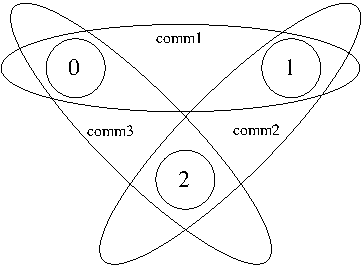
\includegraphics[width=2.50in]{figures/overlap_comms}}
  \caption[Overlapping communicators example]{Example with overlapping
  communicators}
  \label{overlap_comms}
\end{figure}

\begin{users}
This method can be useful if overlapping neighboring regions (halo
or ghost zones) are used in collective operations. The sequence of the
two calls in each \MPI/ process is irrelevant because the two nonblocking
operations are performed on different communicators.
\end{users}

\begin{example}
\label{coll-nbexN8}
\exindex{Independence of nonblocking operations}%
\Exindex{C}{Independence of nonblocking operations}{MPI\_Ibcast}%
The \mpitermni{progress}\mpitermindex{progress!nonblocking collective communication}\mpitermindex{collective communication!nonblocking!progress}\mpitermindex{semantics!collective communications!nonblocking progress}
of multiple outstanding nonblocking collective operations
is completely independent.

%%HEADER
%%LANG: C
%%FRAGMENT
%%DECL: int buf1[1], buf2[1], count; MPI_Comm comm; MPI_Datatype type;
%%DECL: void compute(int *);
%%ENDHEADER
\begin{lstlisting}[language={[MPI]C}]
MPI_Request reqs[2];

compute(buf1);
MPI_Ibcast(buf1, count, type, 0, comm, &reqs[0]);
compute(buf2);
MPI_Ibcast(buf2, count, type, 0, comm, &reqs[1]);
MPI_Wait(&reqs[1], MPI_STATUS_IGNORE);
/* nothing is known about the status of the first bcast here */
MPI_Wait(&reqs[0], MPI_STATUS_IGNORE);
\end{lstlisting}

Finishing the second \mpifunc{MPI\_IBCAST} is completely independent of
the first one. This means that it is not guaranteed that the first
broadcast operation is finished or even started after the second one is
completed via \code{reqs[1]}.
\end{example}

